\chapter{Mantle Convection Problem}\label{chap:evaluation}

Originally, the thermal evolution in mantle convection is modelled using the Stokes system of partial differential equations derived from the conservation equations of mass, momentum, and energy, in their simplest form of the Boussinesq approximation. Given an initial temperature, we can get a complete temperature time evolution predicted by the numerical solver, as shown below by the Figure \ref{figure:MC_workflow}:

\begin{figure}[H]
    \caption{Typical mantle convection workflow.}
    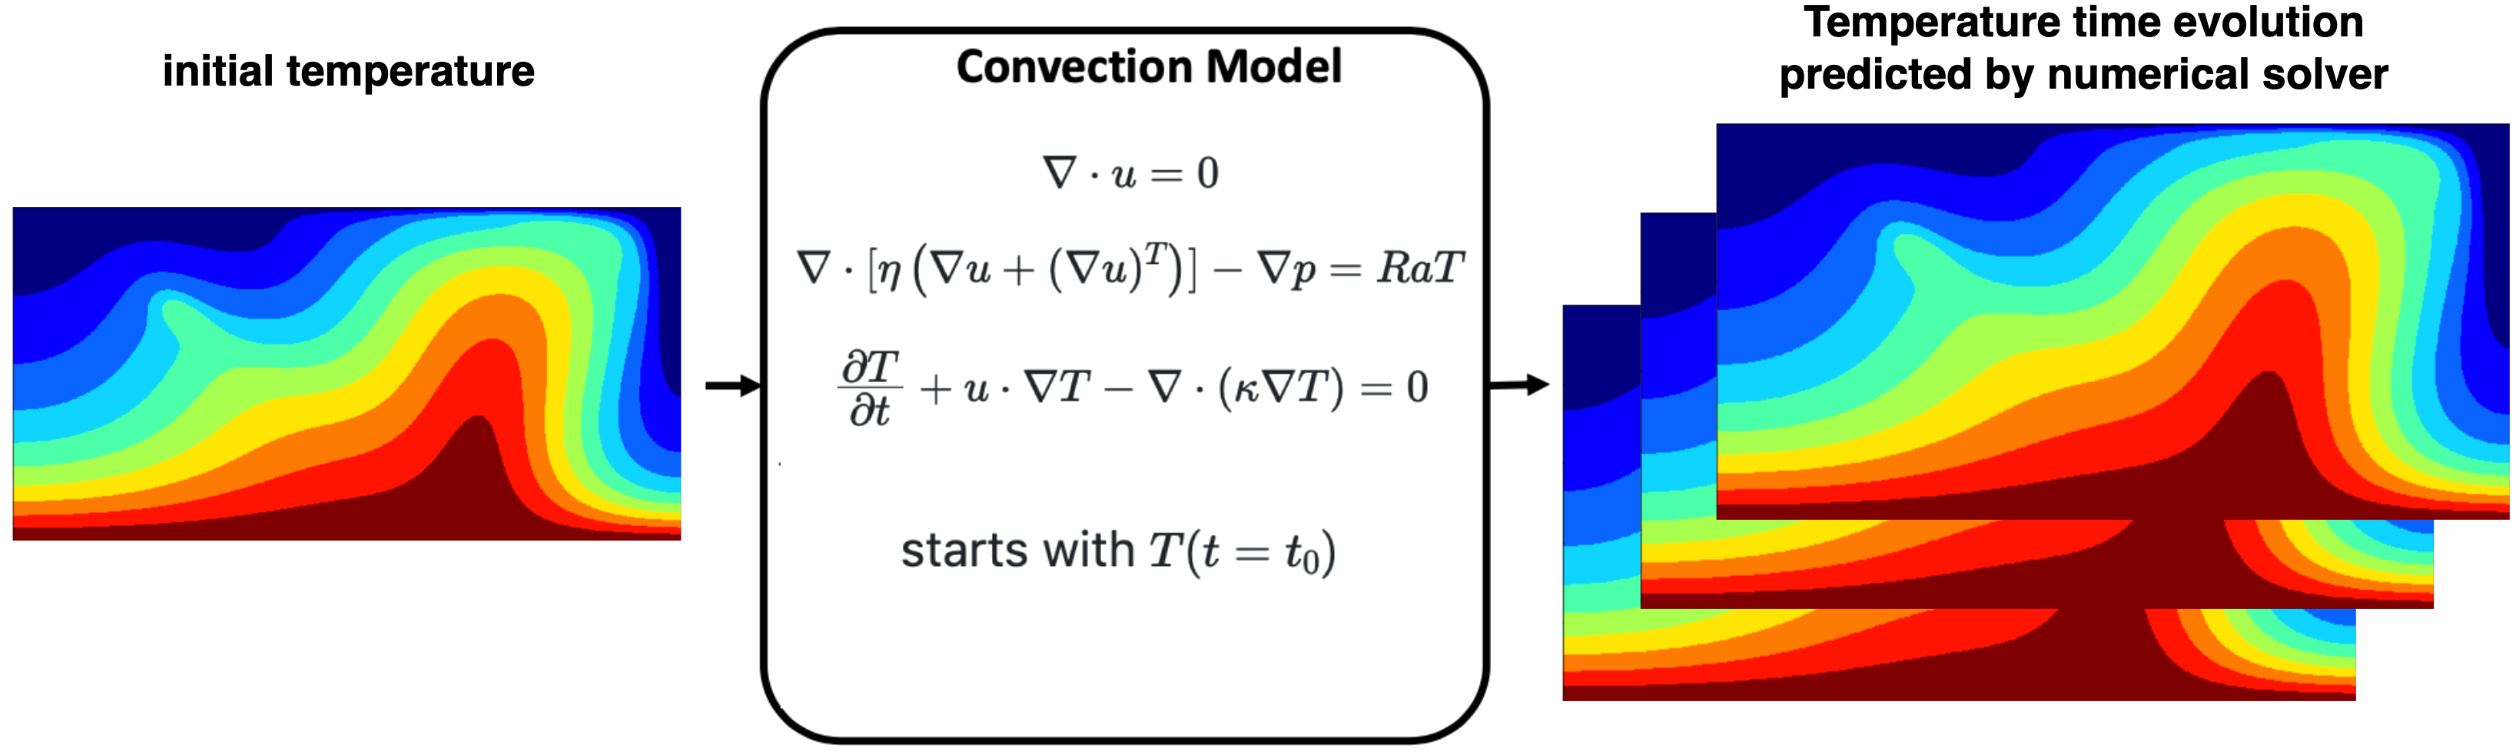
\includegraphics[scale=0.15]{figures/mantle_convection_images/Mantle_Convection_workflow.png}
    \label{figure:MC_workflow}
\end{figure}

To explore the usage of Neural Networks as surrogate models for the original mantle convection numerical solver to significantly reduce the computational
cost, three different datasets are tested, including Limited Dataset, Larger Dataset and Interpolated Dataset. Each dataset is composed of several temperature time-series with 100 timestamps each resulting from numerical simulations with randomly sampled initial conditions (except for the Interpolated Dataset, which is created from the Larger Dataset using interpolation).

\section{Mantle Convection Simulation on Limited Dataset}

The limited dataset consists of 100 files and each of them represents one mantle convection simulation in 100 time steps generated with an initial condition with random number of points and random amplitude and coordinates of Gaussian anomalies distributed in space (a total of 10000 temperature fields). Starting from each initial condition we convect as long as there is meaningful change in the simulation (that is the temperature fields change enough after one time-step). There are 100 temperature fields with a size of $201 \times 401$ for each of the 100 timestamps in a file and the time step has to be adaptive, otherwise the whole random generation of the initial condition would be hard to implement. This adaptive timestamps lead to a problem, that is, the distance between each consecutive pairs of time steps are not the same even in the same simulation file. This could lead to some uncommon behaviors when predicting a sequence of temperature fields using the ML architecture, which will be discussed in more details in the following sections.

Figure \ref{figure:temperature_field_sample} shows one random temperature fields in the dataset with the y-axis inverted and colored using 10-color-map (all the figures in this chapter will have their y-axis inverted and colored using 10-color-map as well, but without labels on x-axis and y-axis for better visualisation):

\begin{figure}[H]
    \caption{Temperature Field example. (For the colorbar of the upcoming figures, see this one.)}
    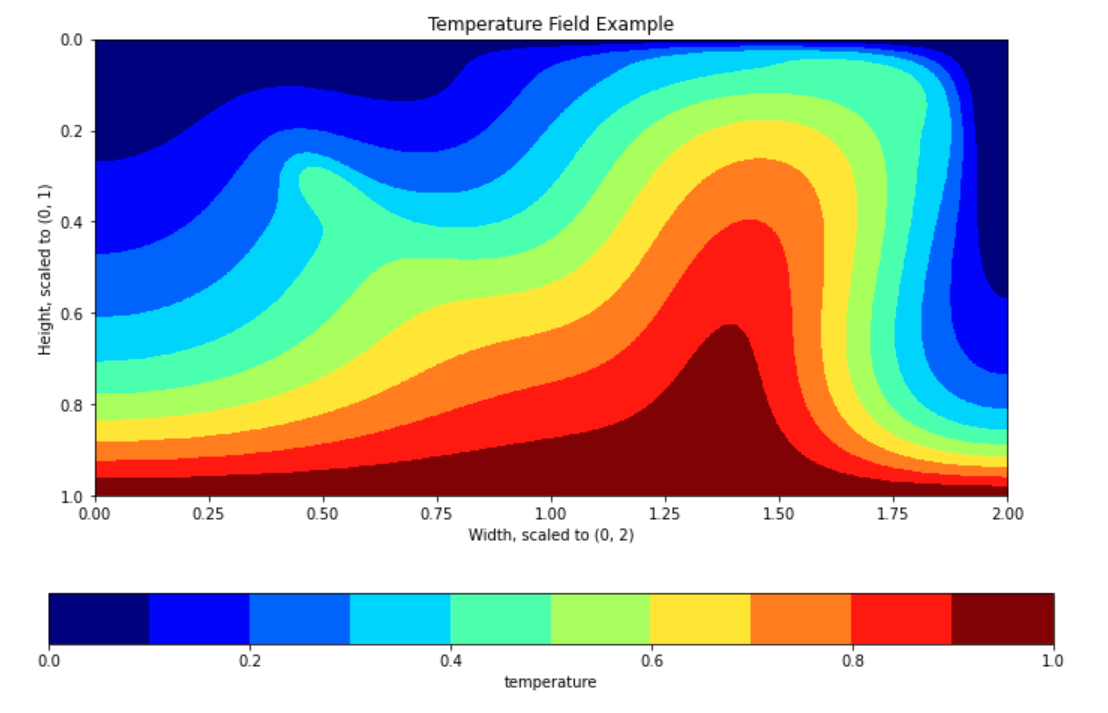
\includegraphics[scale=0.6]{figures/mantle_convection_images/temperature_field_example.png}
    \label{figure:temperature_field_sample}
\end{figure}

The entire dataset is randomly divided in a ratio of 8:1:1, where 80 per cent of the dataset is used for training, 10 per cent of the data for testing and the remaining 10 per cent to perform validation and prevent overfitting. However, the way we divide them is different in implementing the ConvAE, FNN and LSTM and will be discussed in more details in the following sections.

The dataset is uploaded to Gadi, a HPC system, for storage to make the training process more efficient. 

\subsection{Compression of temperature fields}

Since applying Machine Learning (ML) algorithms directly on the original sized temperature fields can take significantly more time to train the model and could possibly lead to the risk of over-parameterization, we decided to compress the temperature fields first before feeding the data into different ML architectures.

In this study, the overall process to solve the mantle convection problem would be: 

\begin{enumerate}
  \item Train the ConvAE.
  \item Train the FNN/LSTM using the latent space representation of both input and output data. (encoder from ConvAE is used to get the the latent space representation.)
  \item Test the predicted temperature in its original size. (decoder from ConvAE is used to get the original sized temperature from the latent space representation.)
\end{enumerate}

Figure \ref{figure:ConvAE_workflow}, Figure \ref{figure:FNN_workflow} and Figure \ref{figure:LSTM_workflow} below show the workflow ConvAE, FNN and LSTM respectively:

\begin{figure}[H]
    \centering
    \caption{Workflow of ConvAE.}
    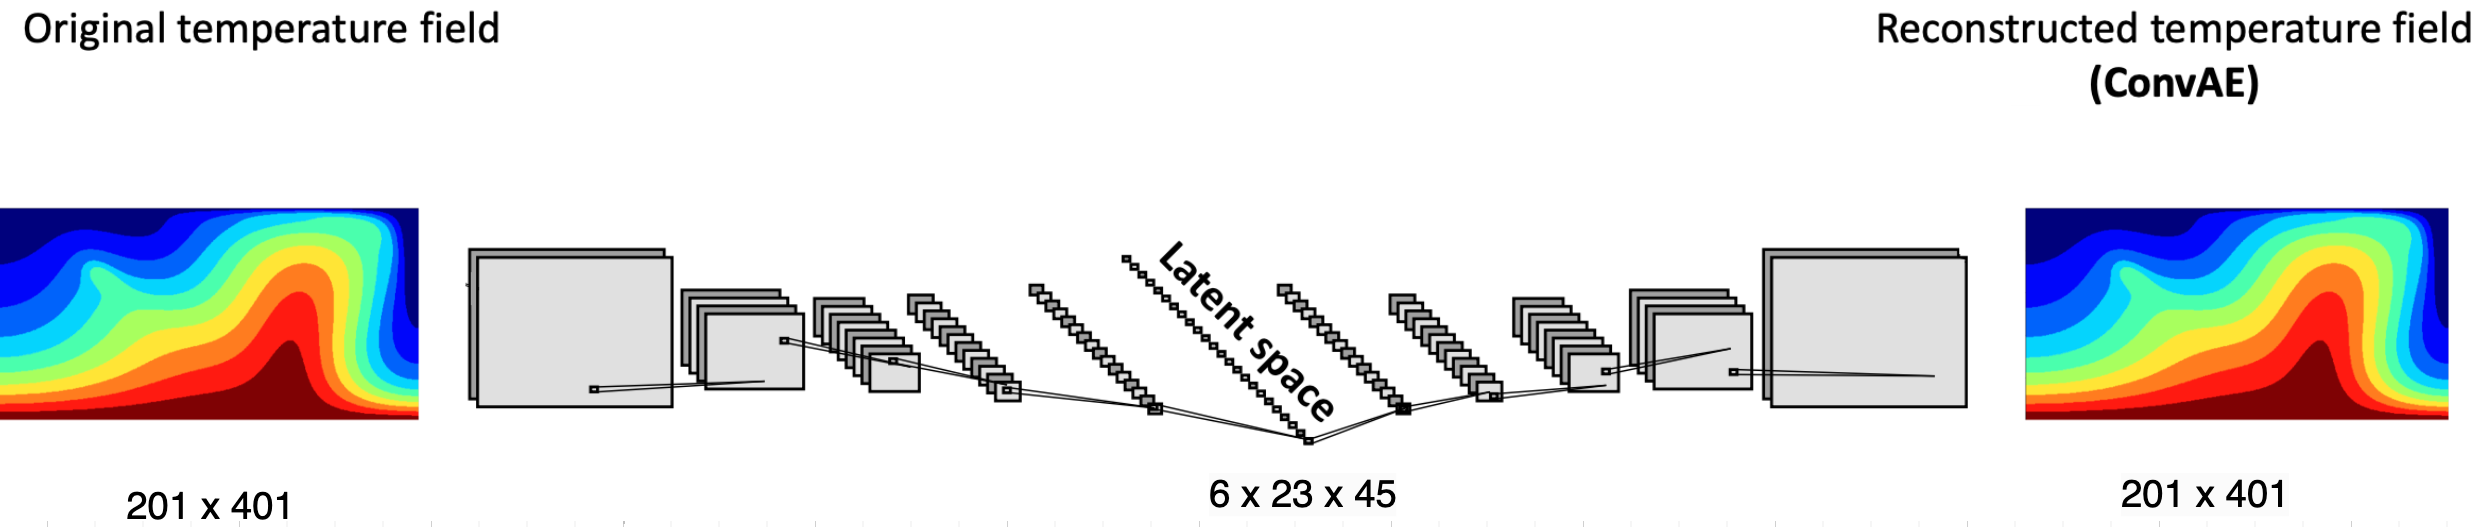
\includegraphics[scale=0.3]{figures/mantle_convection_images/ConvAE_workflow.png}
    \label{figure:ConvAE_workflow}
\end{figure}

\begin{figure}[H]
    \centering
    \caption{Workflow of FNN.}
    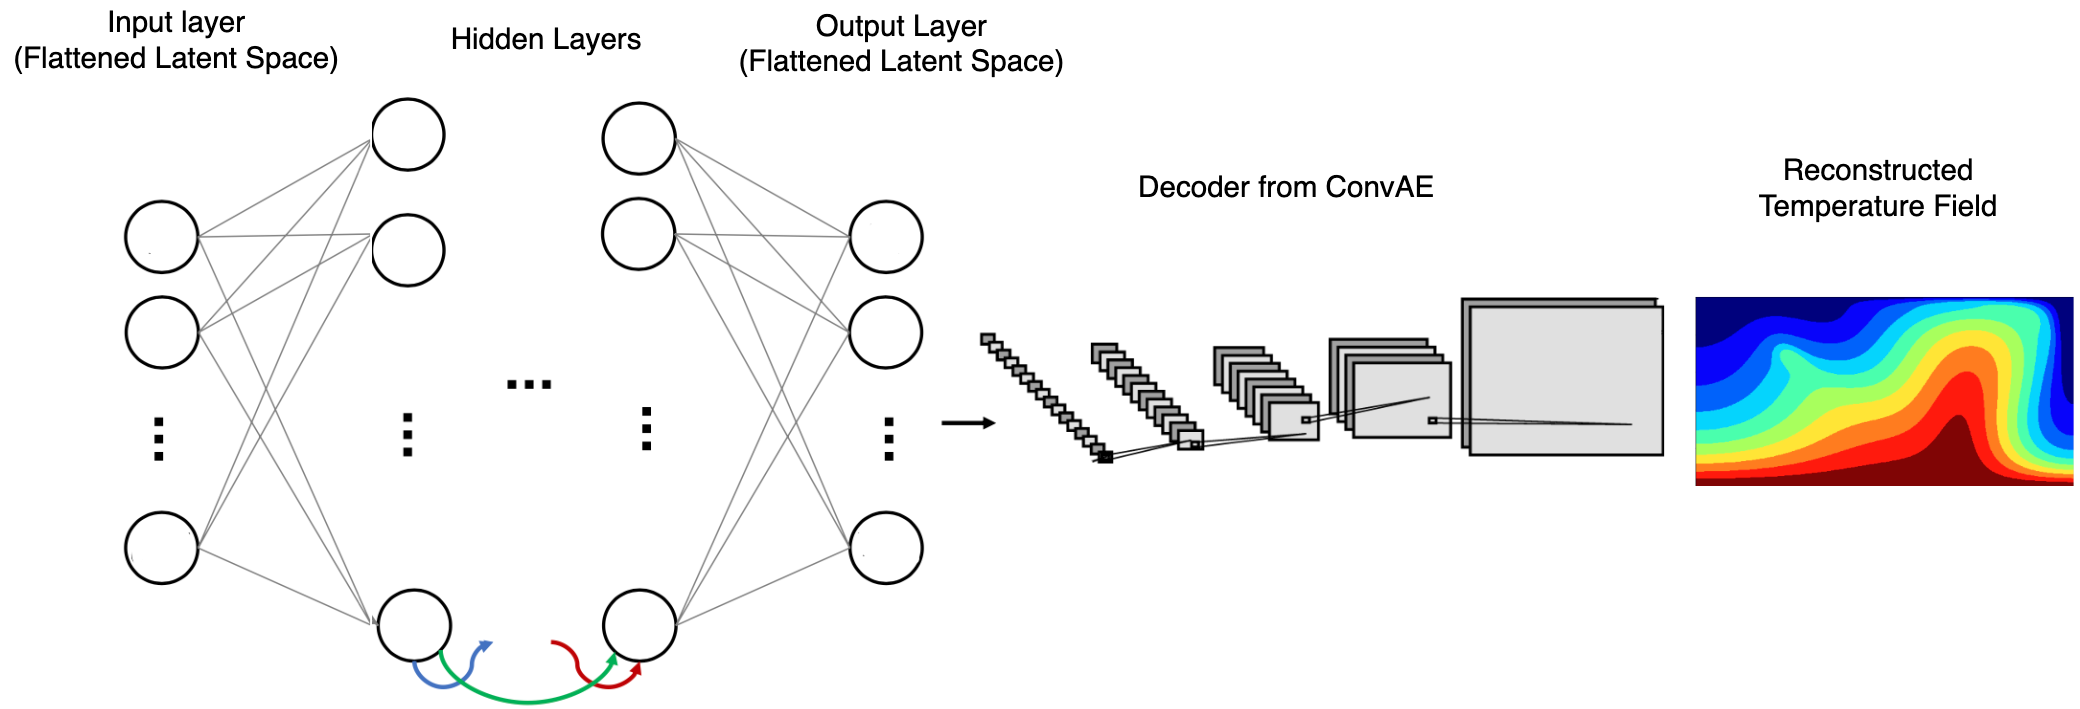
\includegraphics[scale=0.35]{figures/mantle_convection_images/FNN_workflow.png}
    \label{figure:FNN_workflow}
\end{figure}

\begin{figure}[H]
    \centering
    \caption{Simple Workflow of LSTM, where Tn is a temperature field in its latent space representation. Here we input the first 50 temperature fields (after compressed and flattened) from a simulation into the LSTM and hopefully LSTM would predict the rest 50 temperature fields of the same simulation (also compressed and flattened).(Source of the left figure: StackOverflow.)}
    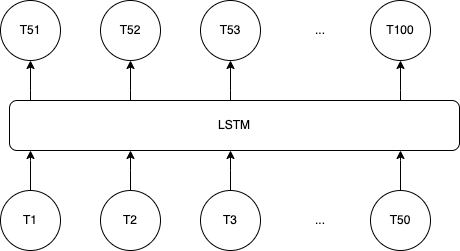
\includegraphics[scale=0.6]{figures/mantle_convection_images/LSTM_workflow.png}
    \label{figure:LSTM_workflow}
\end{figure}

The complete 10000 temperature fields are randomly shuffled and divided in a ratio of 80\%, 10\%, 10\% for training, testing and validation where each piece of data consists only one temperature field (fed as both the input and output during training and testing). Given the size of the training set, ConvAE is fed with a batch size of 16 temperature fields during the training to perform Mini-Batch Gradient Descent.

We find that ConvAE with a latent space size of $6 \times 23 \times 45$ offers an excellent compression factor of 13, while being able to reconstruct the temperature fields in its original size with the lowest data loss on the test set.

The architecture of the ConvAE in this case consists of two convolutional layers for the encoder and two transpose convolutional layers for the decoder. Both of these four layers have the size of the filter as $5 \times 5$ and a stride of $3 \times 3$. Tanh() is used as the activation function to introduce non-linearity between each layers (except for the last layer in the decoder) and mean square error (MSE) is used as the loss function. The model is trained for 1000 epochs on Gadi.

In the following figures, we present some detailed test results from this ConvAE, including the training loss and validation loss from Figure \ref{figure:ConvAE_limited_losses}, overall testing result from Figure \ref{figure:ConvAE_limited_testing}, and the most/least accurate prediction in Figure \ref{figure:ConvAE_limited_best_worst}:

\begin{figure}[H]
    \caption{Training loss and Validation loss of ConvAE trained with Limited Dataset.}
    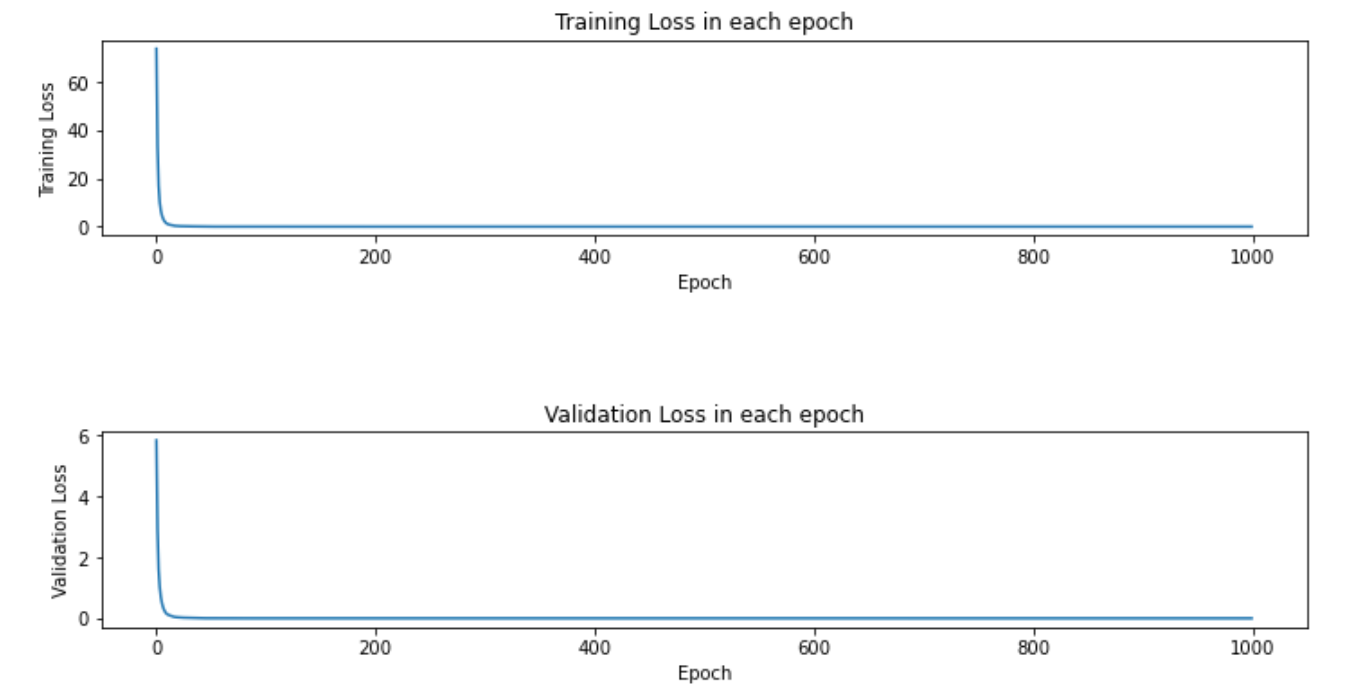
\includegraphics[scale=0.6]{figures/mantle_convection_images/limited_dataset/ConvAE_trainingData.png}
    \label{figure:ConvAE_limited_losses}
\end{figure}

\begin{figure}[H]
    \caption{Overall testing result of ConvAE trained with Limited Dataset.}
    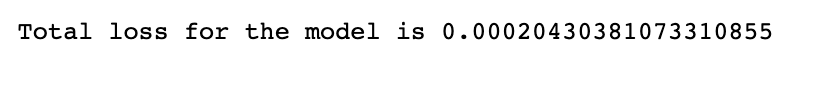
\includegraphics[scale=0.8]{figures/mantle_convection_images/limited_dataset/ConvAE_OverallTesting.png}
    \label{figure:ConvAE_limited_testing}
\end{figure}

\begin{figure}[H]
\centering
\begin{subfigure}{0.45\textwidth}
    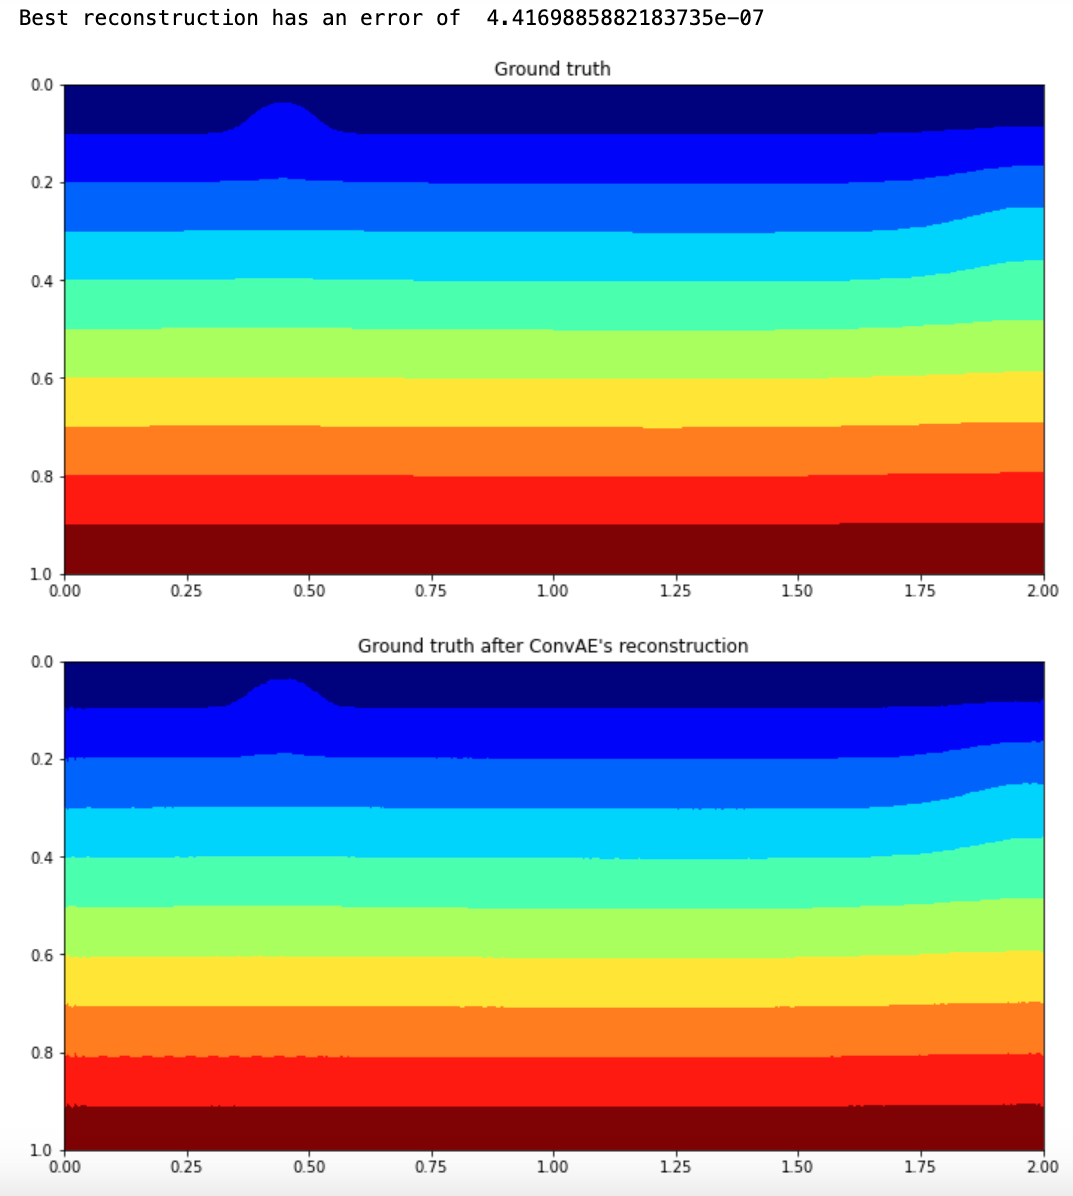
\includegraphics[width=\textwidth]{figures/mantle_convection_images/limited_dataset/ConvAE_Best.png}
    \caption{Most accurate reconstruction of ConvAE trained with Limited Dataset.}
\end{subfigure}
\hfill
\begin{subfigure}{0.45\textwidth}
    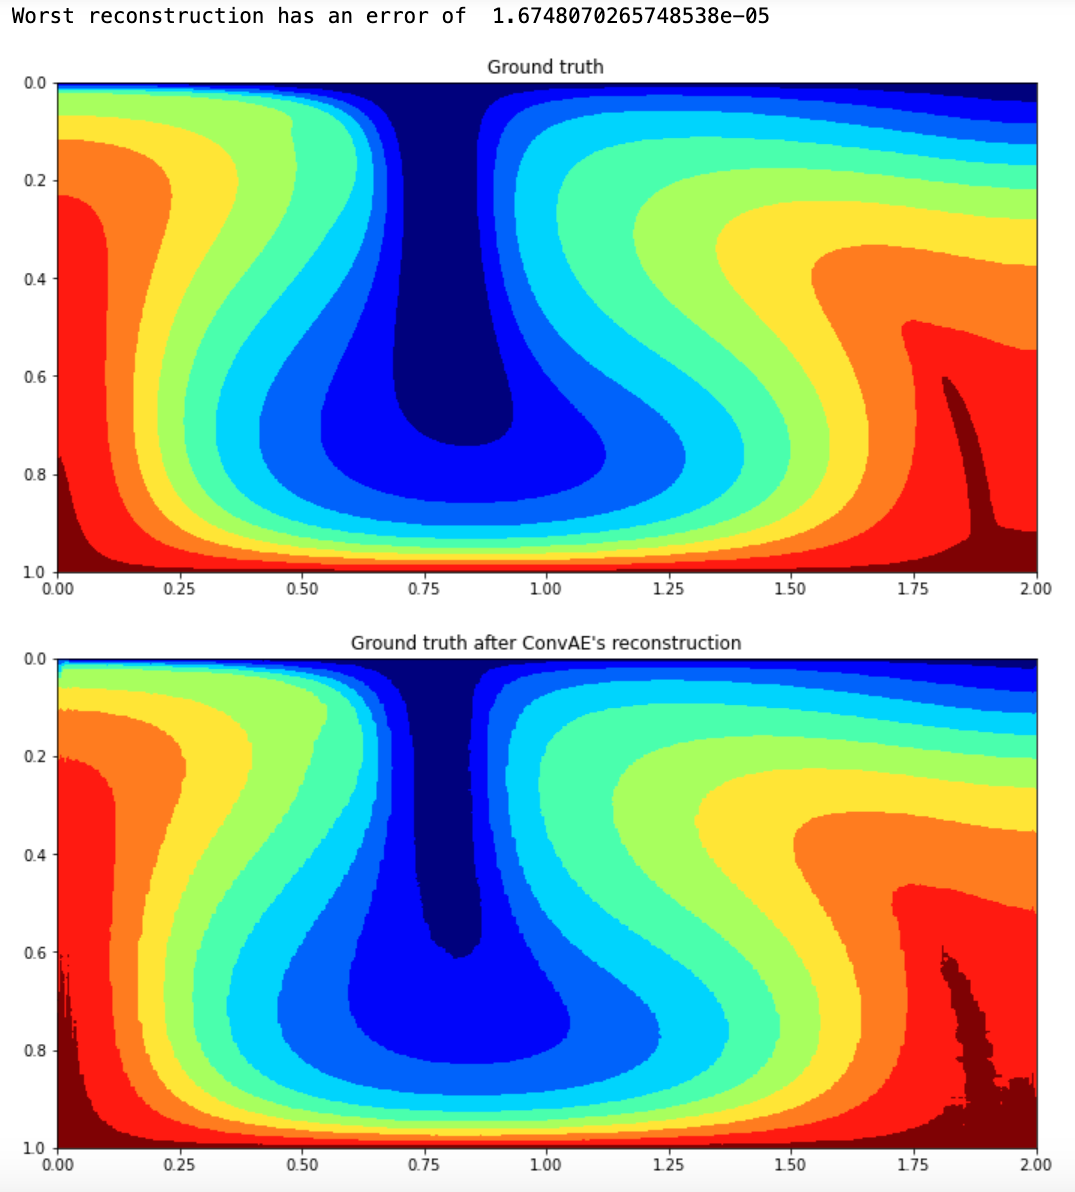
\includegraphics[width=\textwidth]{figures/mantle_convection_images/limited_dataset/ConvAE_Worst.png}
    \caption{Least accurate reconstruction of ConvAE trained with Limited Dataset.}
\end{subfigure}     
\caption{Best case and worst case using ConvAE.}
\label{figure:ConvAE_limited_best_worst}
\end{figure}


On average, the reconstruction loss are low and no overfitting occurs. However, we can observe that the ConvAE does not reconstructe the thin feature in the bottom right corner of the worst case. This could imply that the ConvAE works best for "smooth" input hence others with small scale length features will generally perform worse.

We also applied some POD (Proper Orthogonal Decomposition) analysis to the compressed-decompressed fields with contrast to the original temperature fields and the result is great as well, the figure to this analysis will be presented in the following sections as contrast to the POD analysis of the prediction model (FNN or LSTM) 


\subsection{Fully Connected Neural Network for Prediction}

We now move on to predict the latent space representation and our first candidate is the feedforward fully connected neural network (FNN). The FNN in this study uses each adjacent pair of temperature fields (e.g. $i$th and ($i+1$)th fields) as one training set, takes one temperature fields as the input and output the temperature fields at the next time step. Therefore, the dataset is reconstructed into 9900 pairs of temperature fields with consecutive timestamps. These pairs are randomly shuffled and divided in a ratio of 80\%, 10\%, 10\% for training, testing and validation where each piece of data consists two temperature field having consecutive timestamps.

Before the latent space representation is fed as the input of FNN, it is flattened into one dimension. The prediction result of FNN in this case is then resized from a one dimensional vector ($1 \times 6210$) to the shape of the latent space ($6 \times 23 \times 45$) before we applied further testing.

The learnable parameters of FNN are optimized using small mini-batches of 16 pairs of consecutive temperature fields and Adam as the optimizer, where the loss function is defined as the mean square error (MSE) between the prediction of FNN and the actual output (both in the shape of latent space representation, which is $6 \times 23 \times 45$).

After testing with FNNs that have different number of hidden layers and neurons per hidden layer, we found that architectures with a total number 3 hidden layers seemed to perform the best. (We also test some deeper architectures with 4-5 hidden layers. However, there is no significant reduction in the loss value)

In the following figures, we present results from a FNN with 3 hidden layers with 3105, 1035 and 3105 neurons, Tanh() as activation function, and trained for 1000 epochs. The figures include the training loss and validation loss from Figure \ref{figure:FNN_limited_losses}, overall testing result from Figure \ref{figure:FNN_limited_testing}, and the most/least accurate prediction in Figure \ref{figure:FNN_limited_best} and Figure \ref{figure:FNN_limited_worst}:

\begin{figure}[H]
    \caption{Training loss and Validation loss of FNN trained with Limited Dataset.}
    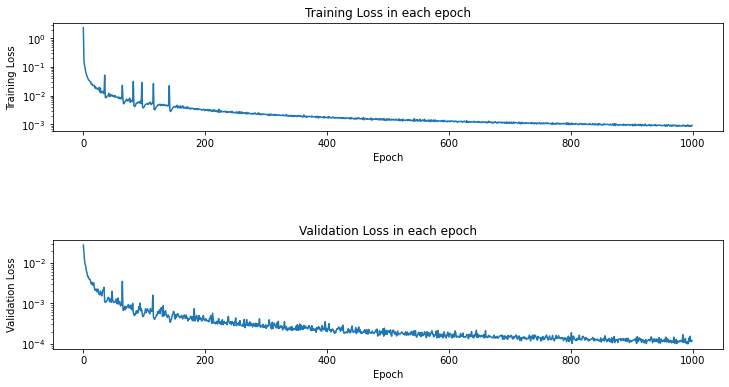
\includegraphics[scale=0.6]{figures/mantle_convection_images/limited_dataset/FNN_trainingData.png}
    \label{figure:FNN_limited_losses}
\end{figure}

\begin{figure}[H]
    \caption{Overall testing result of FNN trained with Limited Dataset.}
    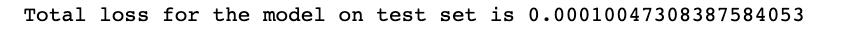
\includegraphics[scale=0.8]{figures/mantle_convection_images/limited_dataset/FNN_OverallTesting.png}
    \label{figure:FNN_limited_testing}
\end{figure}

\begin{figure}[H]
    \caption{Ground truth, ground truth after ConvAE's compression-decompression, and most accurate prediction of FNN trained with Limited Dataset.}
    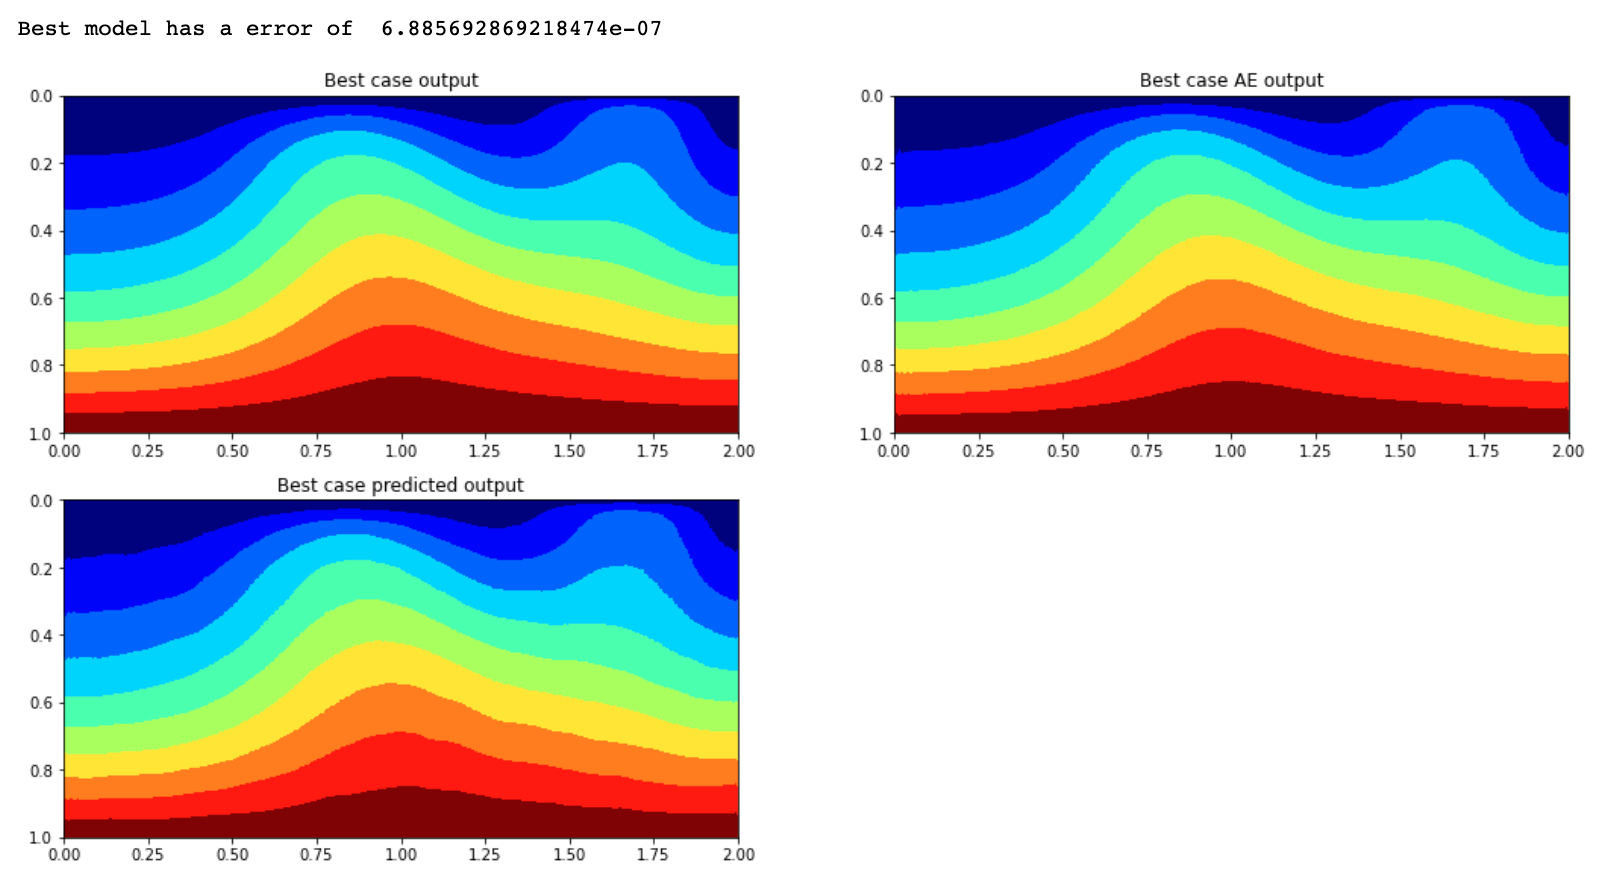
\includegraphics[scale=0.5]{figures/mantle_convection_images/limited_dataset/FNN_Best.png}
    \label{figure:FNN_limited_best}
\end{figure}

\begin{figure}[H]
    \caption{Ground truth, ground truth after ConvAE's compression-decompression, and least accurate prediction of FNN trained with Limited Dataset.}
    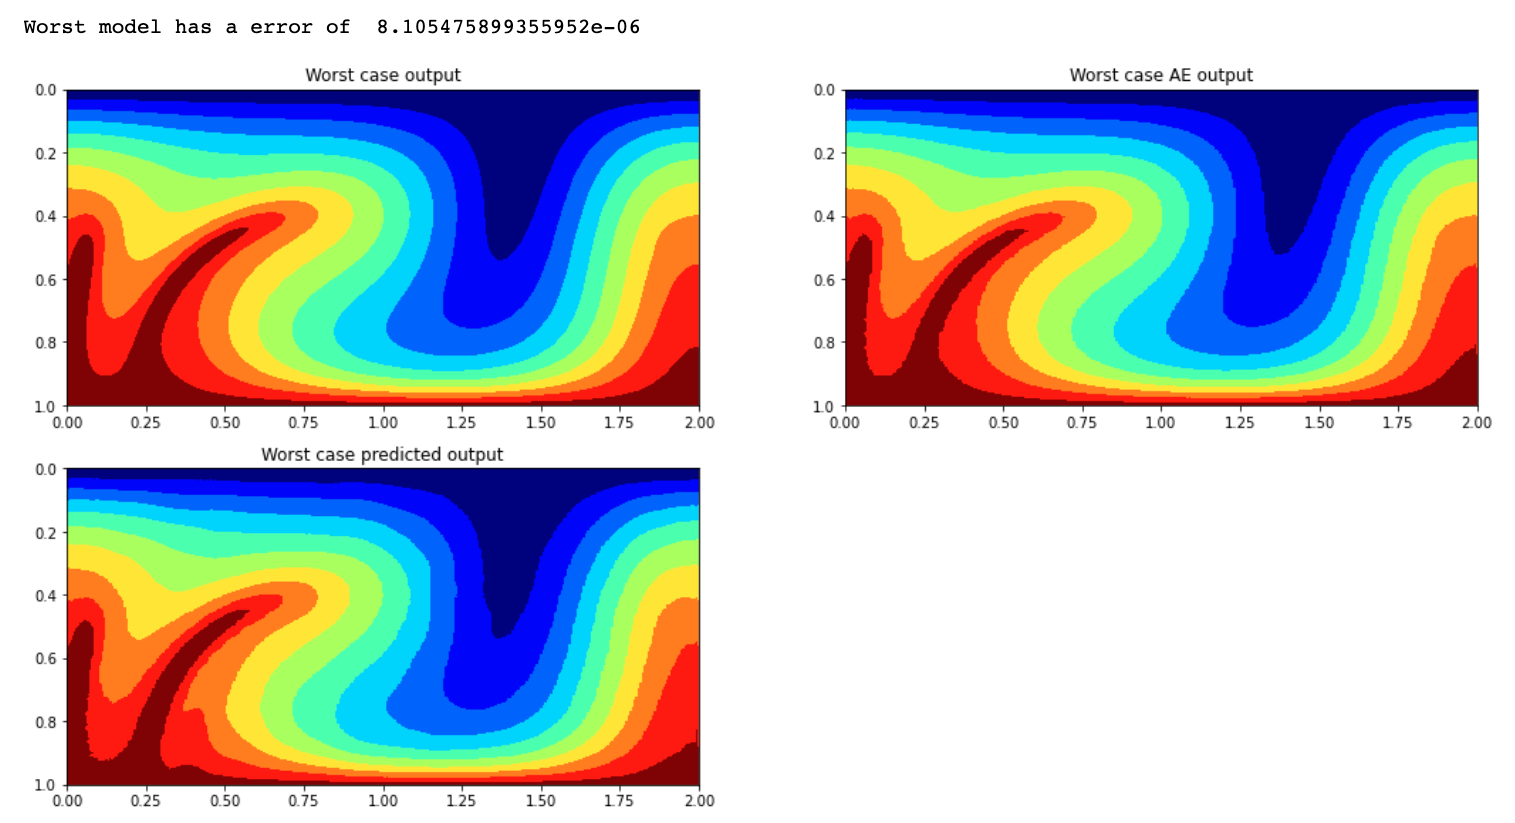
\includegraphics[scale=0.5]{figures/mantle_convection_images/limited_dataset/FNN_Worst.png}
    \label{figure:FNN_limited_worst}
\end{figure}

On average, the loss values are low and no overfitting occurs. The prediction for the temperature field at the next timestamp is able to capture the main features precisely with some small information loss, which is partially due to information loss caused by the compression-decompression process of ConvAE.

To further evaluate the performance of FNN in predicting a complete time series, two methods are tested on all 100 simulations one by one: 

\begin{enumerate}
  \item "One-for-All" (also referred as "Output-as-input Prediction"): Only take the first temperature field in the file as the input and use a prediction-as-input loop to get the rest of the 99 temperature fields. (use $T1$ from dataset $\rightarrow$ get predicted $T2$ $\rightarrow$ use predicted $T2$ $\rightarrow$ get predicted $T3$ $\rightarrow$ ...)
  \item "One-for-One" (also referred as "Single Prediction"): Constantly feed a temperature field from the original dataset and get the temperature field at the next time step as usual. (use $T1$ from dataset $\rightarrow$ get predicted $T2$ $\rightarrow$ use $T2$ from dataset $\rightarrow$ get predicted $T3$ $\rightarrow$ ...)
\end{enumerate}

In this case, the first method can reduce the computation complexity of the mantle convection problem more effectively than the second method, since we only need one initial input data and the model can generate the rest of the temperature field sequence. Therefore, the following best case and worst case will be evaluated using the data loss of the first method.

To better visualize the prediction result of the above two methods, two animations representing the best case and the worst case (evaluated based on the sum of MSE for each prediction using the first method) in the format of GIF files are generated. From top to bottom, the first picture represents the actual output from the dataset, the second one represents the prediction result using the first method, and the last one represents the prediction result using the second method.

Figure \ref{figure:FNN_limited_best_gif} and Figure \ref{figure:FNN_limited_worst_gif} show 10\% of the two sprite sheets converted from the original GIFs (every 10th frame) for the convenience of reading:

\begin{figure}[H]
    \centering
    \caption{Best case animation sheet of FNN trained with Limited Dataset (Link to this GIF: \url{https://drive.google.com/file/d/1Hmb4UlevBHMRw0jDScTwUzDFPbYNubKO/view?usp=sharing})}
    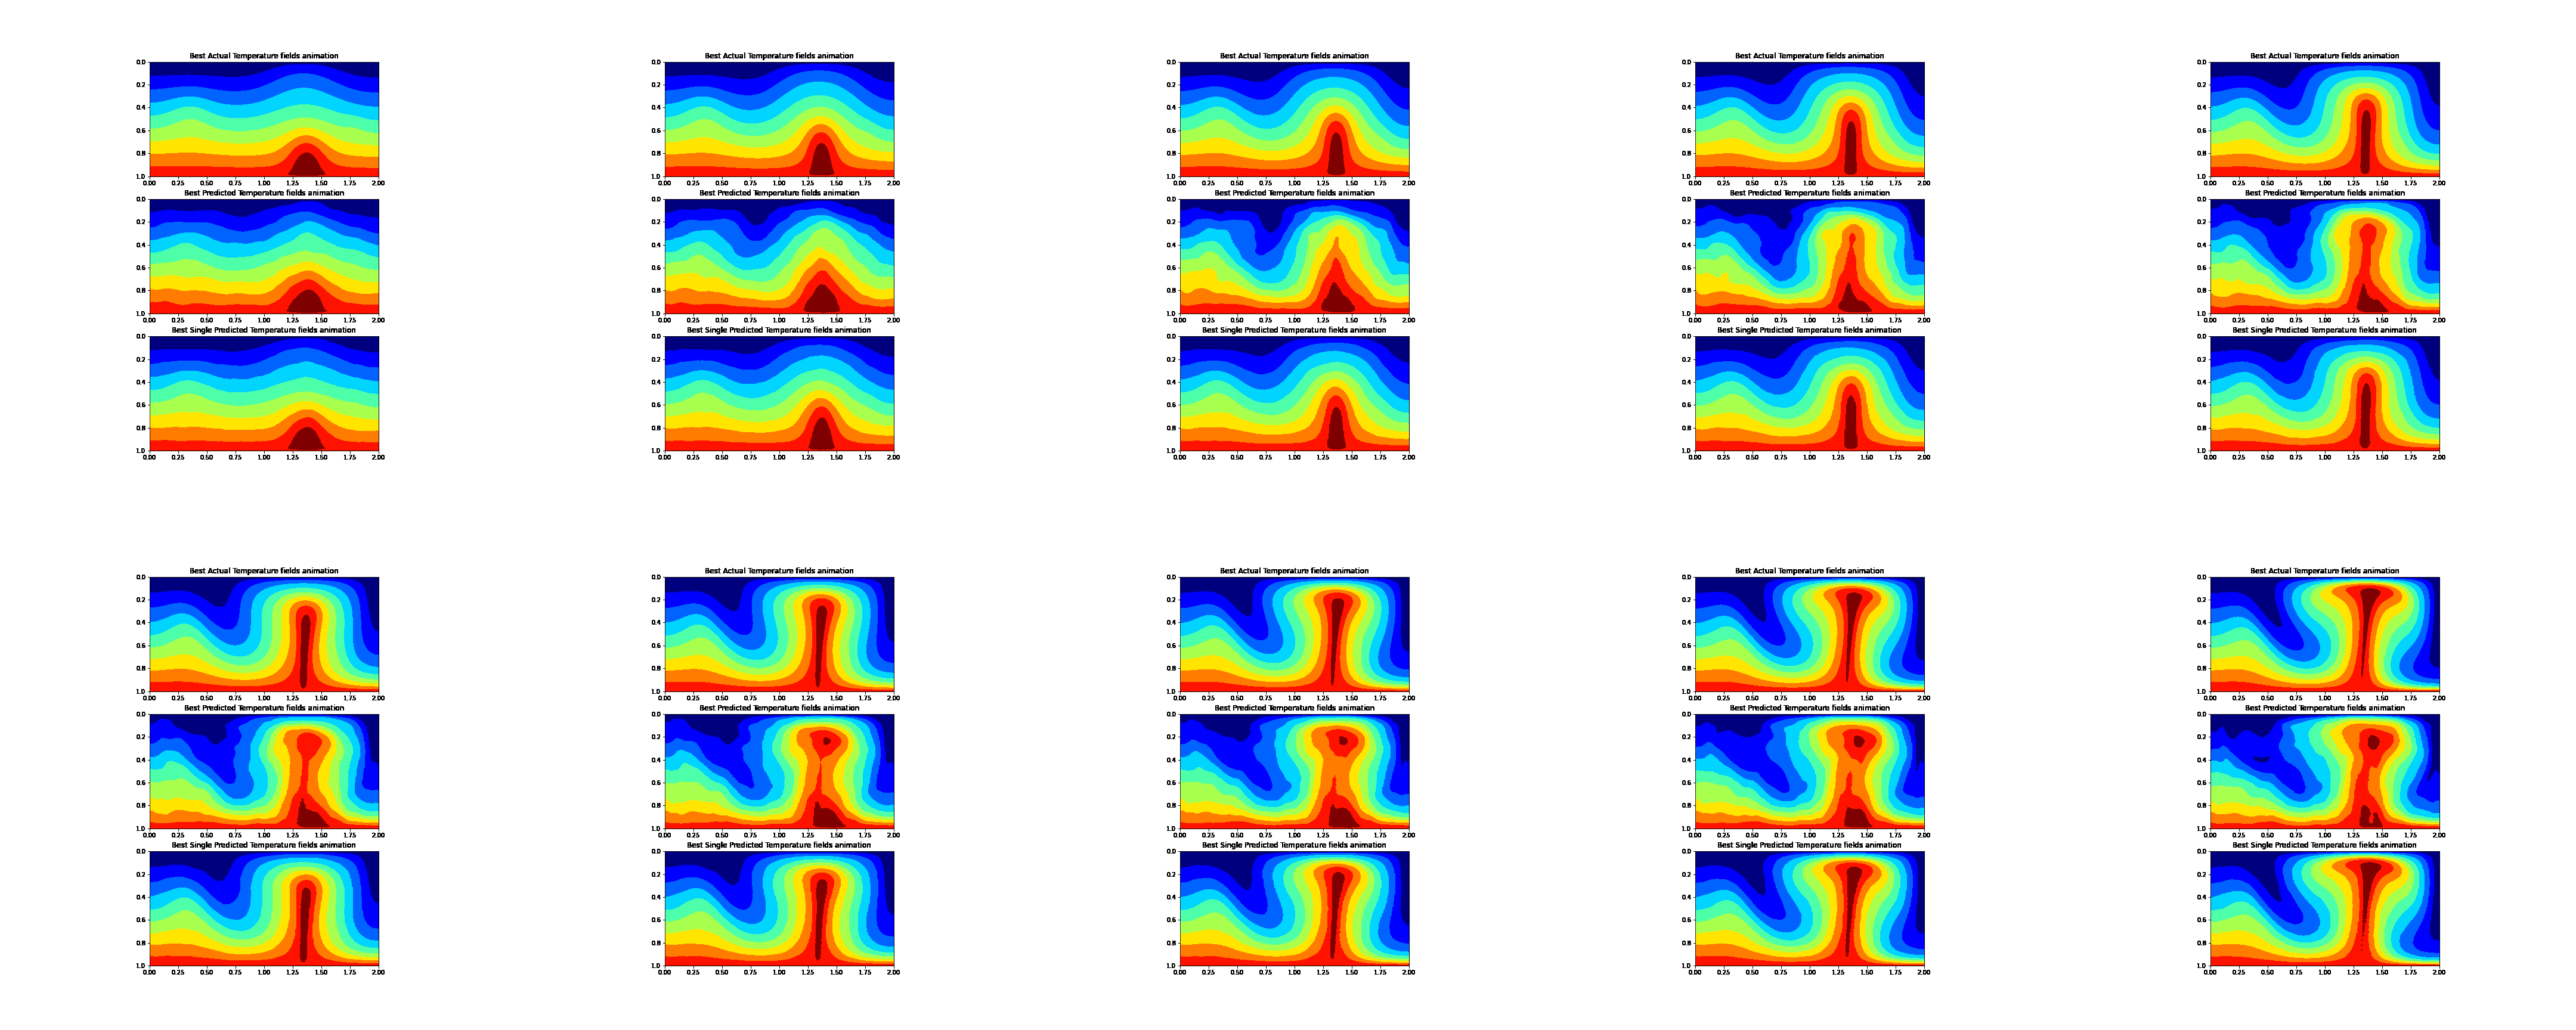
\includegraphics[scale=0.10]{figures/mantle_convection_images/limited_dataset/FNN_Best_GIF_sheet.png}
    \label{figure:FNN_limited_best_gif}
\end{figure}

\begin{figure}[H]
    \centering
    \caption{Worst case animation sheet of FNN trained with Limited Dataset (Link to this GIF: 
    \url{https://drive.google.com/file/d/11jRFxq-XuIUvTk74OuxswDn3u031k_q7/view?usp=sharing})}
    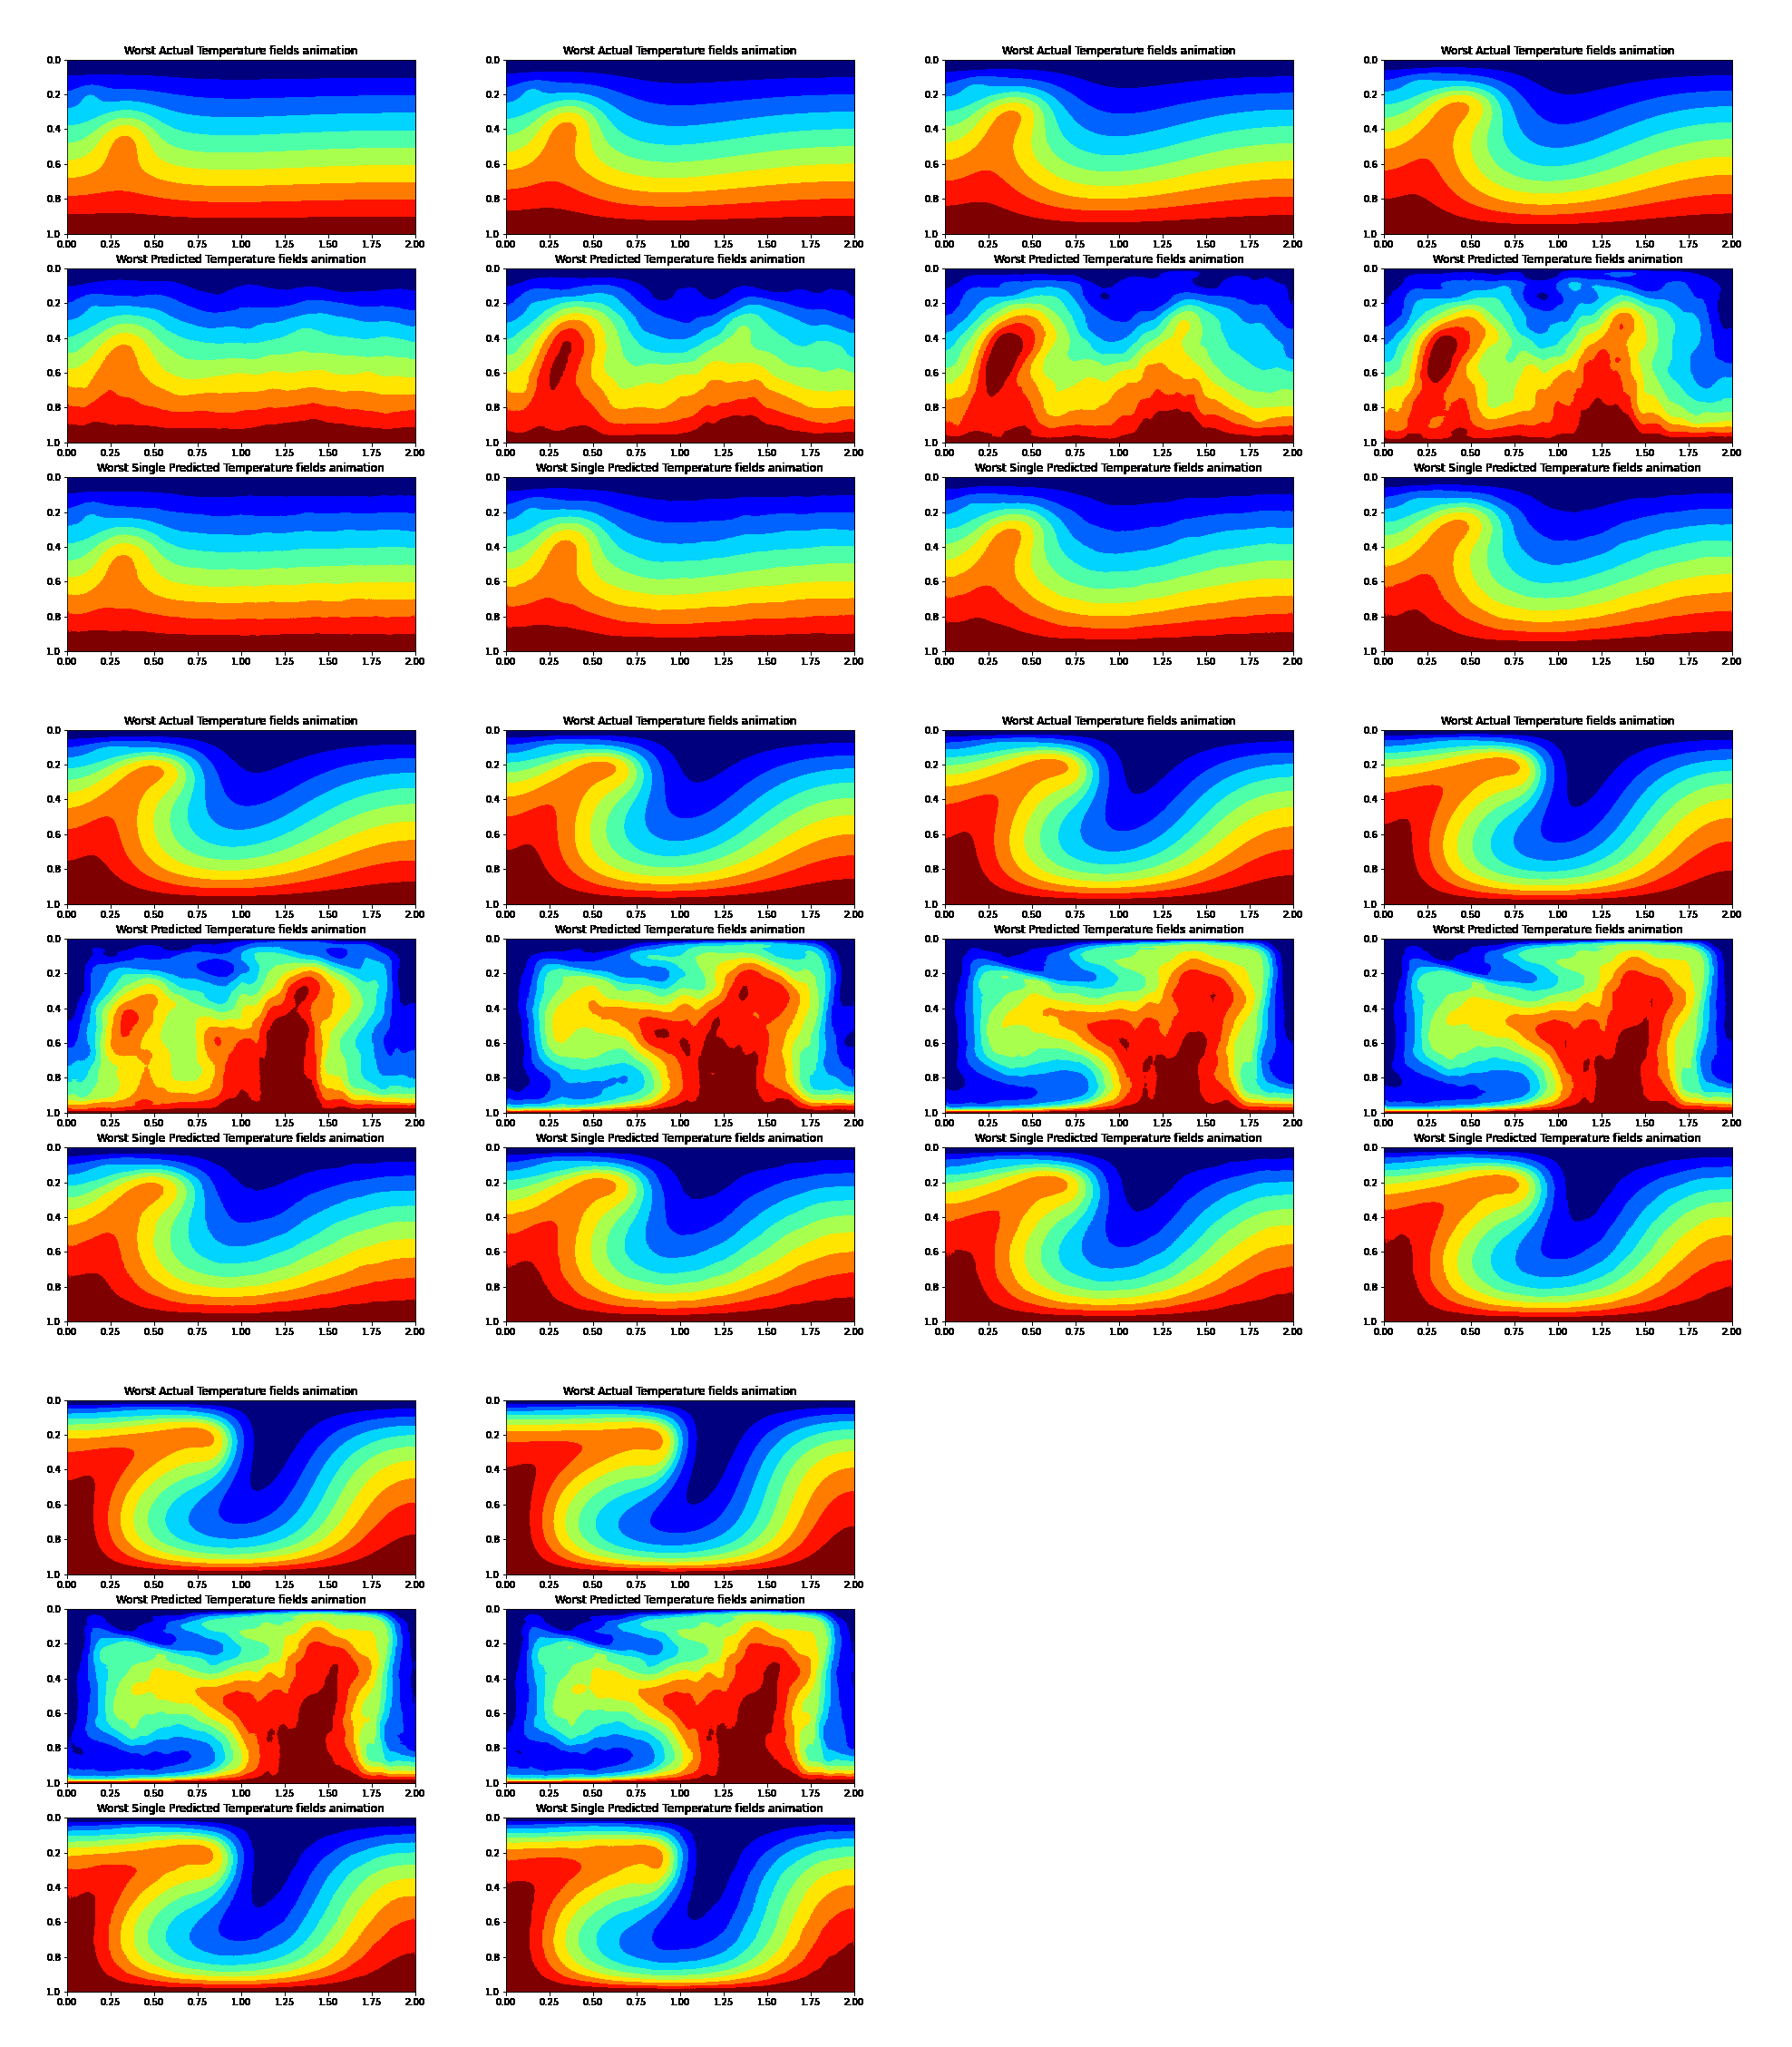
\includegraphics[scale=0.10]{figures/mantle_convection_images/limited_dataset/FNN_Worst_GIF_sheet.png}
    \label{figure:FNN_limited_worst_gif}
\end{figure}

To further evaluate the performance of these two methods, we applied a technique called Proper Orthogonal Decomposition (POD) to the set of predictions generated by these two methods in both the best case and the worst case, along with the original time series and the compressed-decompressed version generated by ConvAE serve as contrast.

POD is mainly used to decompose a physical field (e.g. temperature field) depending on the different variables that influence its physical behaviors and it is similar to Principle Component Analysis (PCA) since it refers to eigenvalues of a physical field.\citep{10.1146_annurev.fl.25.010193.002543} Following \citep{10.1515_9783110671490-007}, the Singular Value Decomposition (SVD) of a simulation matrix $X$ (spatial points × time-steps, in this case it's $201 \times 401 \times 100$) is computed as:

\begin{equation}
X = U\Sigma V
\end{equation}

where the diagonal of $\Sigma$ contains the eigenvalues (POD coefficient) for this simulation.

Figure \ref{figure:FNN_limited_best_POD} and Figure \ref{figure:FNN_limited_worst_POD} show the POD result in the best case and the worst case:

\begin{figure}[H]
    \caption{Best case POD of FNN trained with Limited Dataset.}
    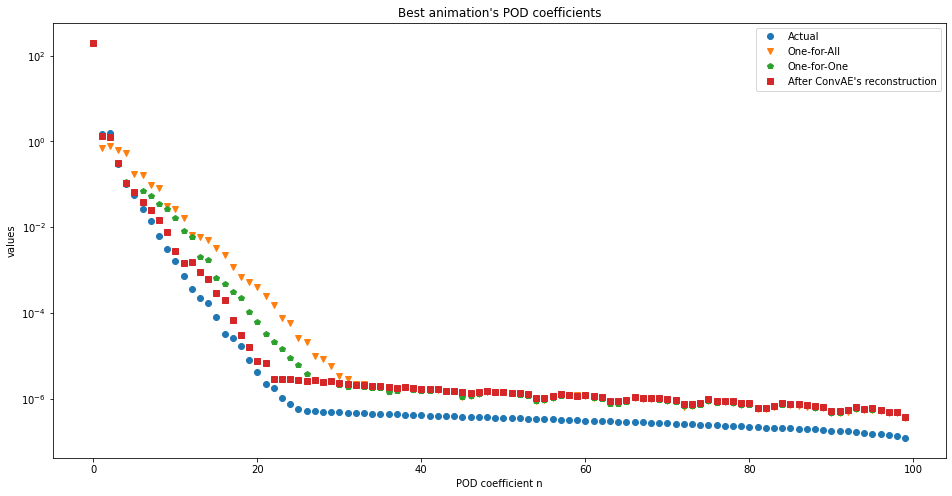
\includegraphics[scale=0.5]{figures/mantle_convection_images/limited_dataset/FNN_Best_POD.png}
    \label{figure:FNN_limited_best_POD}
\end{figure}

\begin{figure}[H]
    \caption{Worst case POD of FNN trained with Limited Dataset.}
    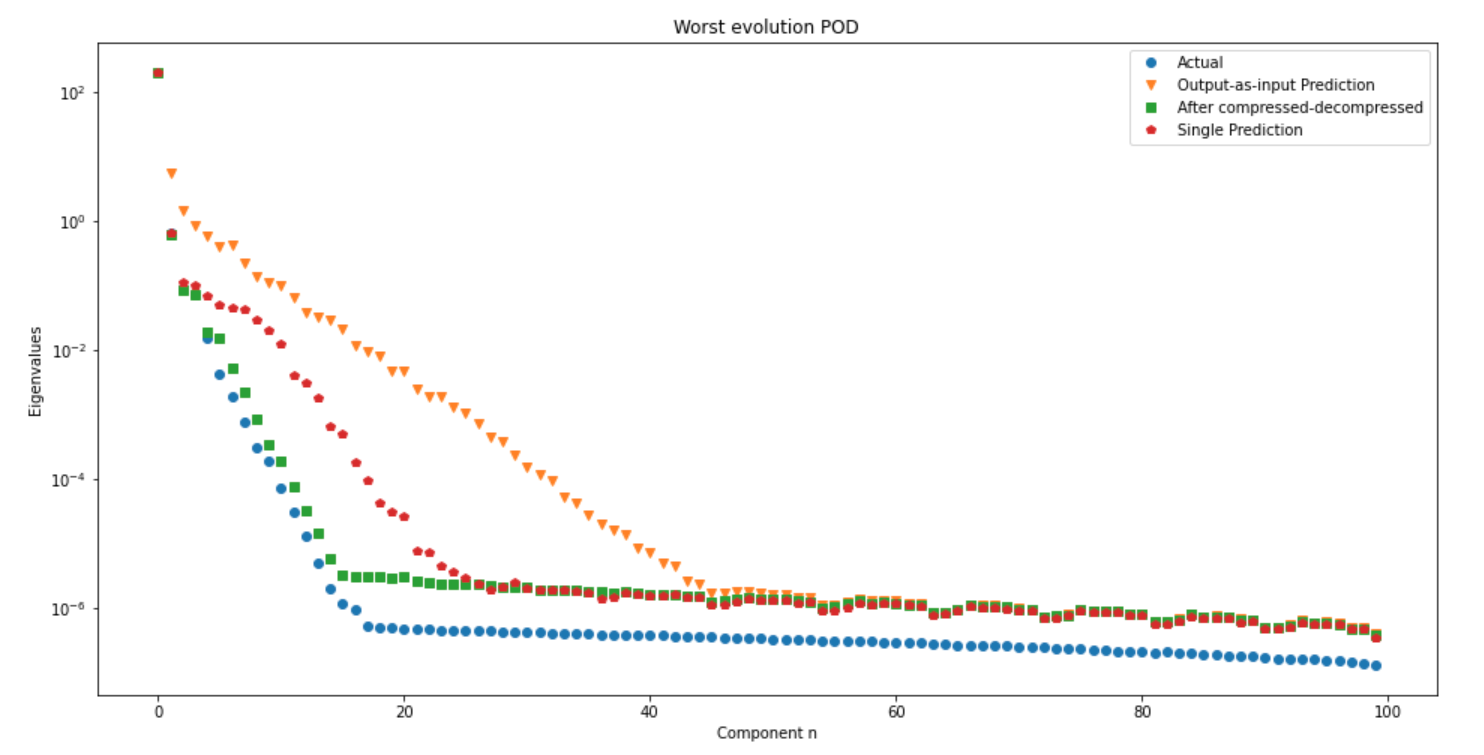
\includegraphics[scale=0.5]{figures/mantle_convection_images/limited_dataset/FNN_Worst_POD.png}
    \label{figure:FNN_limited_worst_POD}
\end{figure}

As seen in the animations and the POD results, the first method (output-as-input prediction) fails to capture the trend of the temperature fields simulations in the worst case and the result prediction is completely different to the actual simulations. This is because the information loss from the ConvAE and FNN in each prediction-as-input loop accumulates, leading to poor result after 99 iterations. In the mean time, the prediction result for the second method mostly matches with the actual output in both cases, which is consistent to our theory that the it is the first method itself leads to the huge information loss.

Also, the predicted GIFs in this case are either moving faster or slower than the actual simulation. This is probably due to the varying distance between time steps in the simulation. In this case, the model will try to predict the temperature field at the next time step by averaging out the distance between each time step, thus making the predicted simulations either too fast or too slow.

To explore if we can generate a sequence of temperature fields with less information loss, we try to use LSTM to predict the latent space representation instead.


\subsection{Long Short-Term Memory (LSTM) for Prediction}

We now move on to predict a sequence of latent space representation using LSTM. The LSTM in this study uses the first 50 temperature fields as a sequence in each file as one training set, takes a sequence of 50 temperature fields as the input and output the rest 50 temperature fields at the next time steps.

This 50:50 of input-output length is determined by PyTorch's technical limitation on LSTM, where the input length and the output length should be the same for the LSTM to functionally work. A ratio of less input length and more output length (20:80) had been considered, but this requires the input sequence to be replicated into 4 times the size to match with PyTorch's requirement, which could lead to worse prediction result compared with the 50:50 ratio.

Therefore, the files in the dataset are randomly shuffled and divided in a ratio of 80\%, 10\%, 10\% for training, testing and validation where each piece of data is a complete file to be divided in half as input and output.

Again, before a sequence of latent space representation is fed as the input of LSTM, it is flattened into two dimension ($50 \times 6210$). The prediction of LSTM in this case is then resized from $50 \times 6210$ to $50 \times 6 \times 23 \times 45$ for the convenience of further testing.

The learnable parameters of LSTM are optimized using small mini-batches (only 1 batch in this case since we have merely 80 training samples) and Adam as the optimizer, where the loss function is defined as the MSE between the prediction of LSTM and the actual output (both in the shape of a sequence of latent space representation, which is $50 \times 6 \times 23 \times 45$).

After testing with LSTMs that have different architectures, we found that architectures with a total number of 2 consecutive LSTM layers perform the best. (We also test some deeper architectures with 4-6 LSTM. However, there is no significant reduction in the loss value)

In the following figures, we present results from an architecture with 2 LSTM layers (first one input size is 6210, hidden size is 3105; second one input size is 3105, hidden size is 6210. Both of them only have one layer, no internal stacking), and trained for 200 epochs. The figures include the training loss and validation loss from Figure \ref{figure:LSTM_limited_losses}, overall testing result from Figure \ref{figure:LSTM_limited_testing}, and the most/least accurate prediction in Figure \ref{figure:LSTM_limited_best} and Figure \ref{figure:LSTM_limited_worst}:

\begin{figure}[H]
    \caption{Training loss and Validation loss of LSTM trained with Limited Dataset.}
    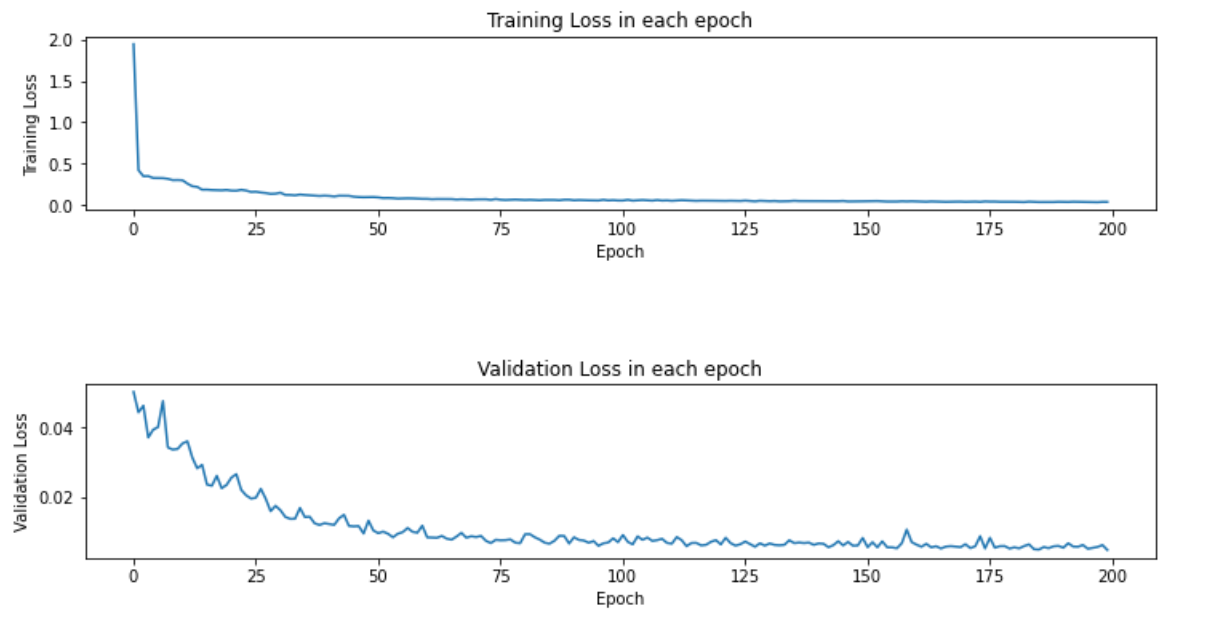
\includegraphics[scale=0.6]{figures/mantle_convection_images/limited_dataset/LSTM_trainingData.png}
    \label{figure:LSTM_limited_losses}
\end{figure}

\begin{figure}[H]
    \caption{Overall testing result of LSTM trained with Limited Dataset.}
    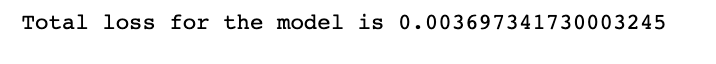
\includegraphics[scale=0.8]{figures/mantle_convection_images/limited_dataset/LSTM_OverallTesting.png}
    \label{figure:LSTM_limited_testing}
\end{figure}

\begin{figure}[H]
    \caption{Ground truth, ground truth after ConvAE's compression-decompression, and most accurate prediction of LSTM trained with Limited Dataset.}
    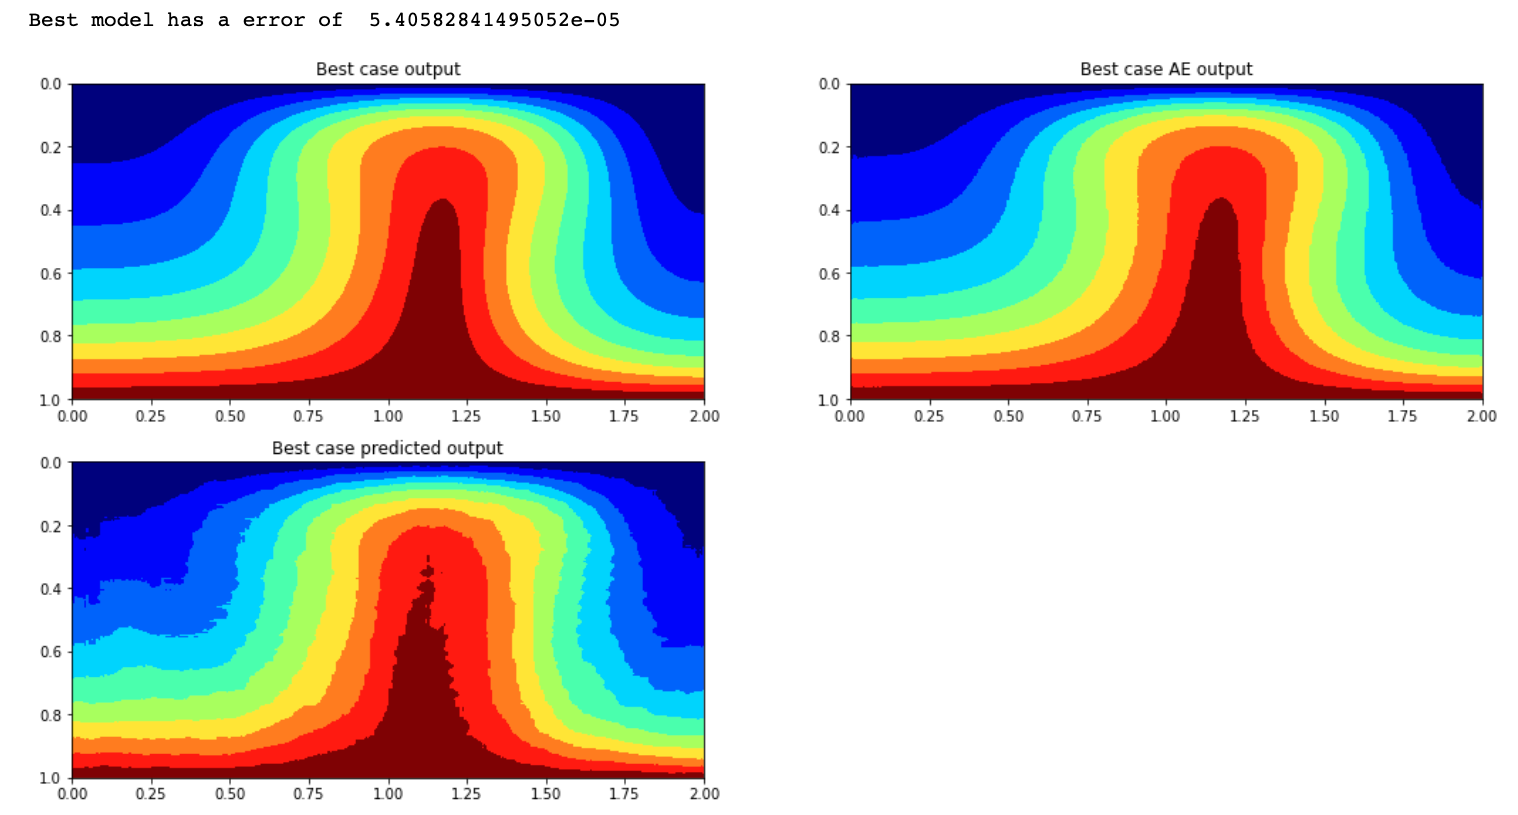
\includegraphics[scale=0.5]{figures/mantle_convection_images/limited_dataset/LSTM_Best.png}
    \label{figure:LSTM_limited_best}
\end{figure}

\begin{figure}[H]
    \caption{Ground truth, ground truth after ConvAE's compression-decompression, and least accurate prediction of LSTM trained with Limited Dataset.}
    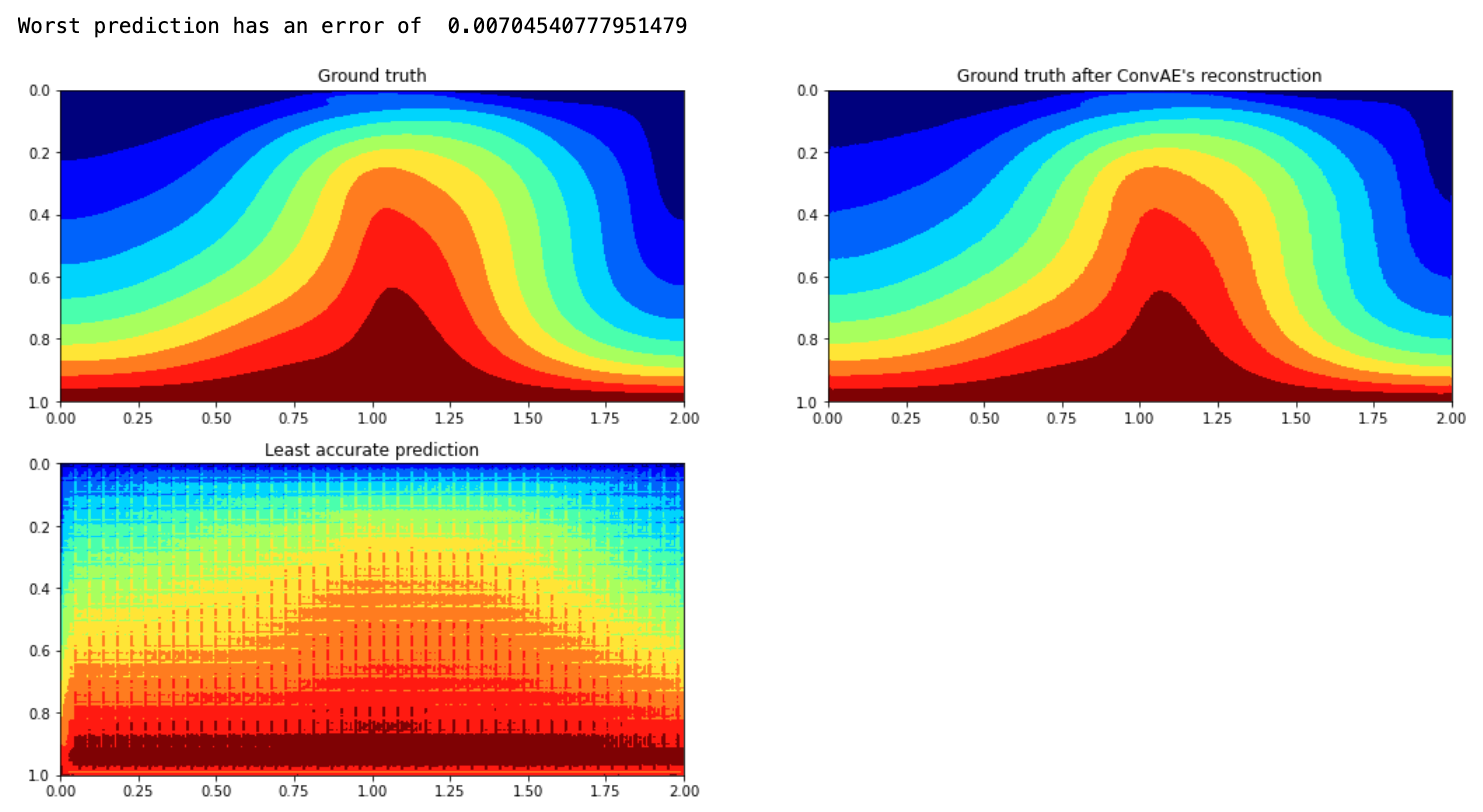
\includegraphics[scale=0.5]{figures/mantle_convection_images/limited_dataset/LSTM_Worst.png}
    \label{figure:LSTM_limited_worst}
\end{figure}

On average, the loss values are higher than the FNN and no overfitting occurs. The prediction is able to capture the main features precisely with some small information loss in the best case, but fails to do so in the worst case. This is caused by the internal structure of LSTM since the worst case is the first temperature field in the output sequence.

To better visualize the prediction result of LSTM on a 50:50 input length to output length ratio, two animations representing the best case and the worst case (evaluated based on the sum of MSE for each predicted temperature in the output sequence) in the format of GIF files are generated. From top to bottom, the first picture represents the actual output from the dataset and the second one represents the prediction result.

Figure \ref{figure:LSTM_limited_best_gif} and Figure \ref{figure:LSTM_limited_worst_gif} show 20\% of the two sprite sheets converted from the original GIFs (Every 5th frame) for the convenience of reading:

\begin{figure}[H]
    \centering
    \caption{Best case animation sheet of LSTM trained with Limited Dataset (Link to this GIF: \url{https://drive.google.com/file/d/1zNJrZUB8XBAEWsUHPd2NANuWkE8yNg3z/view?usp=sharing})}
    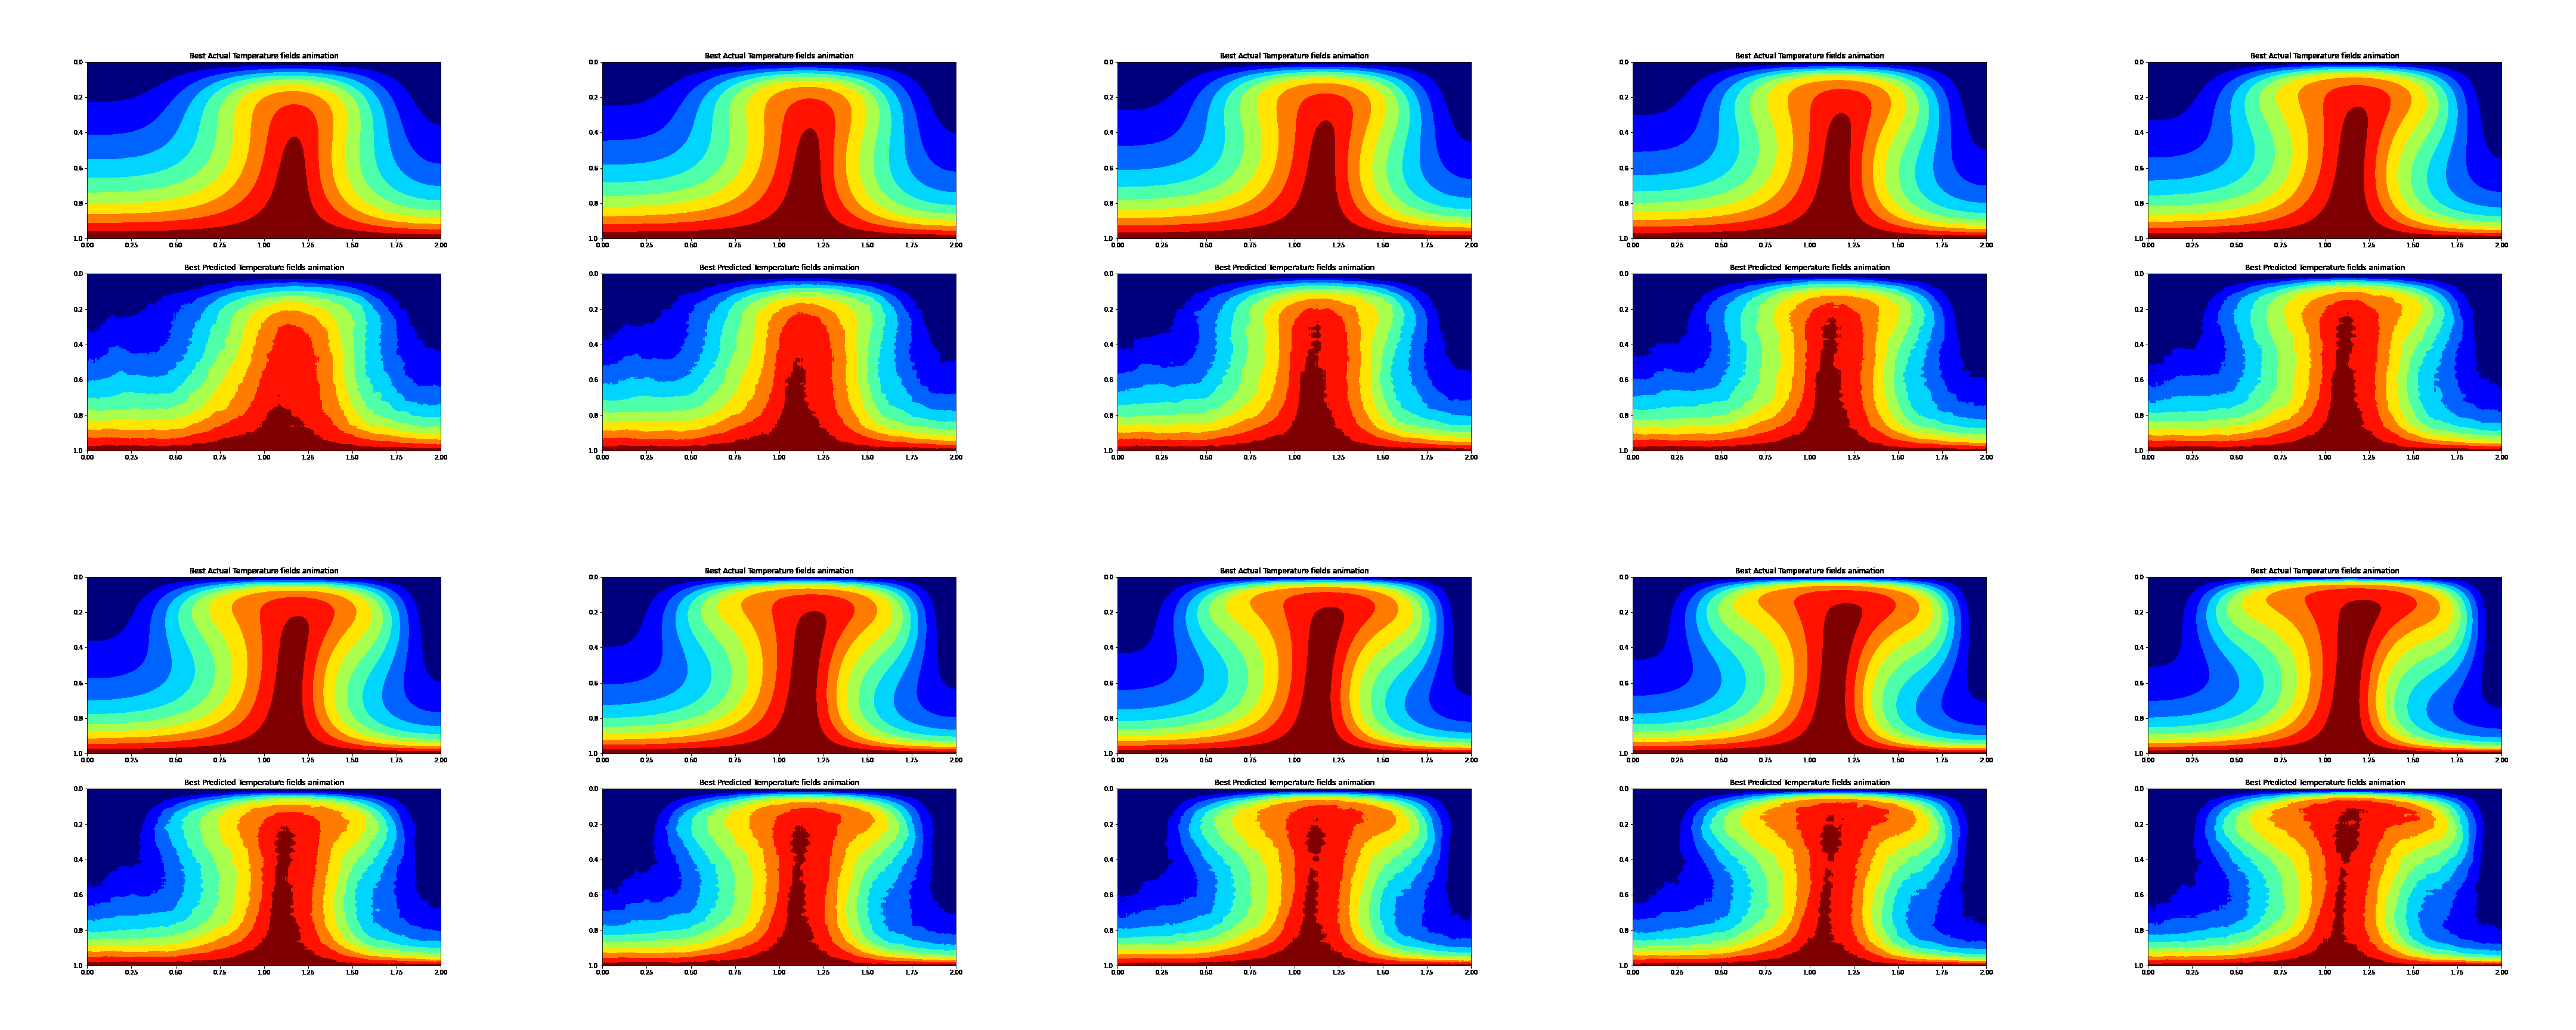
\includegraphics[scale=0.10]{figures/mantle_convection_images/limited_dataset/LSTM_Best_GIF_sheet.png}
    \label{figure:LSTM_limited_best_gif}
\end{figure}



\begin{figure}[H]
    \centering
    \caption{Worst case animation sheet of LSTM trained with Limited Dataset (Link to this GIF: 
    \url{https://drive.google.com/file/d/1nINRk2Oh8rgQBLWio_b6R6I7T18e7Zi-/view?usp=sharing})}
    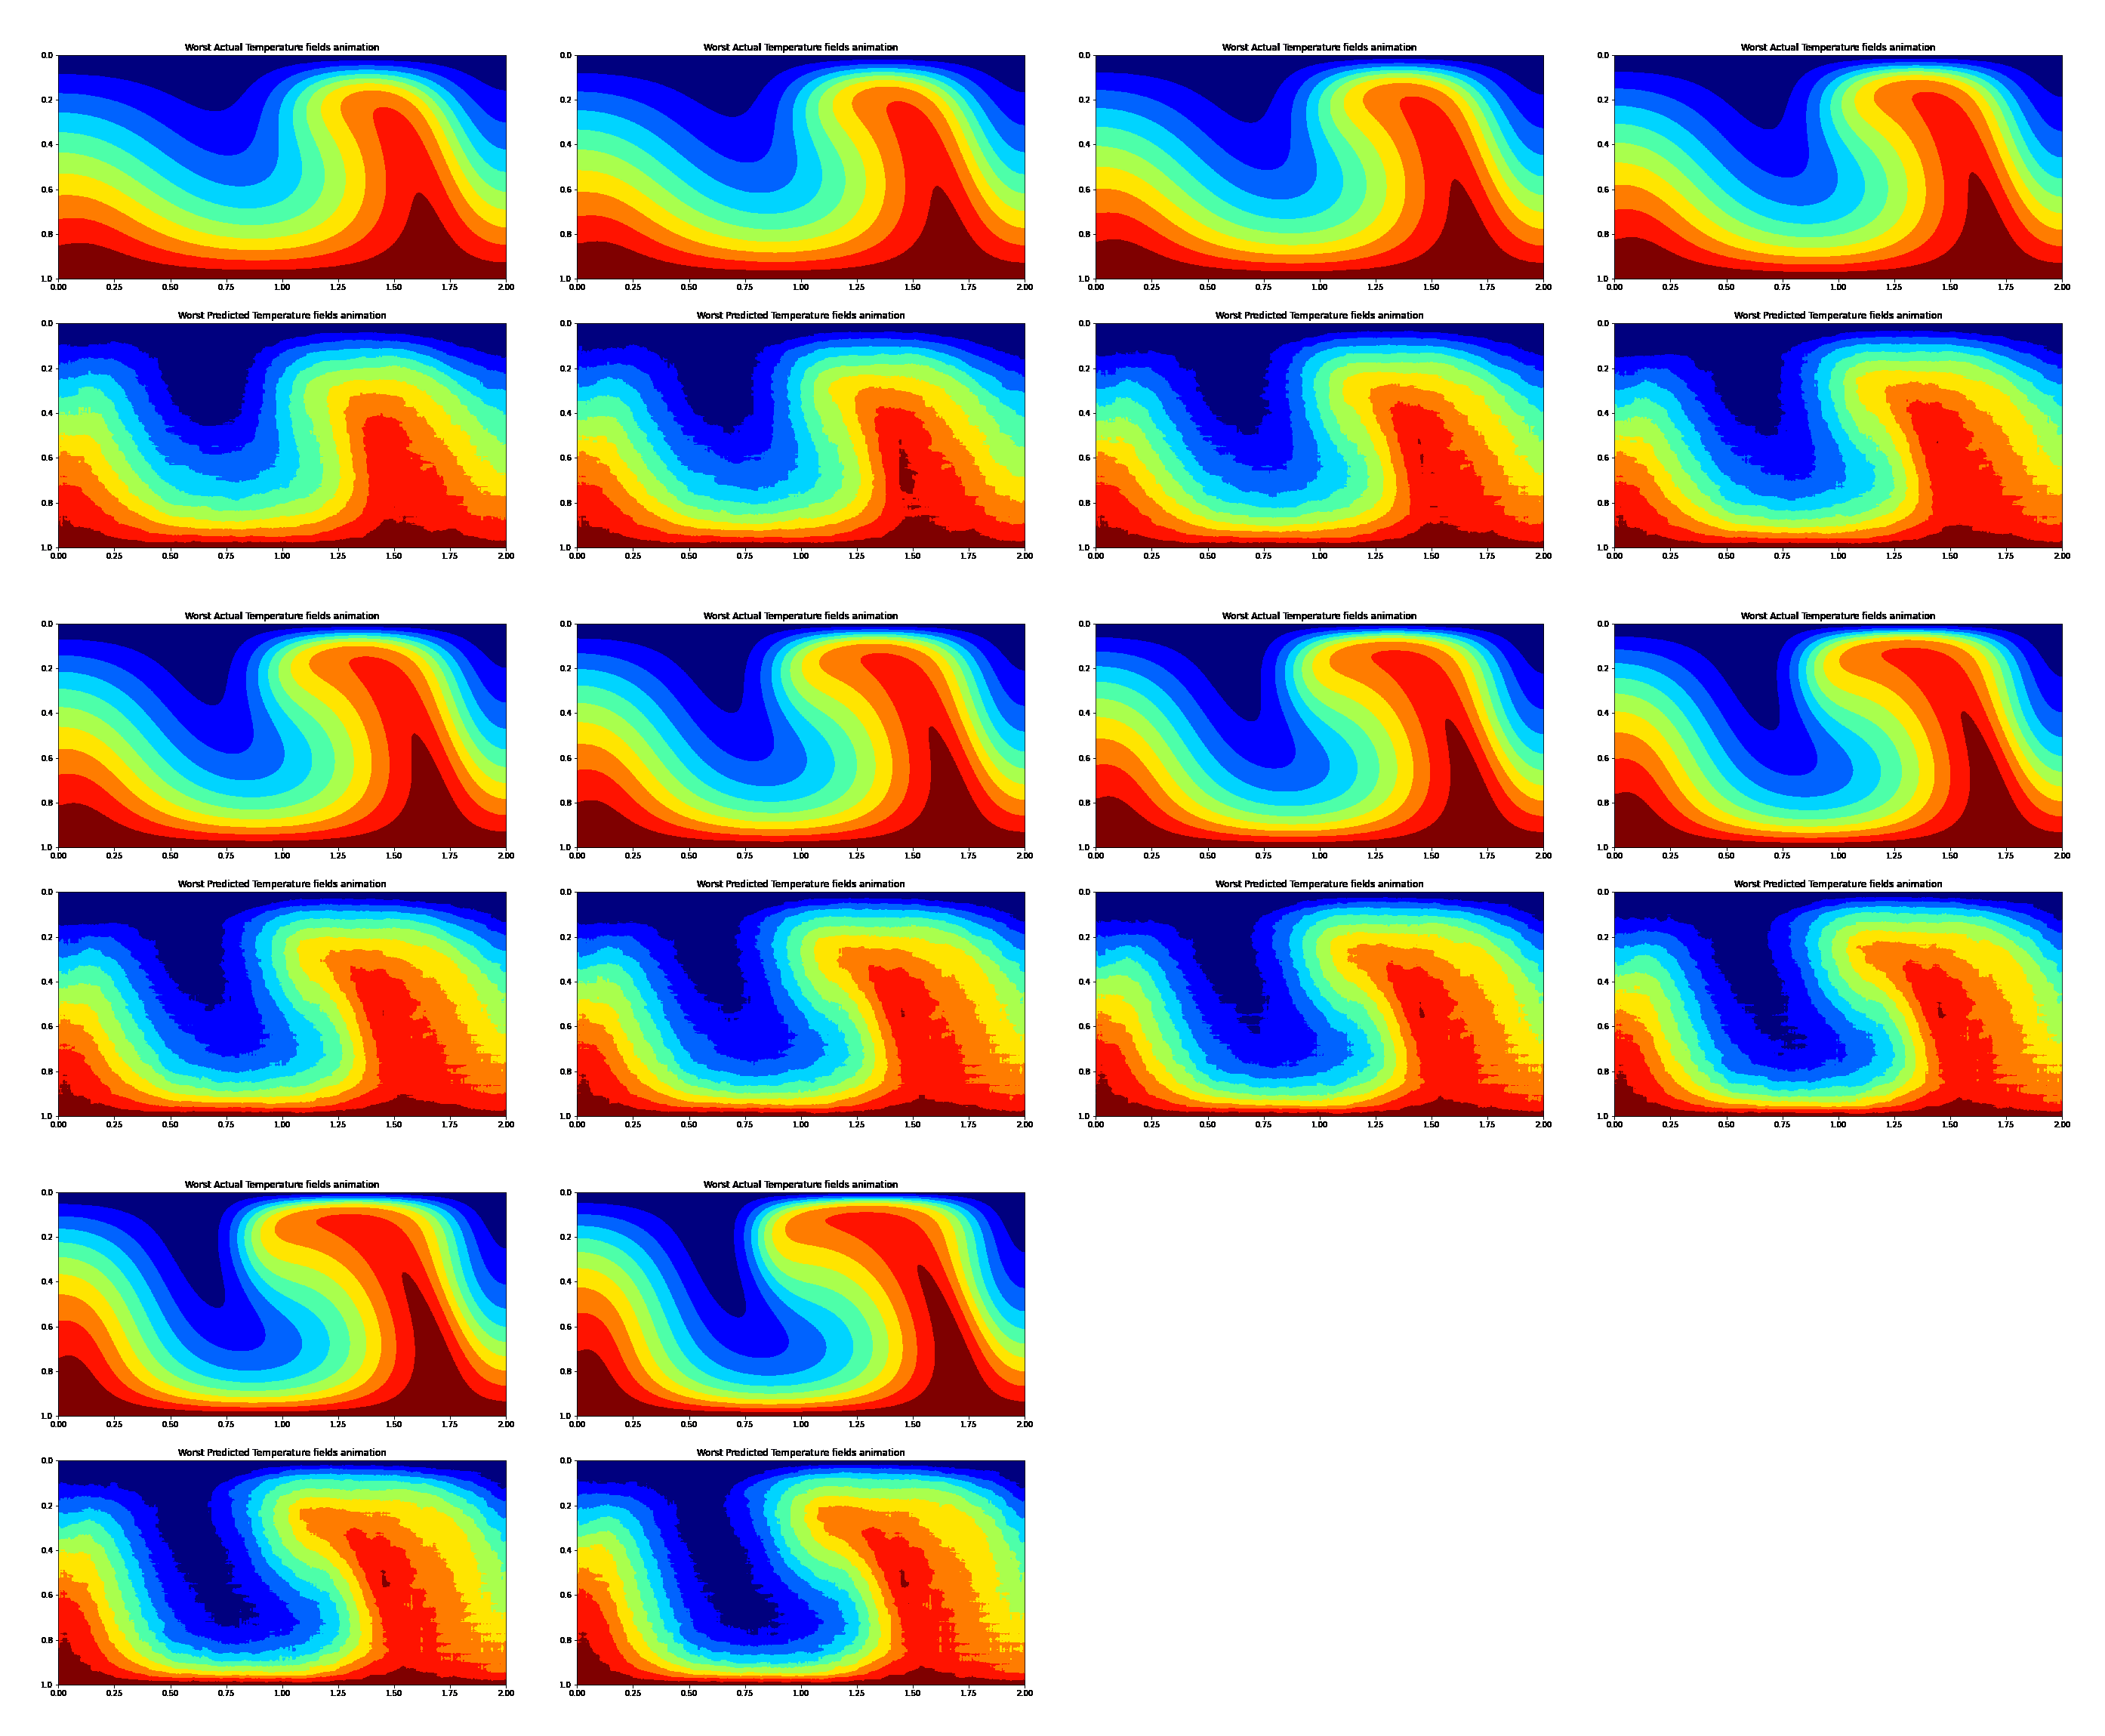
\includegraphics[scale=0.10]{figures/mantle_convection_images/limited_dataset/LSTM_Worst_GIF_sheet.png}
    \label{figure:LSTM_limited_worst_gif}
\end{figure}

To further evaluate the performance, we also applied POD to a sequence of predictions generated by LSTM in both the best case and the worst case, with the original time series and the compressed-decompressed version generated by ConvAE serving as contrast.

Figure \ref{figure:LSTM_limited_best_POD} and Figure \ref{figure:LSTM_limited_worst_POD} show the POD result in best case and the worst case:

\begin{figure}[H]
    \caption{Best case POD of LSTM trained with Limited Dataset.}
    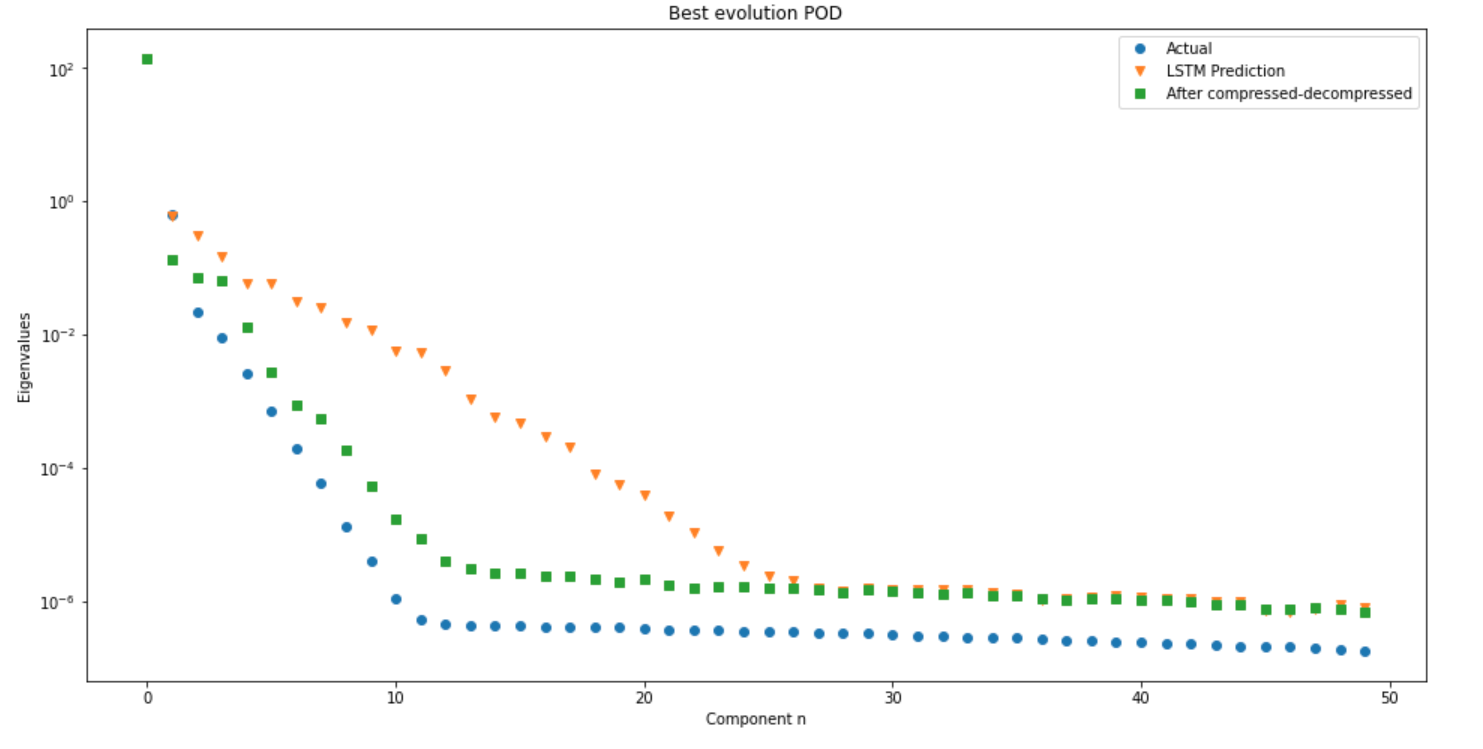
\includegraphics[scale=0.5]{figures/mantle_convection_images/limited_dataset/LSTM_Best_POD.png}
    \label{figure:LSTM_limited_best_POD}
\end{figure}

\begin{figure}[H]
    \caption{Worst case POD of LSTM trained with Limited Dataset.}
    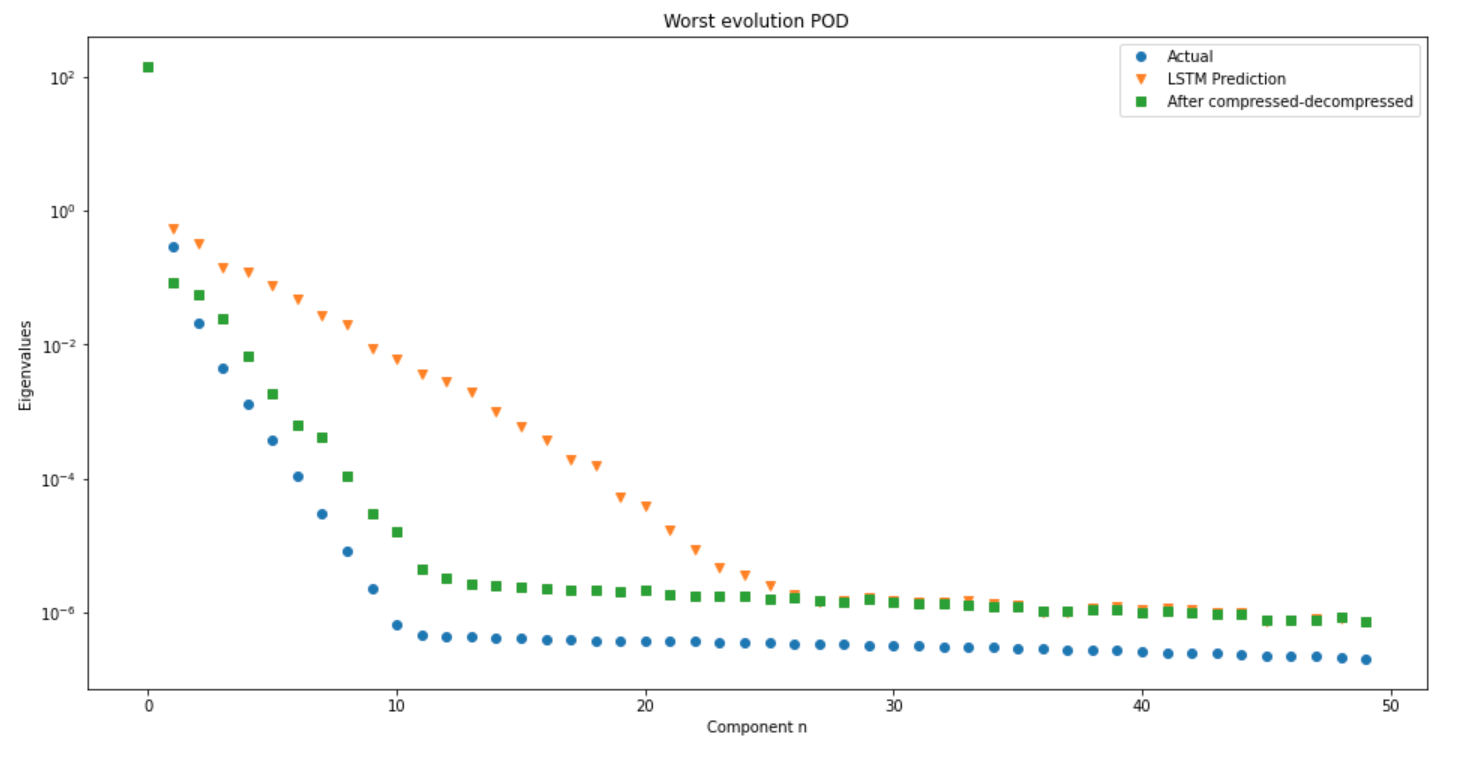
\includegraphics[scale=0.5]{figures/mantle_convection_images/limited_dataset/LSTM_Worst_POD.png}
    \label{figure:LSTM_limited_worst_POD}
\end{figure}

From the animations and the POD results, we can conclude that LSTM is able to capture the characteristics of the simulations even in its worst case. However, the simulations predicted using LSTM are less accurate and have more data loss compared with those predicted using FNN. There could be potential underfitting problem due to the lack of training data since only 80 samples are used for training.


\section{Mantle Convection Simulation on Larger Dataset}

To confirm if the low accuracy of LSTM is caused by the scarceness of data, a larger dataset is tested, whose only two differences with the limited dataset are that it now contains 903 simulations and it uses absolute time steps instead of adaptive time steps. However, even though it now uses absolute time steps, the distance between each of the consecutive time steps still varies.

For this section, the distance between time steps are not considered since we want to mainly focus on testing if the scarceness of data is the reason for the low accuracy of LSTM. Nevertheless, time steps will be used in the next section to create an interpolated dataset.

The larger dataset are randomly divided in the same way as the limited dataset for each of the three ML architectures in the following subsections.

\subsection{Compression of temperature fields}

The ConvAE used for compressing the temperature fields in this section has the same structure and the same set of hyperparamters as the one trained with limited dataset, except that the total number of epochs are now reduced from 1000 to 200 due to the constrains of the computation resources on Gadi.

In the following figures, some detailed test results from this ConvAE trained with larger dataset are presented, including the training loss and validation loss from Figure \ref{figure:ConvAE_larger_losses}, overall testing result from Figure \ref{figure:ConvAE_larger_testing}, and the most/least accurate prediction in Figure \ref{figure:ConvAE_larger_best_worst}:
:

\begin{figure}[H]
    \caption{Training loss and Validation loss of ConvAE trained with Larger Dataset.}
    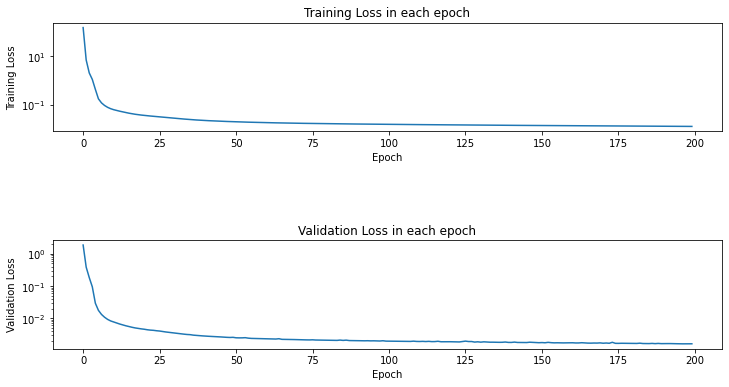
\includegraphics[scale=0.6]{figures/mantle_convection_images/larger_dataset/ConvAE_trainingData.png}
    \label{figure:ConvAE_larger_losses}
\end{figure}

\begin{figure}[H]
    \caption{Overall testing result of ConvAE trained with Larger Dataset.}
    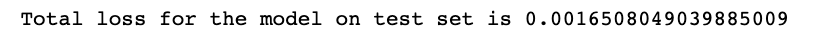
\includegraphics[scale=0.8]{figures/mantle_convection_images/larger_dataset/ConvAE_OverallTesting.png}
    \label{figure:ConvAE_larger_testing}
\end{figure}

\begin{figure}[H]
\centering
\begin{subfigure}{0.45\textwidth}
    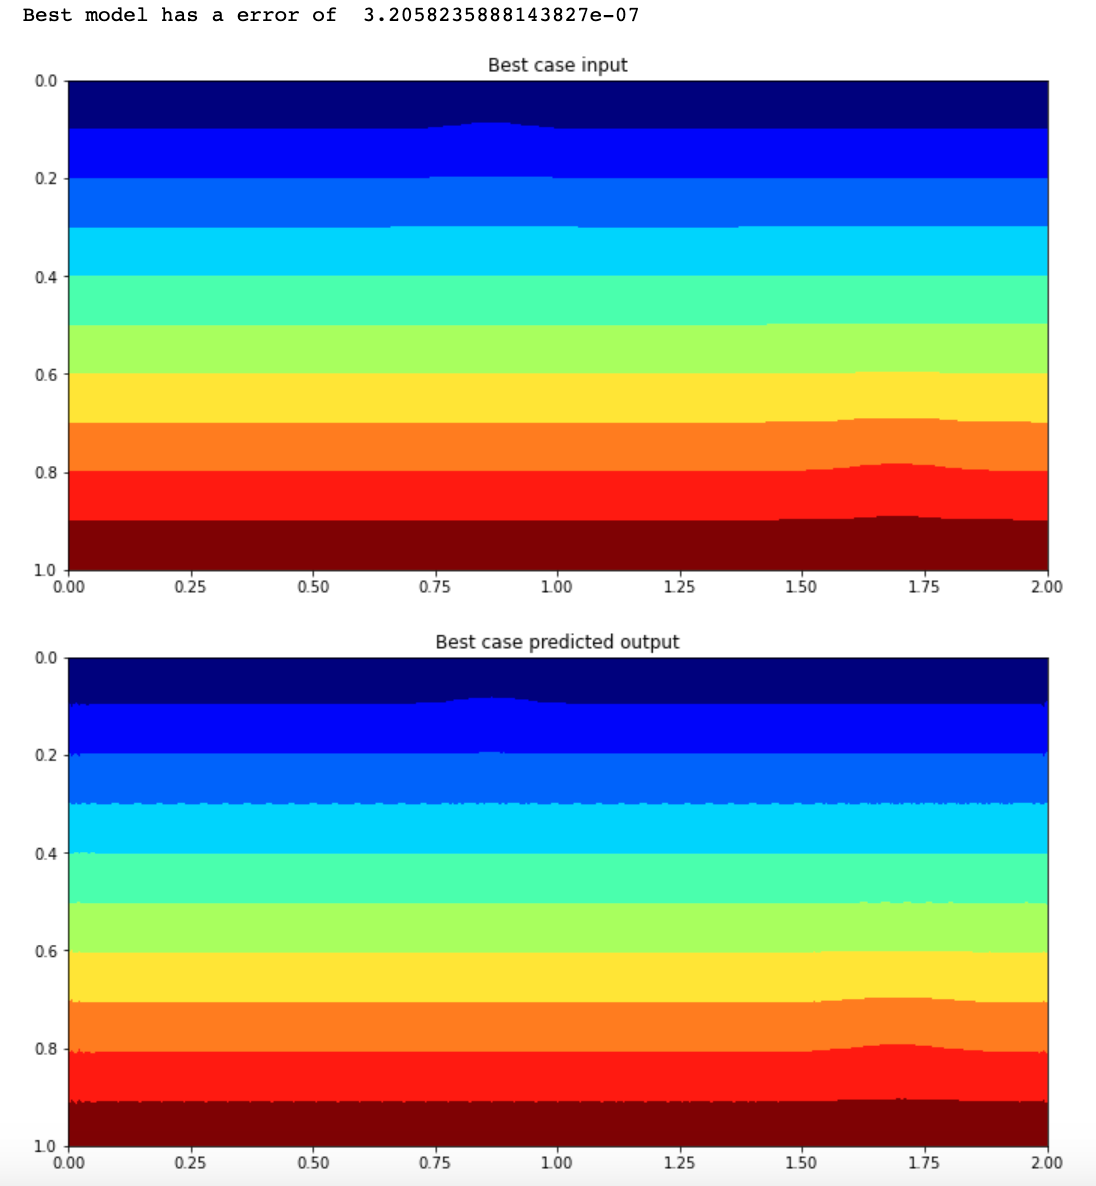
\includegraphics[width=\textwidth]{figures/mantle_convection_images/larger_dataset/ConvAE_Best.png}
    \caption{Most accurate reconstruction of ConvAE trained with Larger Dataset.}
\end{subfigure}
\hfill
\begin{subfigure}{0.45\textwidth}
    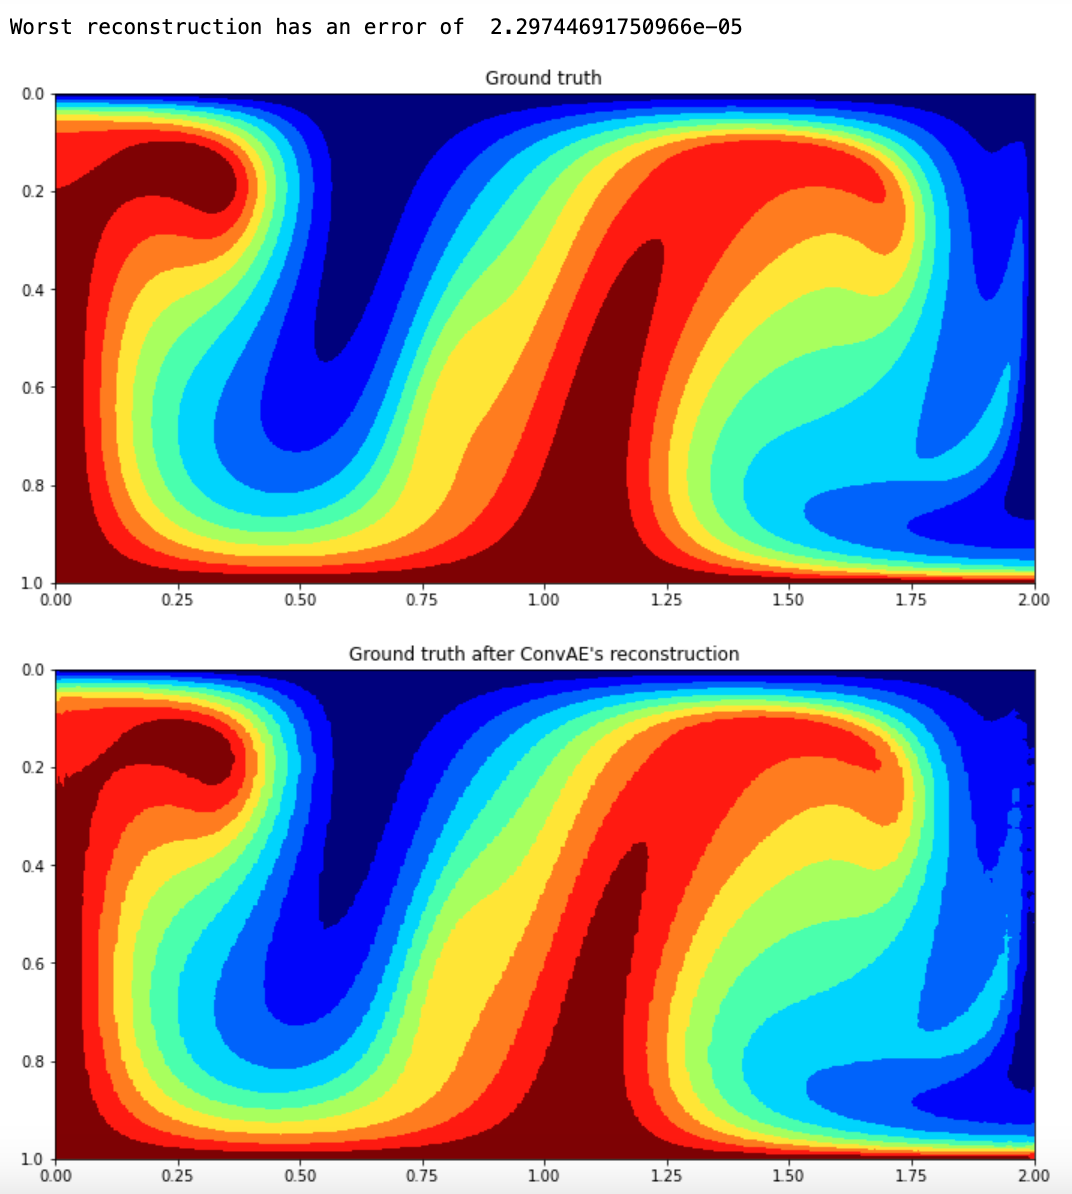
\includegraphics[width=\textwidth]{figures/mantle_convection_images/larger_dataset/ConvAE_Worst.png}
    \caption{Least accurate reconstruction of ConvAE trained with Larger Dataset.}
\end{subfigure}   
\caption{Best case and worst case using ConvAE.}
\label{figure:ConvAE_larger_best_worst}
\end{figure}

Overall, the performance of this ConvAE is similar to the one trained with limited dataset: reconstruction loss are low and no overfitting occurs.


\subsection{Fully Connected Neural Network for Prediction}

The FNN in this section also has the same structure and the same set of hyperparamters as the one trained with limited dataset, except that the total number of epochs are reduced from 1000 to 200 as well.

The results are presented in the following figures, including the training loss and validation loss from Figure \ref{figure:FNN_larger_losses}, overall testing result from Figure \ref{figure:FNN_larger_testing}, and the most/least accurate prediction in Figure \ref{figure:FNN_larger_best} and Figure \ref{figure:FNN_larger_worst}:

\begin{figure}[H]
    \caption{Training loss and Validation loss of FNN trained with Larger Dataset.}
    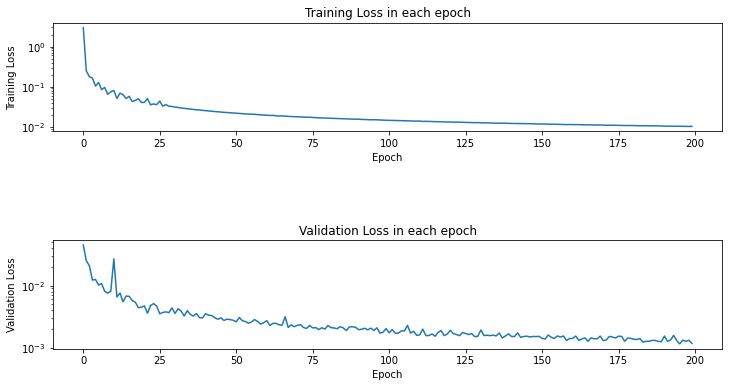
\includegraphics[scale=0.6]{figures/mantle_convection_images/larger_dataset/FNN_trainingData.png}
    \label{figure:FNN_larger_losses}
\end{figure}

\begin{figure}[H]
    \caption{Overall testing result of FNN trained with Larger Dataset.}
    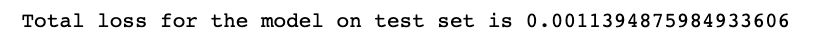
\includegraphics[scale=0.8]{figures/mantle_convection_images/larger_dataset/FNN_OverallTesting.png}
    \label{figure:FNN_larger_testing}
\end{figure}

\begin{figure}[H]
    \caption{Ground truth, ground truth after ConvAE's compression-decompression, and most accurate prediction of FNN trained with Larger Dataset.}
    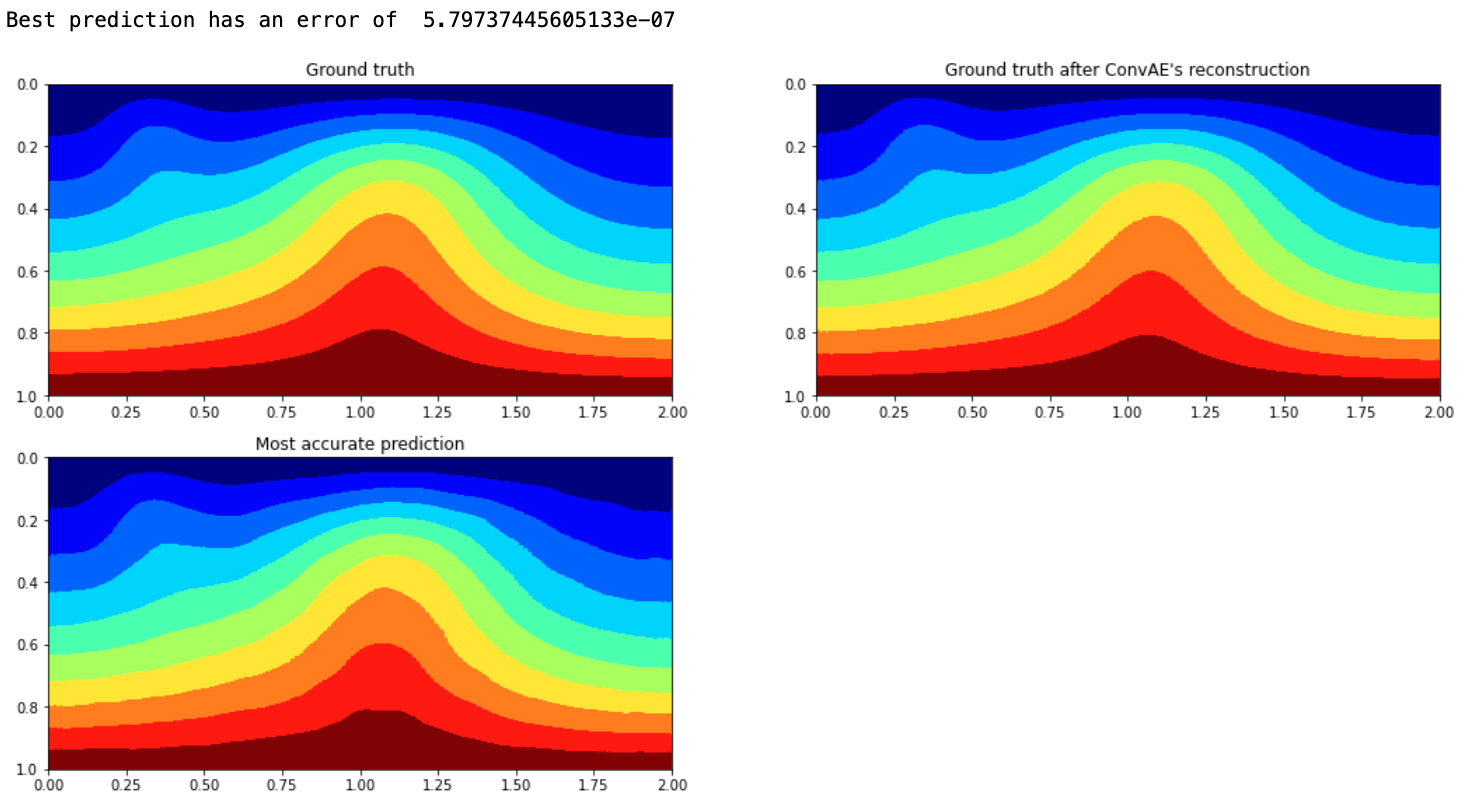
\includegraphics[scale=0.5]{figures/mantle_convection_images/larger_dataset/FNN_Best.png}
    \label{figure:FNN_larger_best}
\end{figure}

\begin{figure}[H]
    \caption{Ground truth, ground truth after ConvAE's compression-decompression, and least accurate prediction of FNN trained with Larger Dataset.}
    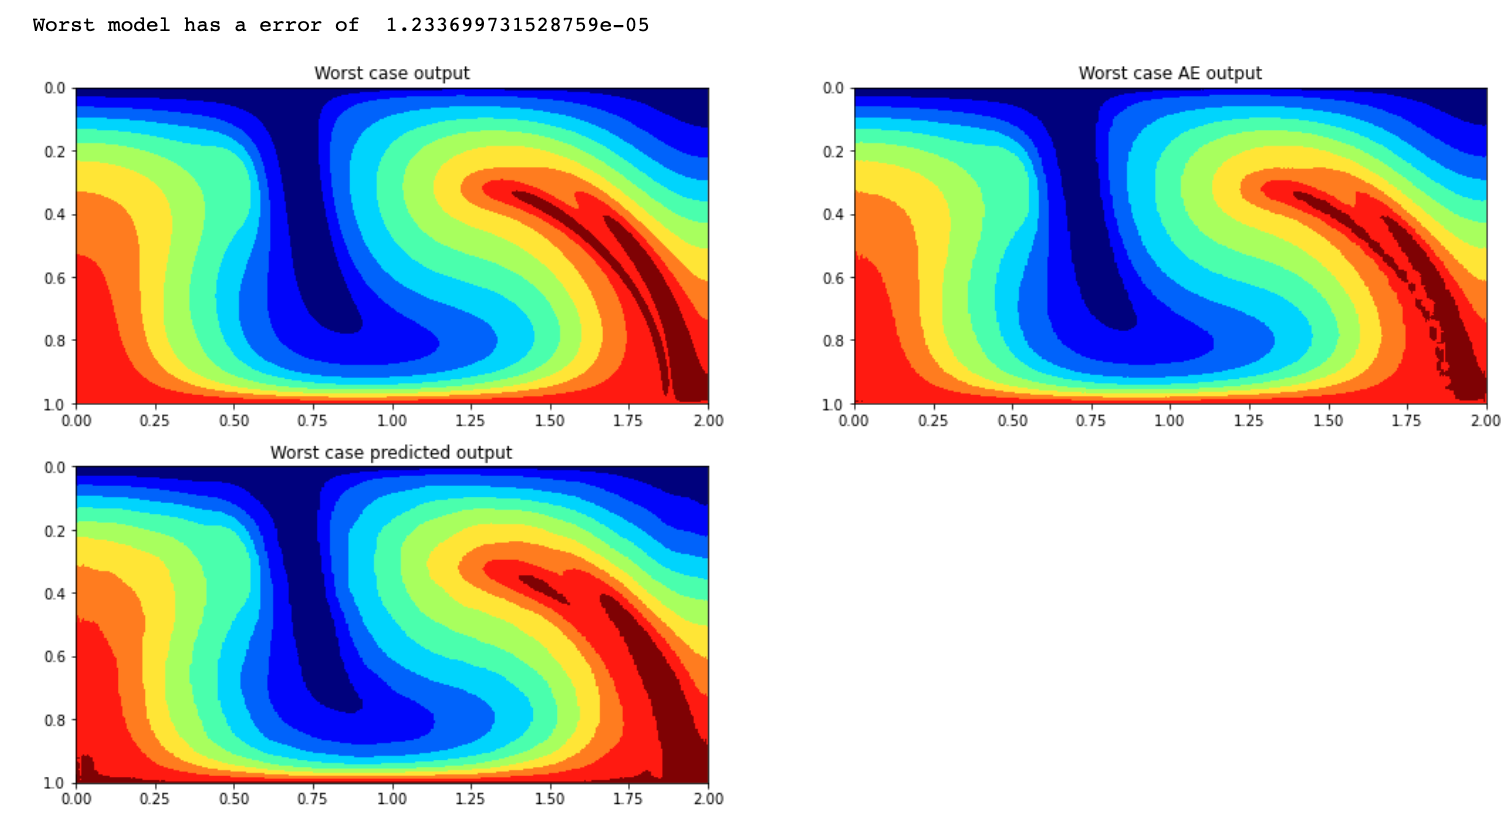
\includegraphics[scale=0.5]{figures/mantle_convection_images/larger_dataset/FNN_Worst.png}
    \label{figure:FNN_larger_worst}
\end{figure}

The above result of this FNN are similar to the one trained with limited dataset: the loss values are low and no overfitting occurs. There are still some small information loss, which is now confirmed as caused by the loss of data generated during the compression-decompression process of ConvAE.

Again, two animations representing the best case and the worst case when predicting the entire simulation using "One-for-All" (use $T1$ from dataset $\rightarrow$ get predicted $T2$ $\rightarrow$ use predicted $T2$ $\rightarrow$ get predicted $T3$ $\rightarrow$ ...) are generated.

Figure \ref{figure:FNN_larger_best_gif} and Figure \ref{figure:FNN_larger_worst_gif} show 10\% of the two sprite sheets converted from the original GIF animations (Every 10th frame).

\begin{figure}[H]
    \centering
    \caption{Best case animation sheet of FNN trained with Larger Dataset (Link to this GIF: \url{https://drive.google.com/file/d/1LxuwXxEoG5xsYzLYn6n6-mUfoP8A3IC2/view?usp=sharing})}
    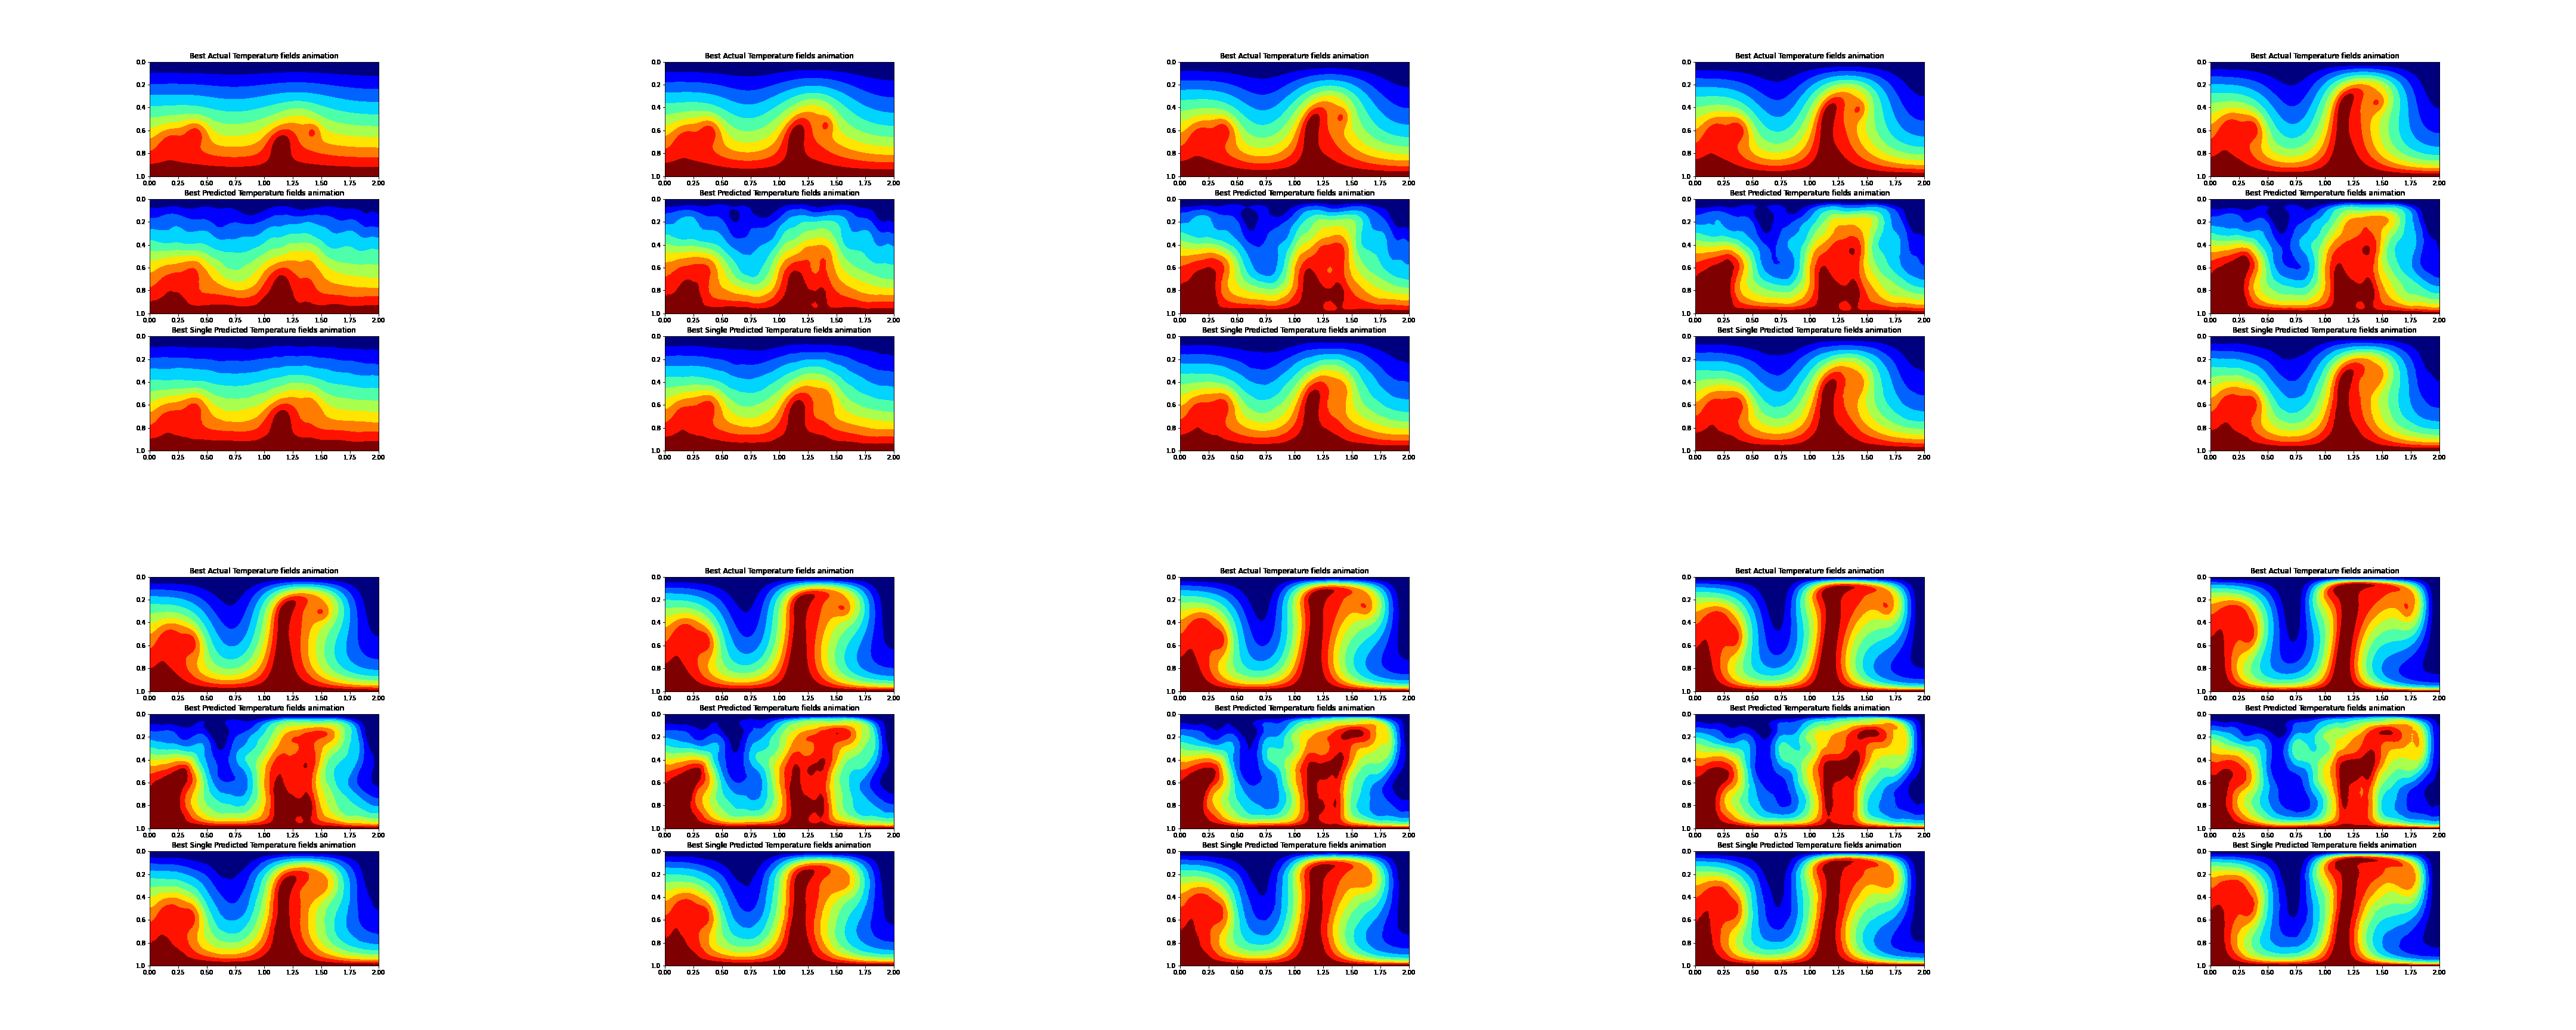
\includegraphics[scale=0.10]{figures/mantle_convection_images/larger_dataset/FNN_Best_GIF_sheet.png}
    \label{figure:FNN_larger_best_gif}
\end{figure}

\begin{figure}[H]
    \centering
    \caption{Worst case animation sheet of FNN trained with Larger Dataset (Link to this GIF: 
    \url{https://drive.google.com/file/d/1vwfL_n6ANnkJEY3B8a024SF_yQ35Hkxu/view?usp=sharing})}
    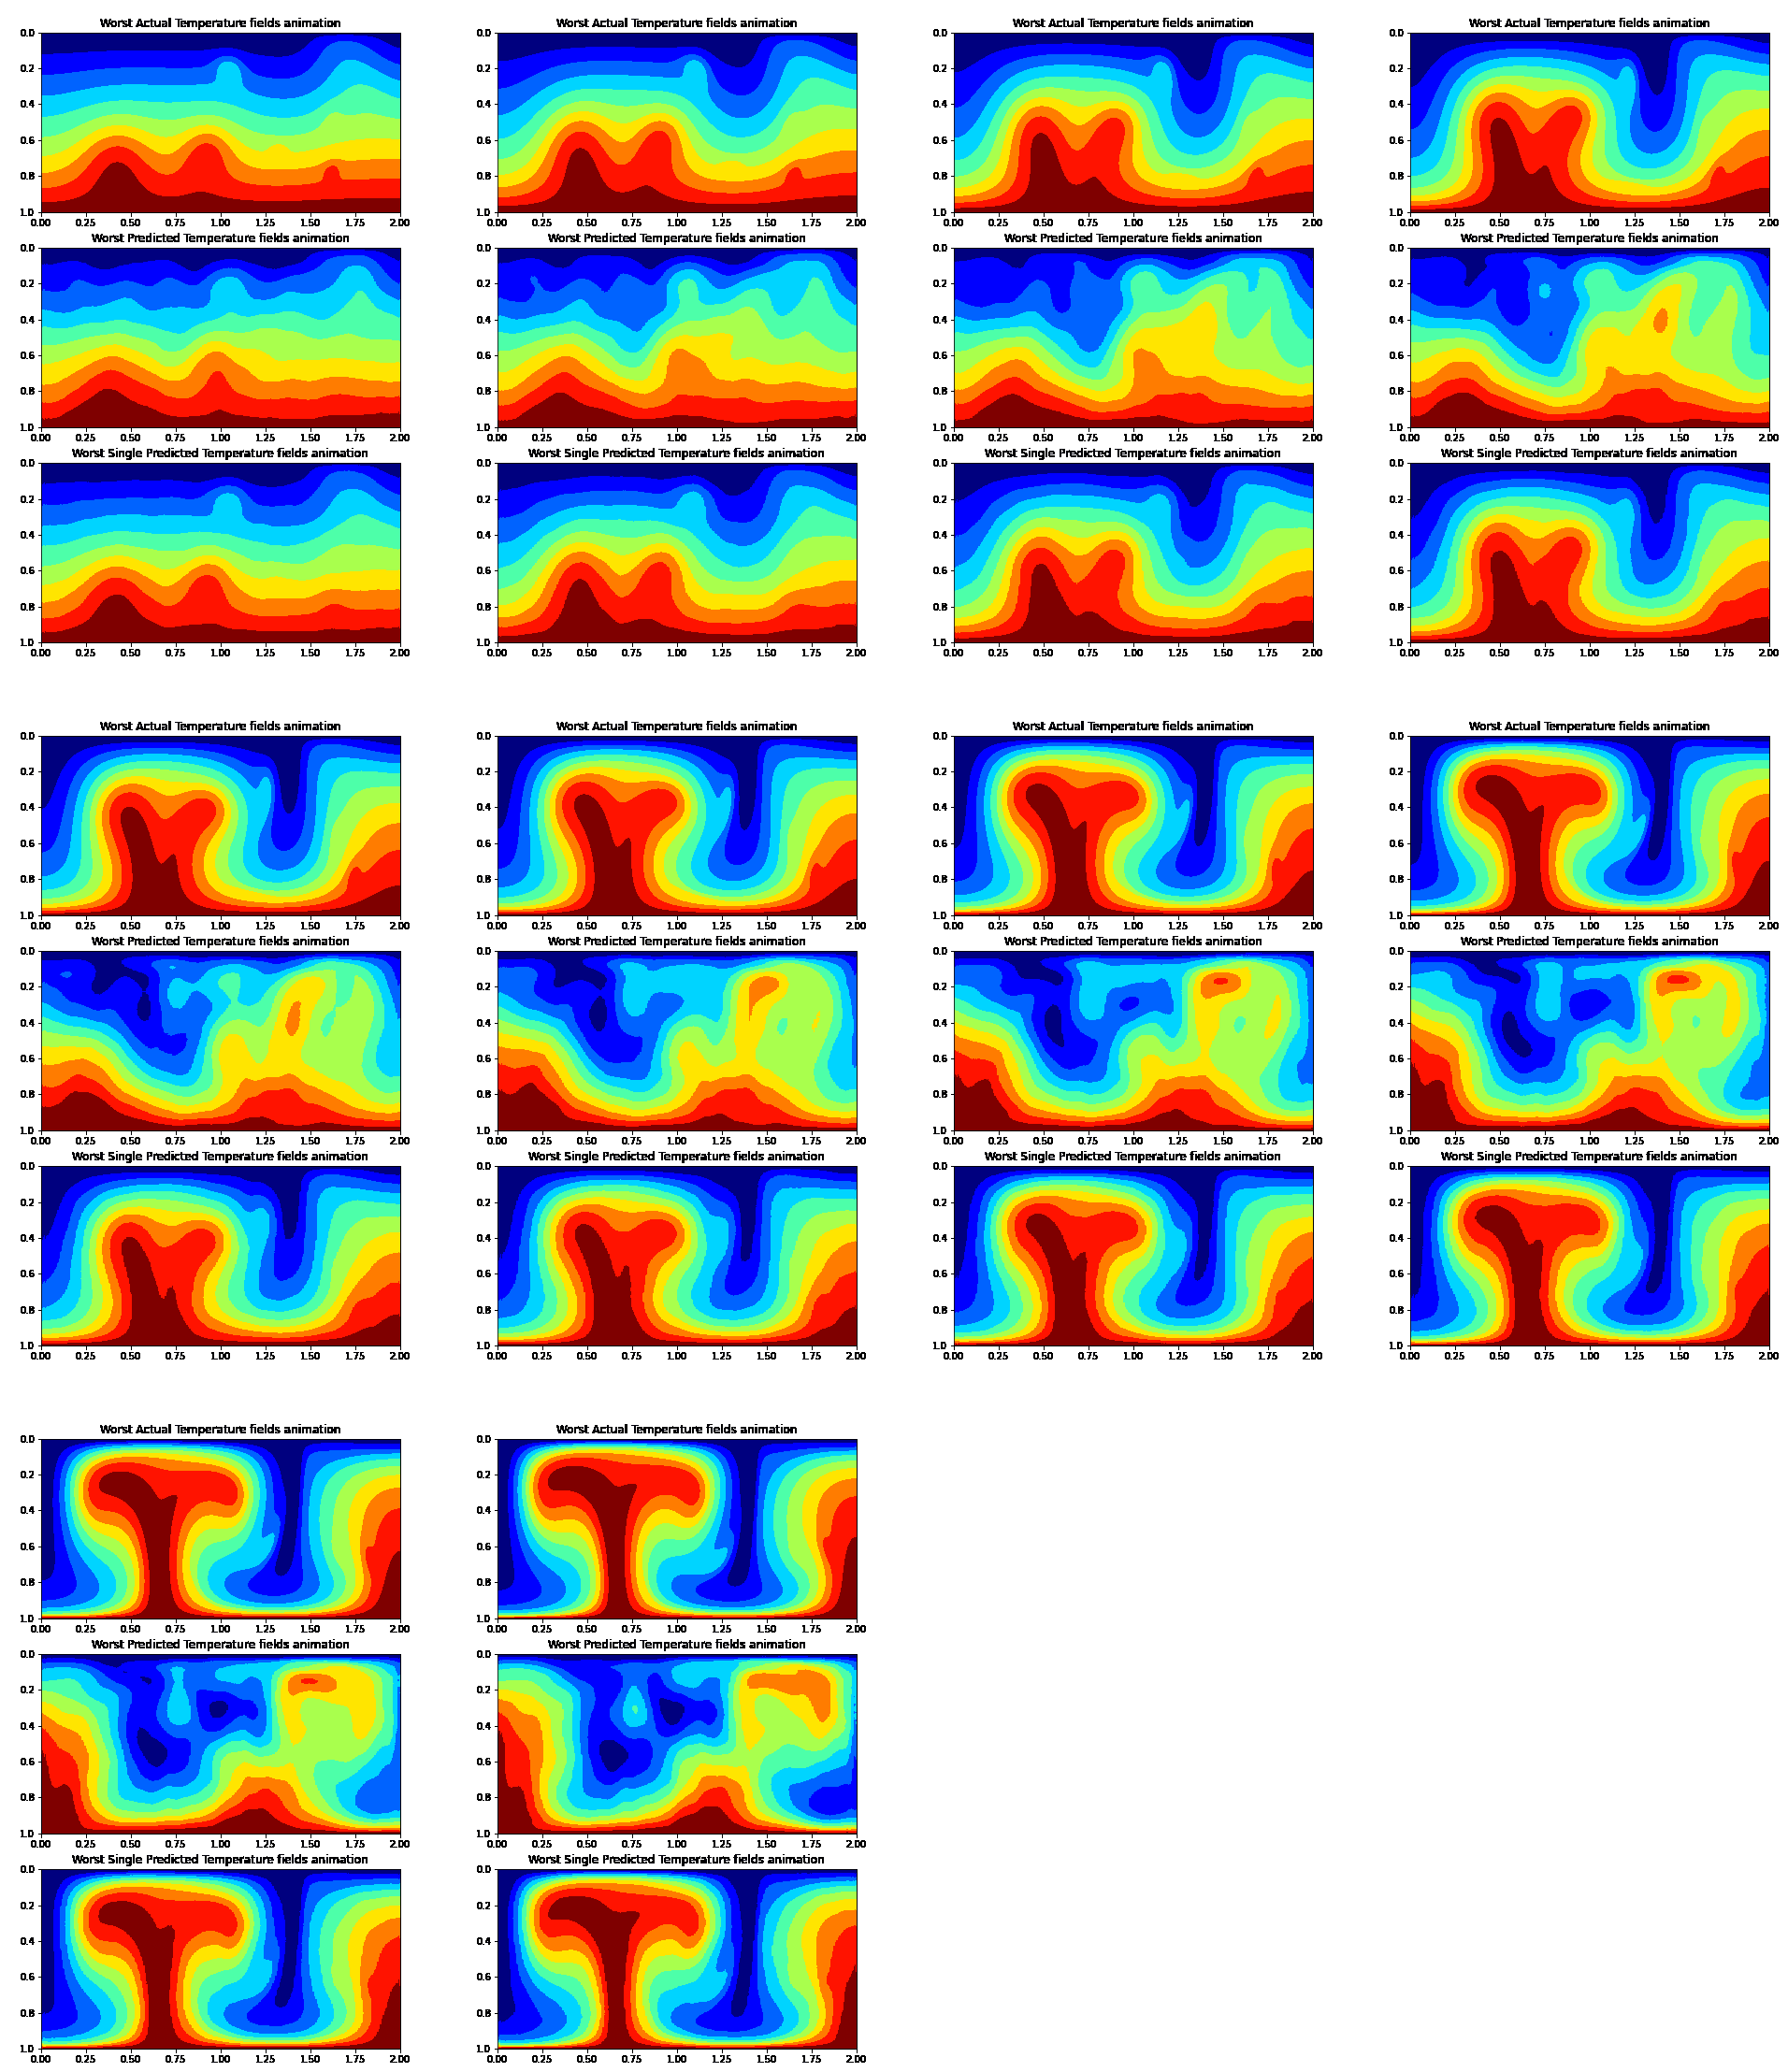
\includegraphics[scale=0.10]{figures/mantle_convection_images/larger_dataset/FNN_Worst_GIF_sheet.png}
    \label{figure:FNN_larger_worst_gif}
\end{figure}

POD result for the best case and worst case are shown by Figure \ref{figure:FNN_larger_best_POD} and Figure \ref{figure:FNN_larger_worst_POD}:

\begin{figure}[H]
    \caption{Best case POD of FNN trained with Larger Dataset.}
    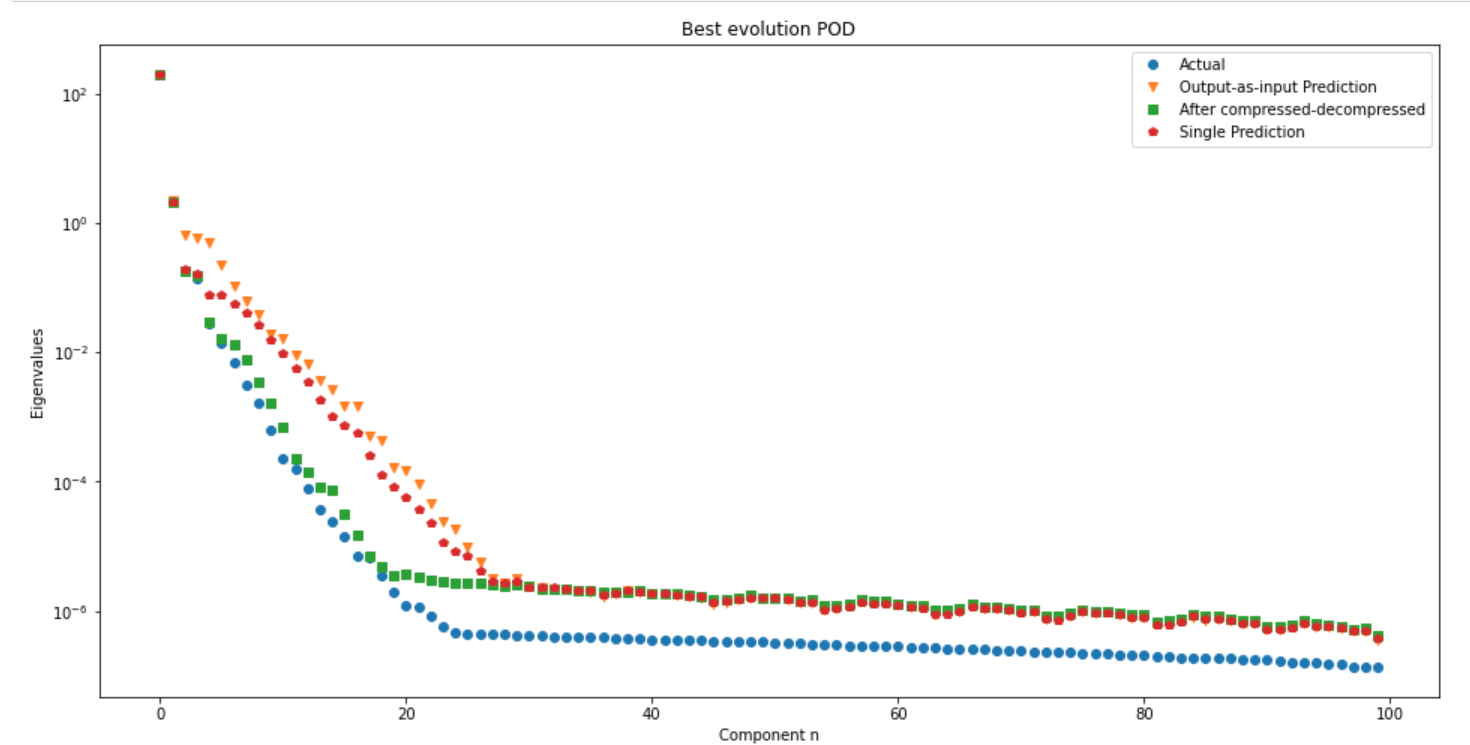
\includegraphics[scale=0.5]{figures/mantle_convection_images/larger_dataset/FNN_Best_POD.png}
    \label{figure:FNN_larger_best_POD}
\end{figure}

\begin{figure}[H]
    \caption{Worst case POD of FNN trained with Larger Dataset.}
    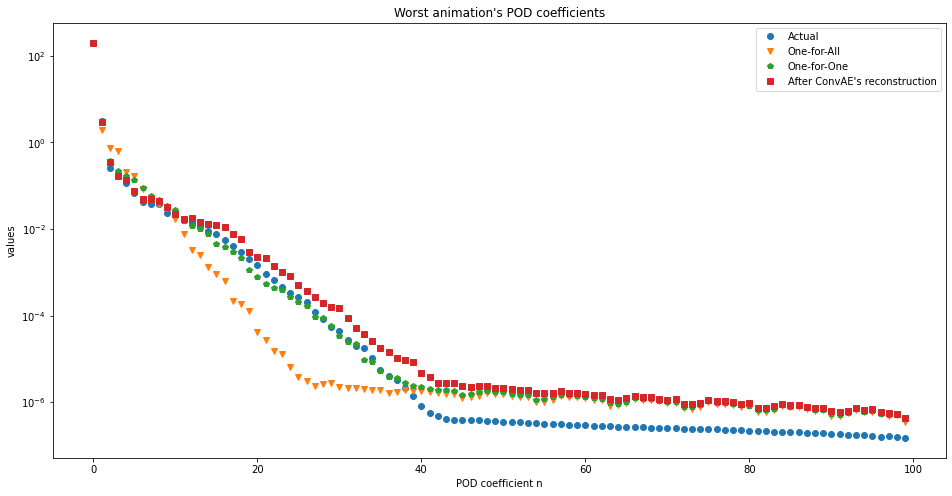
\includegraphics[scale=0.5]{figures/mantle_convection_images/larger_dataset/FNN_Worst_POD.png}
    \label{figure:FNN_larger_worst_POD}
\end{figure}

We can observe that the increasing size of the training data does not improve the quality of the animations when predicting the entire simulations using the first method. Also, apart from the information loss, the problem of the predicted GIFs moving too fast or too slow still exists.


\subsection{Long Short-Term Memory (LSTM) for Prediction}

The LSTM in this section also has the same structure and the same set of hyperparamters as the one trained with limited dataset, except that the total number of epochs are reduced from 200 to 100.

The results are presented in the following figures, including the training loss and validation loss from Figure \ref{figure:LSTM_larger_losses}, overall testing result from Figure \ref{figure:LSTM_larger_testing}, and the most/least accurate prediction in Figure \ref{figure:LSTM_larger_best} and Figure \ref{figure:LSTM_larger_worst}:

\begin{figure}[H]
    \caption{Training loss and Validation loss of LSTM trained with Larger Dataset.}
    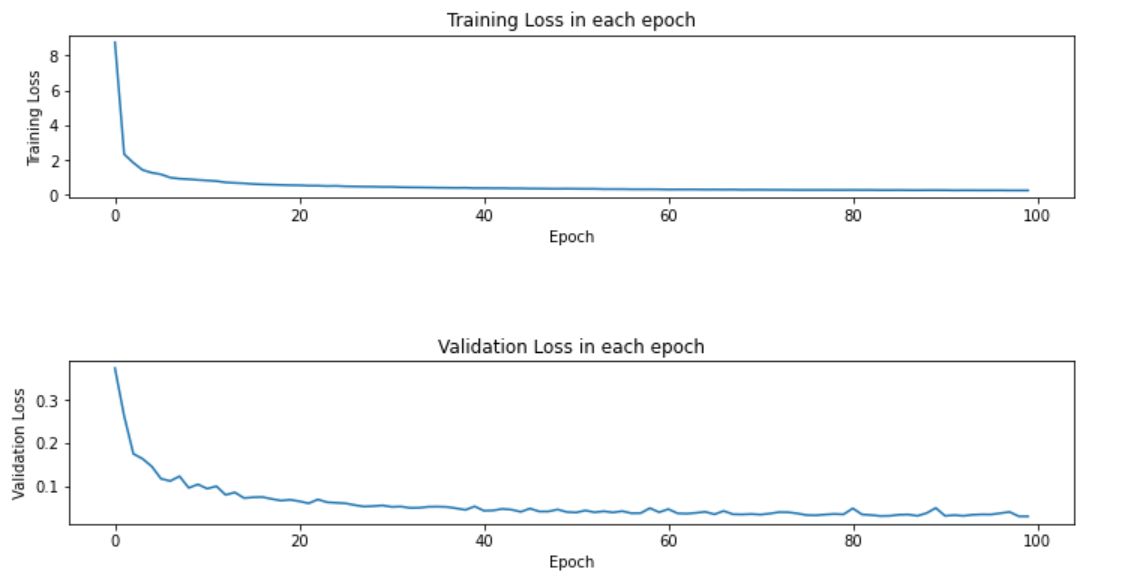
\includegraphics[scale=0.6]{figures/mantle_convection_images/larger_dataset/LSTM_trainingData.png}
    \label{figure:LSTM_larger_losses}
\end{figure}

\begin{figure}[H]
    \caption{Overall testing result of LSTM trained with Larger Dataset.}
    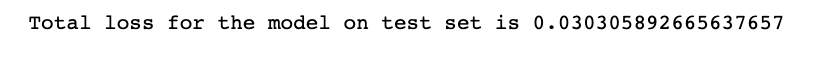
\includegraphics[scale=0.8]{figures/mantle_convection_images/larger_dataset/LSTM_OverallTesting.png}
    \label{figure:LSTM_larger_testing}
\end{figure}

\begin{figure}[H]
    \caption{Ground truth, ground truth after ConvAE's compression-decompression, and most accurate prediction of LSTM trained with Larger Dataset.}
    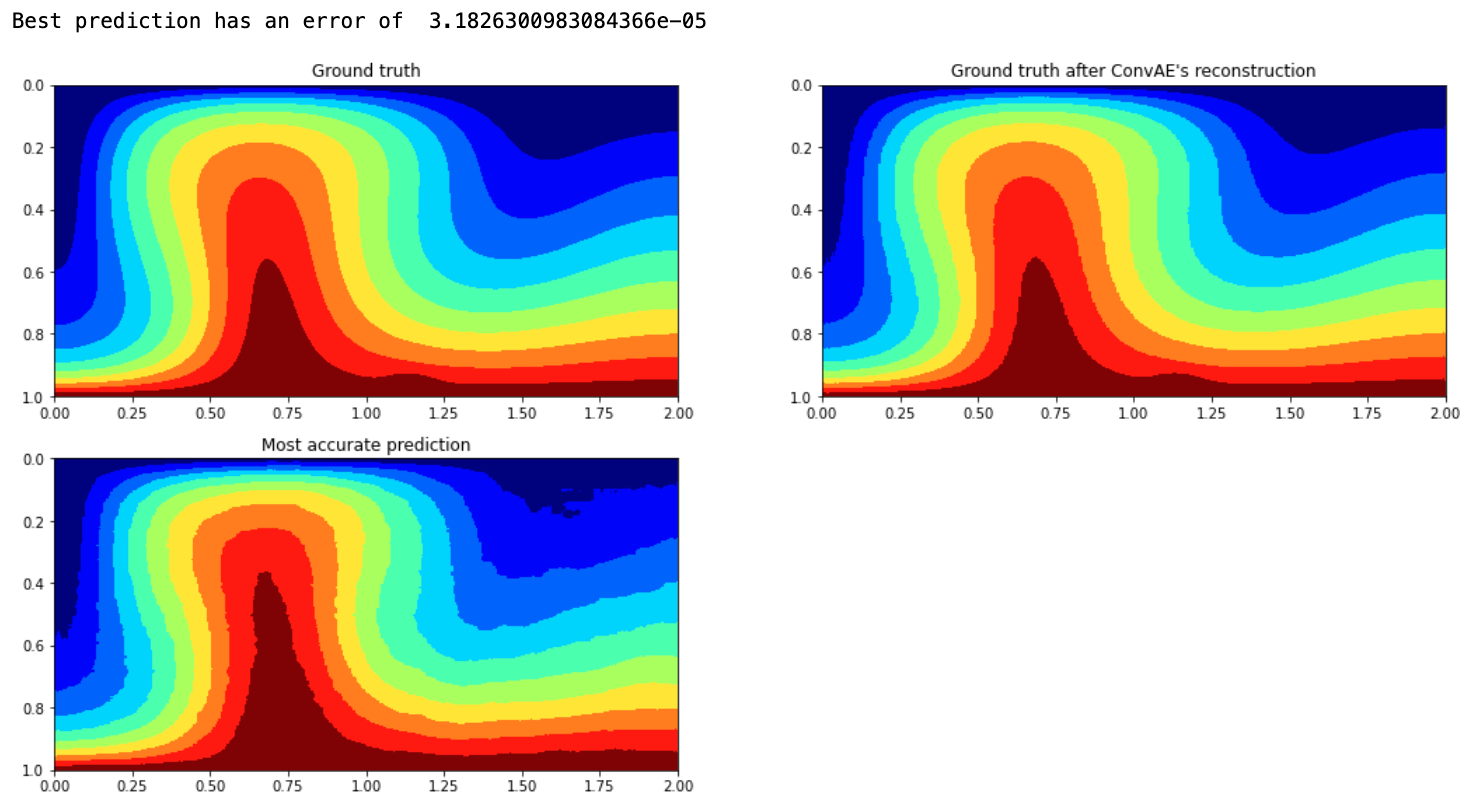
\includegraphics[scale=0.5]{figures/mantle_convection_images/larger_dataset/LSTM_Best.png}
    \label{figure:LSTM_larger_best}
\end{figure}

\begin{figure}[H]
    \caption{Ground truth, ground truth after ConvAE's compression-decompression, and least accurate prediction of LSTM trained with Larger Dataset.}
    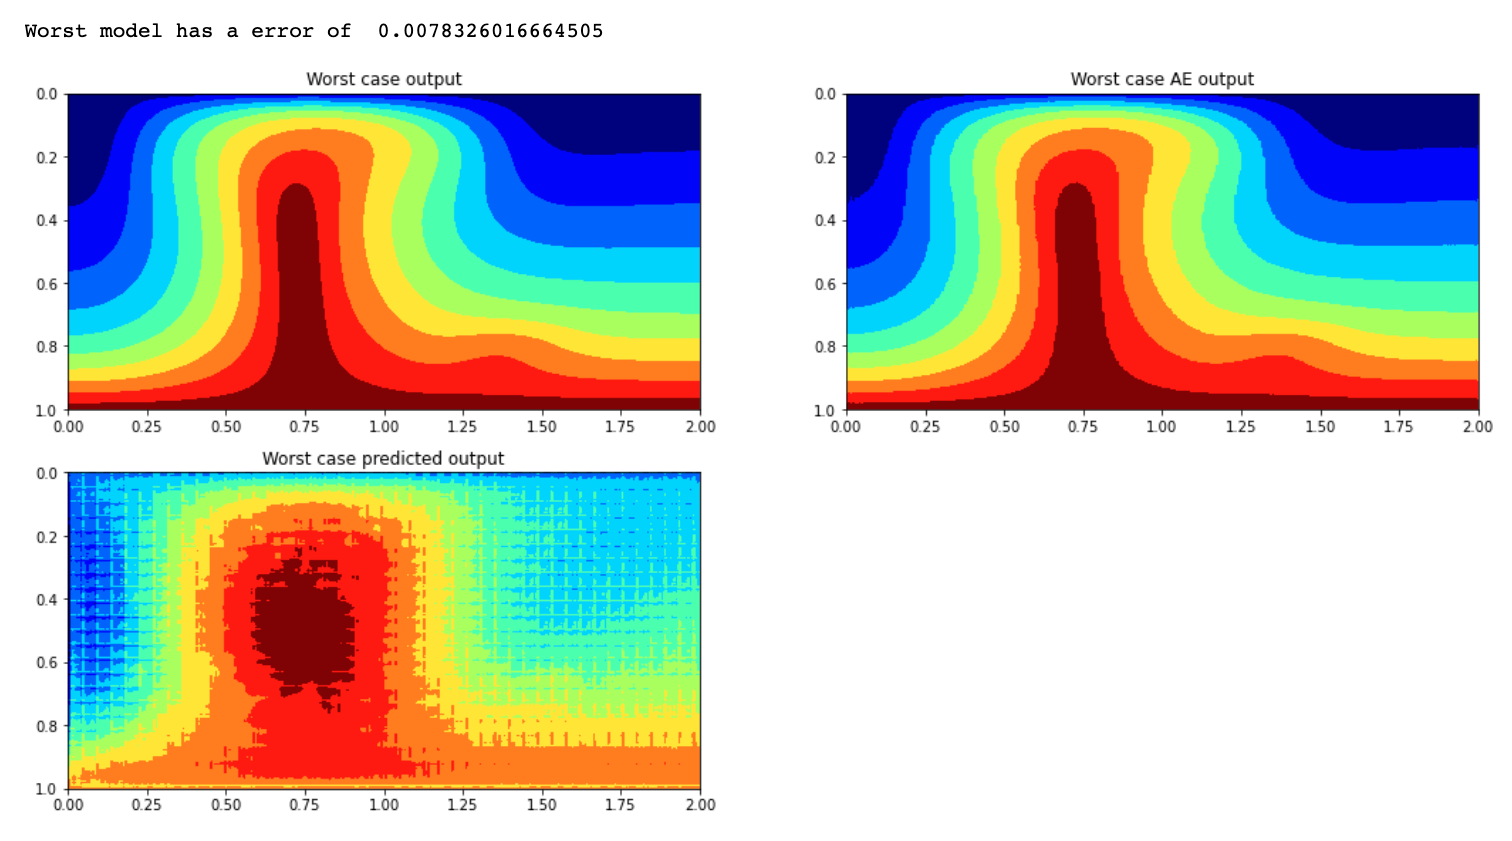
\includegraphics[scale=0.5]{figures/mantle_convection_images/larger_dataset/LSTM_Worst.png}
    \label{figure:LSTM_larger_worst}
\end{figure}


From the above figures, we can see that the loss of the best case and the worst case for this LSTM are in the same level as the one trained with limited dataset given 10 times of the training data, which means that the low accuracy of LSTM is not caused by some potential underfitting problem as discussed in the last section.

For better visualisation as well, two animations representing the best case and the worst case when predicting the rest of the simulation using the first 50 temperature fields are generated.

Figure \ref{figure:LSTM_larger_best_gif} and Figure \ref{figure:LSTM_larger_worst_gif} show 20\% of the two sprite sheets converted from the original GIF animations (Every 5th frame):

\begin{figure}[H]
    \centering
    \caption{Best case animation sheet of LSTM trained with Larger Dataset (Link to this GIF: \url{https://drive.google.com/file/d/1UFYSPVLT1wRsKM5GAdCz0JQLZF8OKNUc/view?usp=sharing})}
    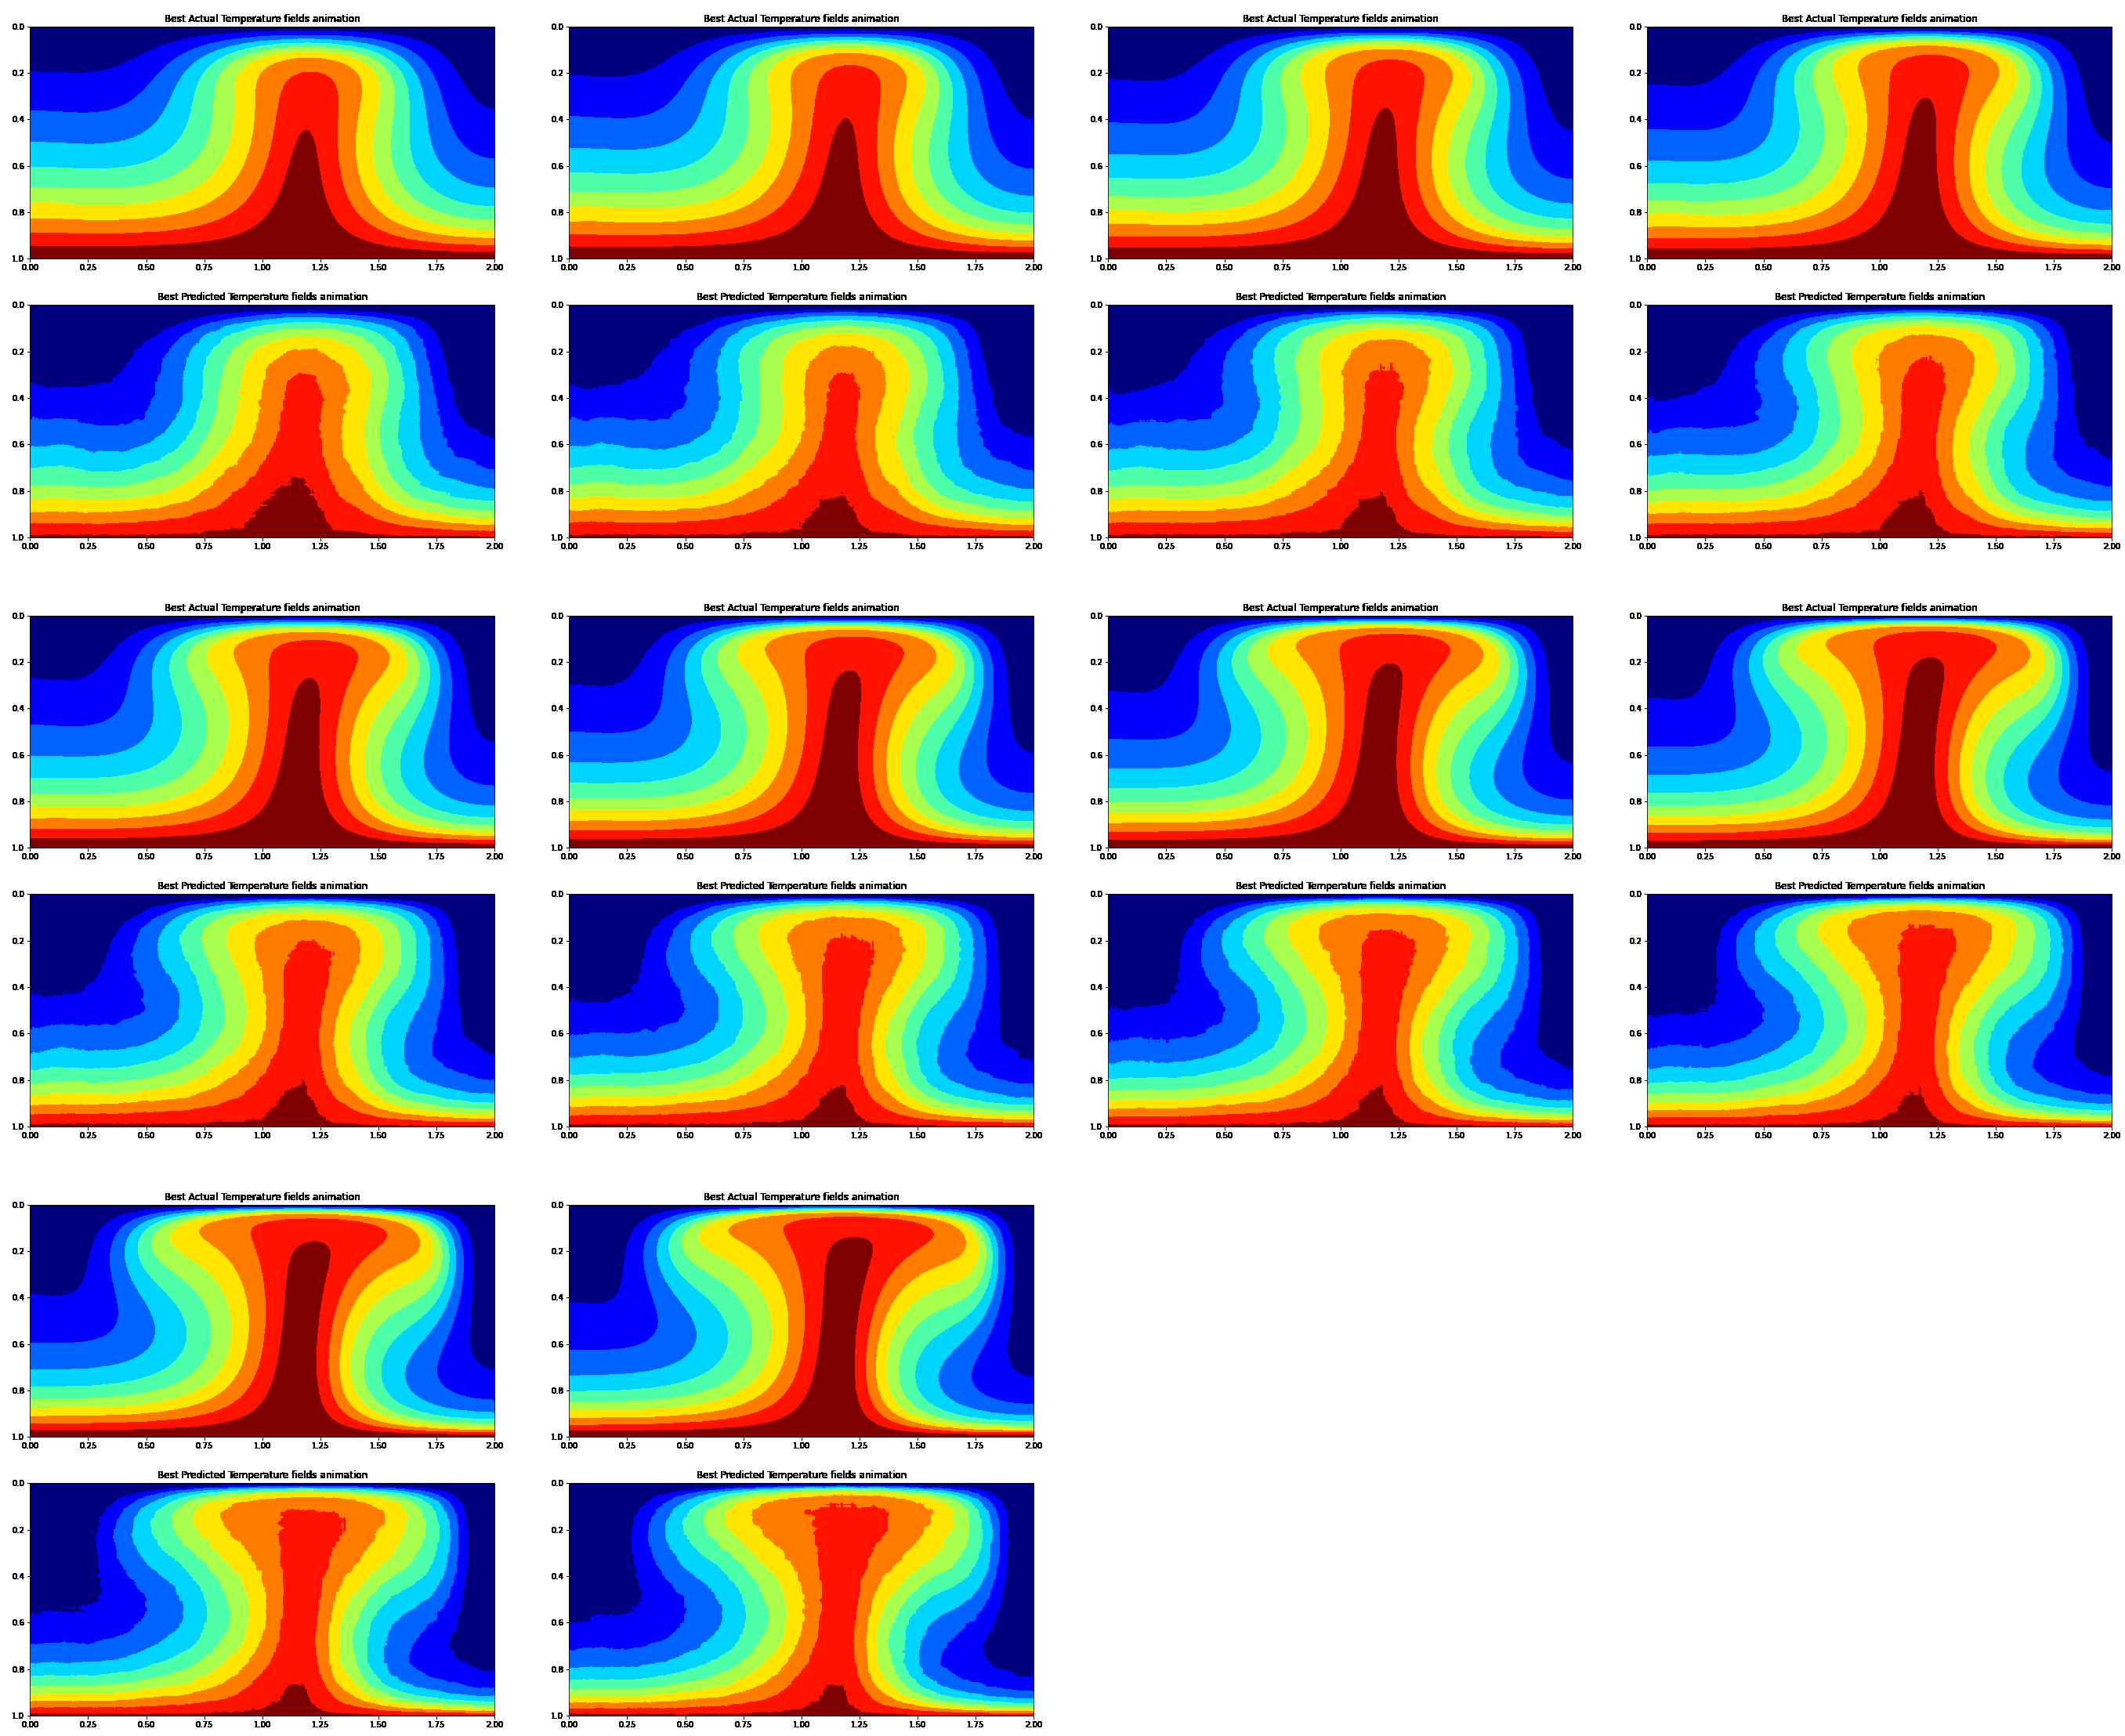
\includegraphics[scale=0.10]{figures/mantle_convection_images/larger_dataset/LSTM_Best_GIF_sheet.png}
    \label{figure:LSTM_larger_best_gif}
\end{figure}



\begin{figure}[H]
    \centering
    \caption{Worst case animation sheet of LSTM trained with Larger Dataset (Link to this GIF: 
    \url{https://drive.google.com/file/d/1SbzjPwwe7FCu7JCJru8UYHOu9j6uVfZd/view?usp=sharing})}
    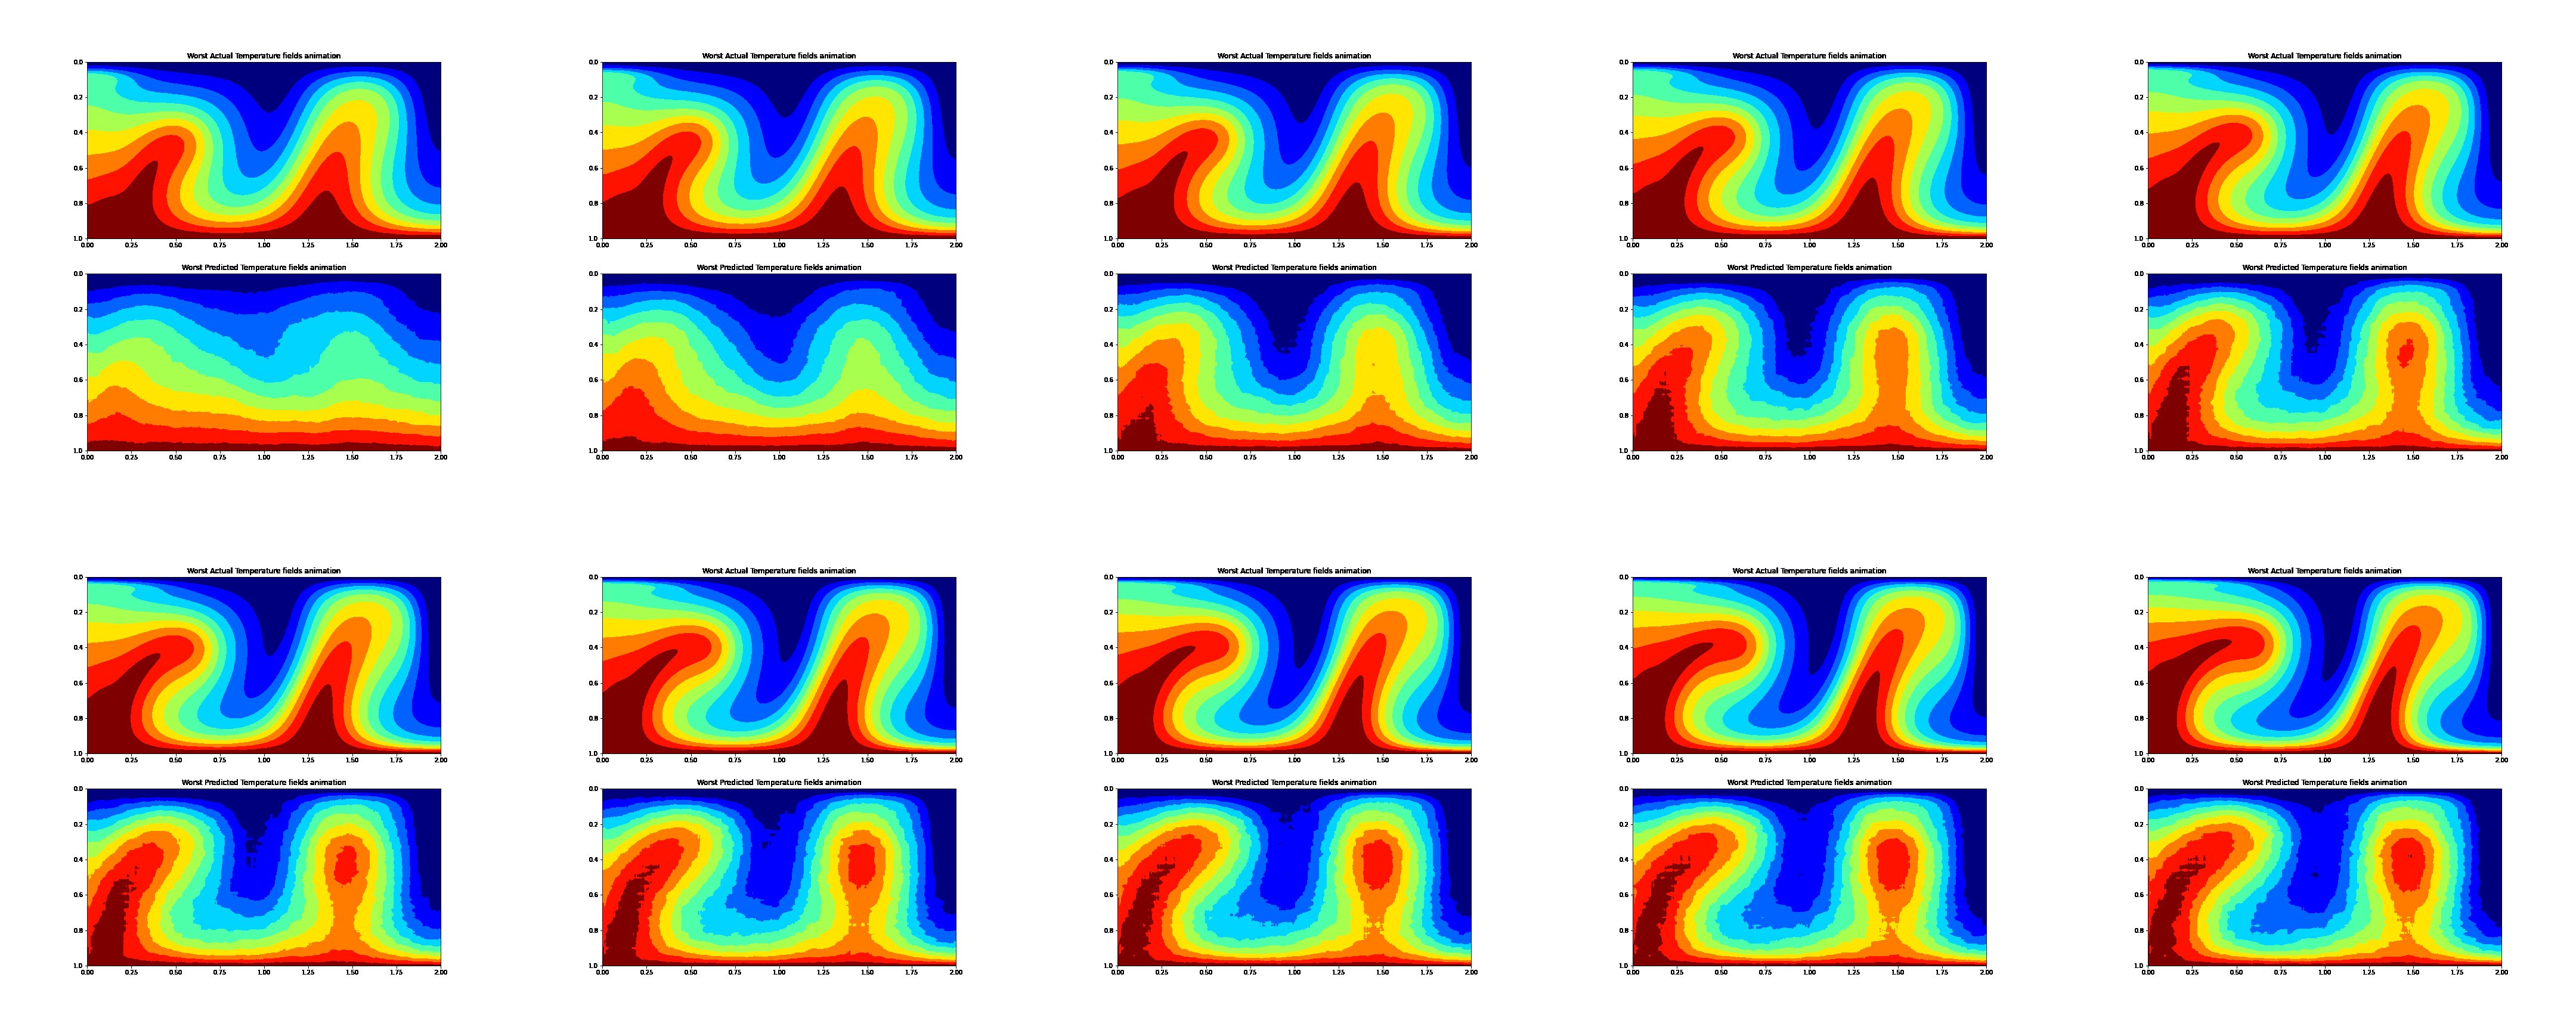
\includegraphics[scale=0.10]{figures/mantle_convection_images/larger_dataset/LSTM_Worst_GIF_sheet.png}
    \label{figure:LSTM_larger_worst_gif}
\end{figure}

POD result for the best case and worst case are shown in Figure \ref{figure:LSTM_larger_best_POD} and Figure \ref{figure:LSTM_larger_worst_POD}:

\begin{figure}[H]
    \caption{Best case POD of LSTM trained with Larger Dataset.}
    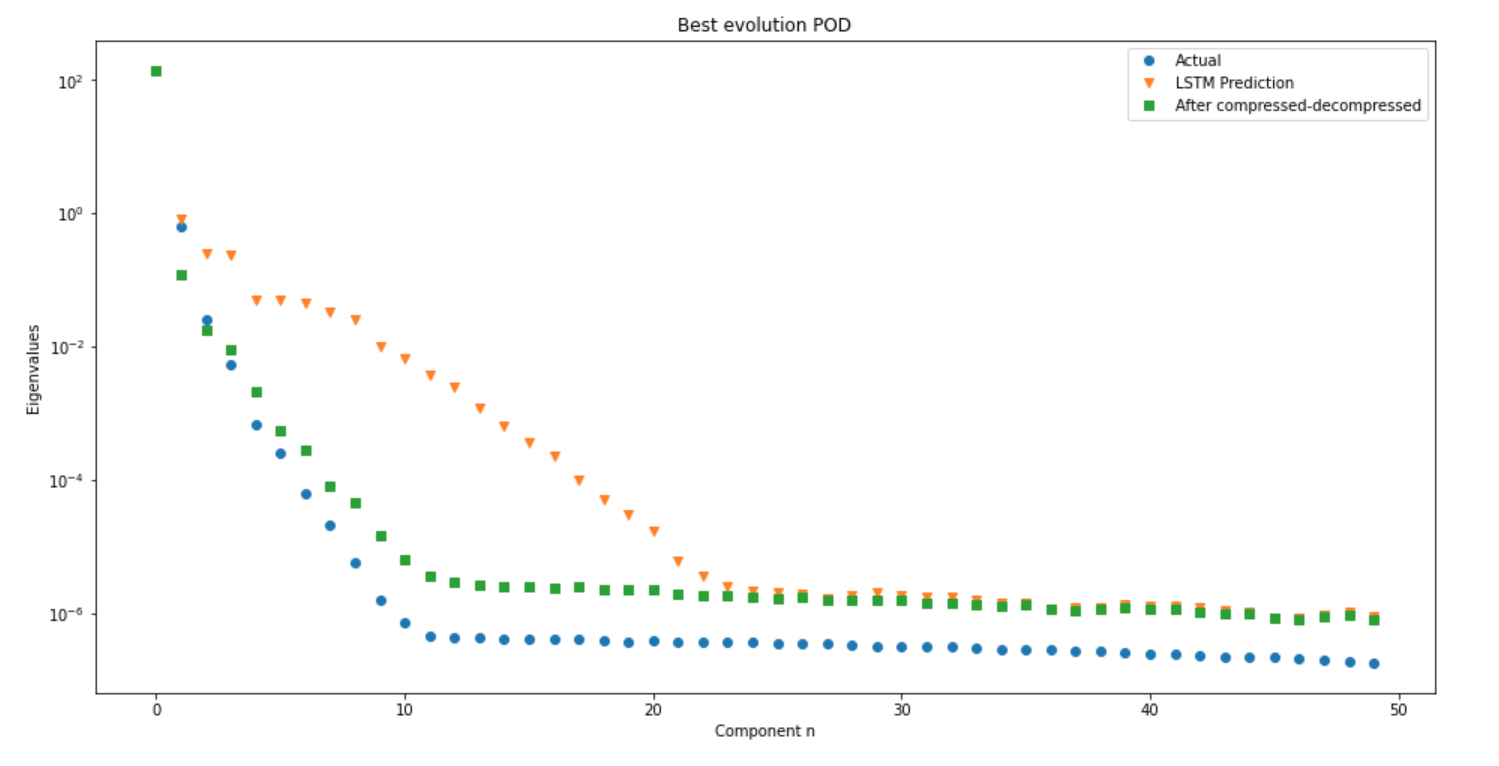
\includegraphics[scale=0.5]{figures/mantle_convection_images/larger_dataset/LSTM_Best_POD.png}
    \label{figure:LSTM_larger_best_POD}
\end{figure}

\begin{figure}[H]
    \caption{Worst case POD of LSTM trained with Larger Dataset.}
    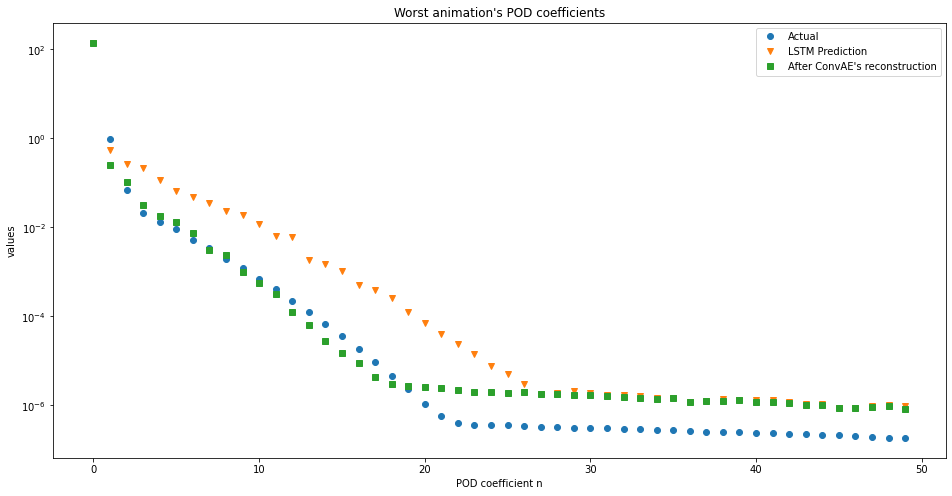
\includegraphics[scale=0.5]{figures/mantle_convection_images/larger_dataset/LSTM_Worst_POD.png}
    \label{figure:LSTM_larger_worst_POD}
\end{figure}

From the animations and the POD results, we can now confirmed that LSTM is able to capture most of characteristics of the simulations even in its worst case and the simulations predicted using LSTM are less accurate compared with those predicted using FNN.


\section{Mantle Convection Simulation on Interpolated Dataset}

To confirm if the problem of the predicted GIFs moving too fast or too slow is caused by the varying distance between time steps, an interpolated dataset is created using the larger dataset in the last section.

The interpolation process is done for each of the simulation separately by generating a sequence of temperature fields with equal distance between their consecutive time steps. The resulting sequence of time steps for every interpolated simulations are the same by giving a start time step (close to the minimum time step), an end time step (close to the maximum time step) and the number of samples (=100) to generate a new evenly spaced time step sequence to interpolate with. In order to retrieve the temperature field at the target time step, the temperature fields at two nearest time steps are searched for and the target temperature field is generated by interpolating between these two temperature fields.

After the interpolation process, we are able to get an interpolation dataset where every simulation has the same time steps.

The interpolated dataset are also randomly divided in the same way as the limited dataset for each of the three ML architectures in the following subsections.


\subsection{Compression of temperature fields}

The ConvAE used for compressing the temperature fields in this section has the same structure and the same set of hyperparameters as the one trained with the original larger dataset.

In the following figures, some detailed test results from this ConvAE trained with interpolated dataset are presented, including the training loss and validation loss from Figure \ref{figure:ConvAE_interpolated_losses}, overall testing result from Figure \ref{figure:ConvAE_interpolated_testing}, and the most/least accurate prediction in Figure \ref{figure:ConvAE_interpolated_best_worst}:


\begin{figure}[H]
    \caption{Training loss and Validation loss of ConvAE trained with Interpolated Dataset.}
    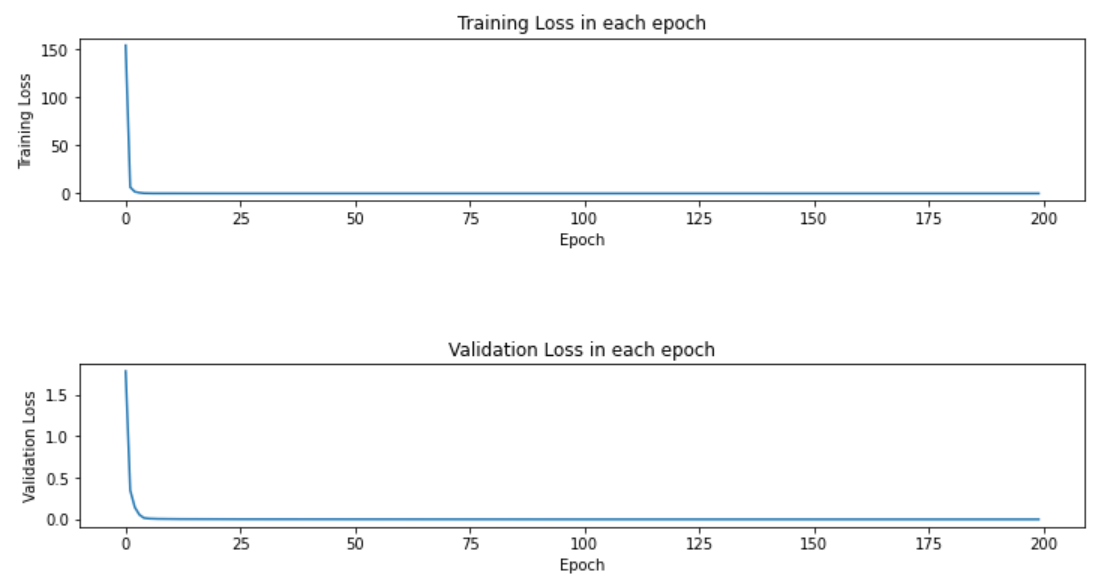
\includegraphics[scale=0.6]{figures/mantle_convection_images/larger_dataset_interpolated/ConvAE_trainingData.png}
    \label{figure:ConvAE_interpolated_losses}
\end{figure}

\begin{figure}[H]
    \caption{Overall testing result of ConvAE trained with Interpolated Dataset.}
    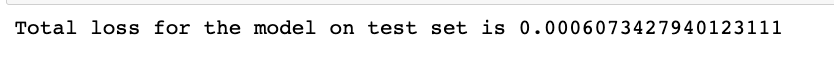
\includegraphics[scale=0.8]{figures/mantle_convection_images/larger_dataset_interpolated/ConvAE_OverallTesting.png}
    \label{figure:ConvAE_interpolated_testing}
\end{figure}

\begin{figure}[H]
\centering
\begin{subfigure}{0.45\textwidth}
    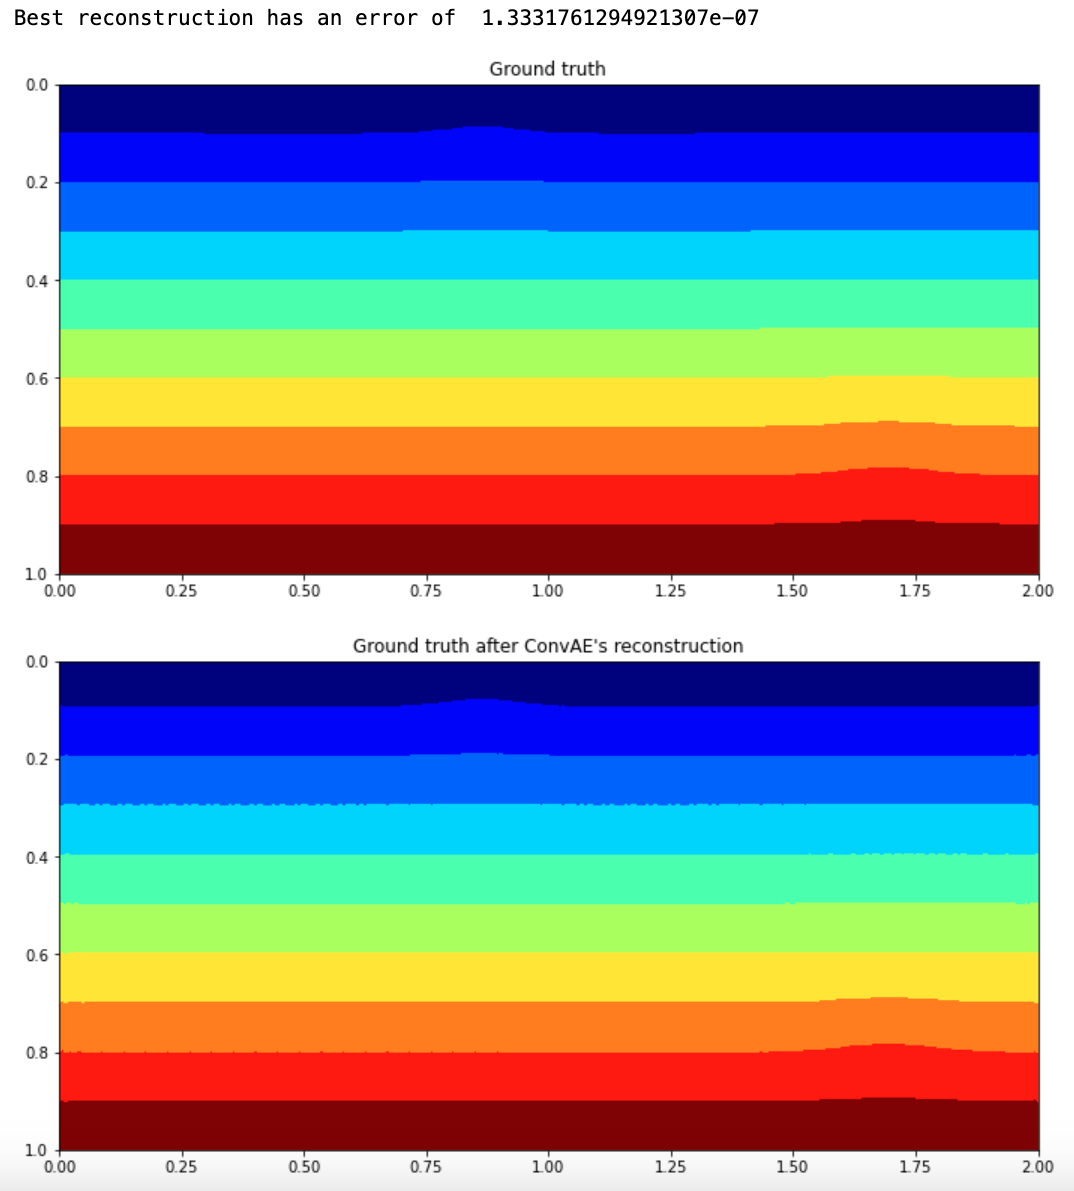
\includegraphics[width=\textwidth]{figures/mantle_convection_images/larger_dataset_interpolated/ConvAE_Best.png}
    \caption{Most accurate reconstruction of ConvAE trained with Interpolated Dataset.}
\end{subfigure}
\hfill
\begin{subfigure}{0.45\textwidth}
    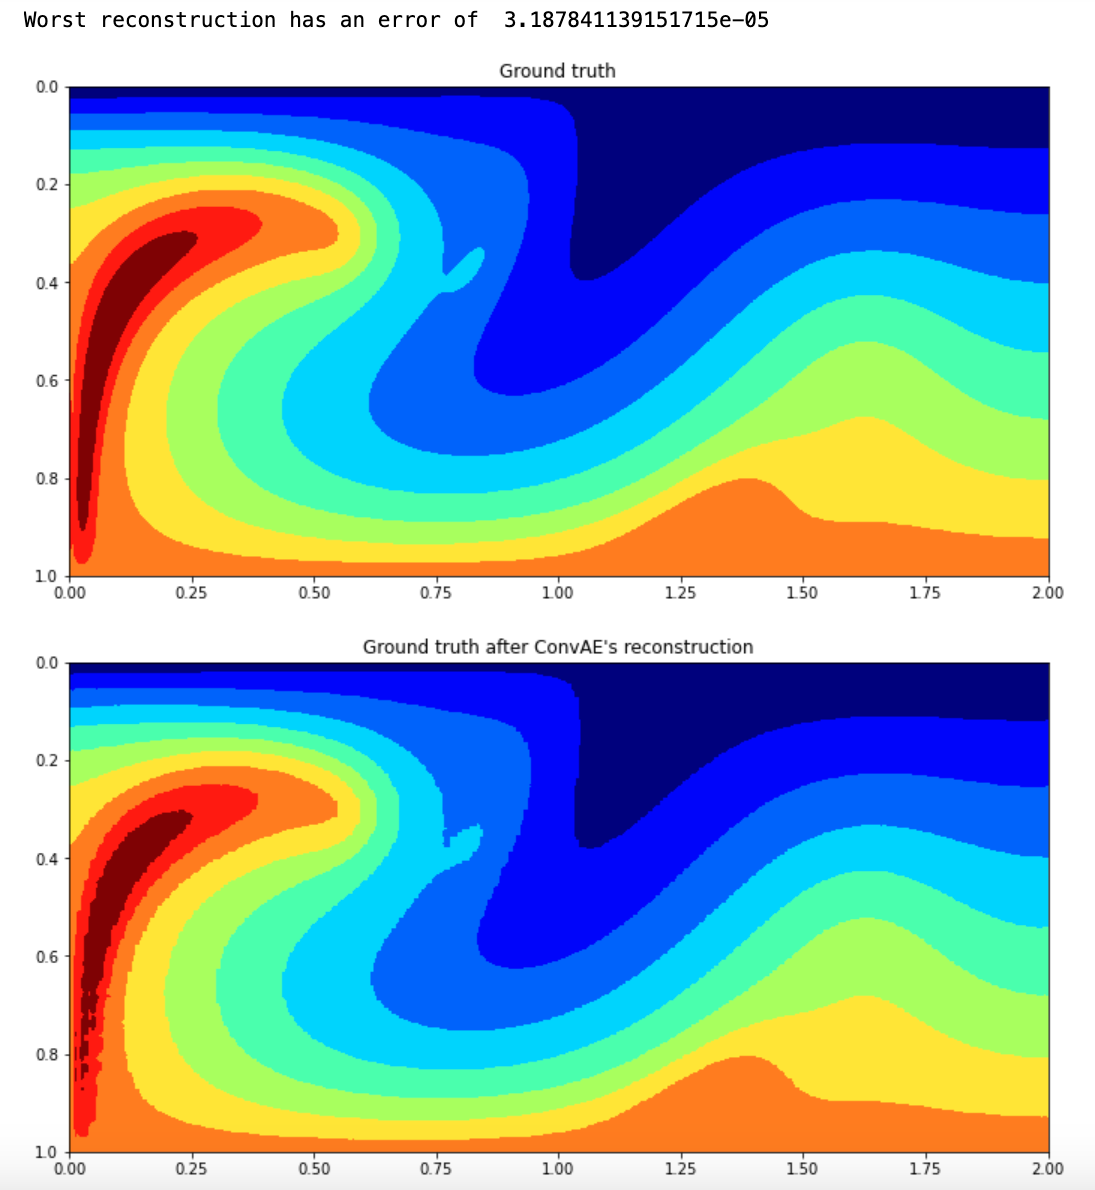
\includegraphics[width=\textwidth]{figures/mantle_convection_images/larger_dataset_interpolated/ConvAE_Worst.png}
    \caption{Least accurate reconstruction of ConvAE trained with Interpolated Dataset.}
\end{subfigure}
\caption{Best case and worst case using ConvAE.}
\label{figure:ConvAE_interpolated_best_worst}
\end{figure}

We can observe that the performance of this ConvAE is better than the one trained with the original larger dataset since it has a total loss that is 3 times lower than the one in the last section (0.0005 to 0.0016). This could imply that the interpolated data make the training process of ConvAE easier given the same size of data. 


\subsection{Fully Connected Neural Network for Prediction}

The FNN in this section also has the same structure and the same set of hyperparameters as the one trained with the original larger dataset.

The results are presented in the following figures, including the training loss and validation loss from Figure \ref{figure:FNN_interpolated_losses}, overall testing result from Figure \ref{figure:FNN_interpolated_testing}, and the most/least accurate prediction in Figure \ref{figure:FNN_interpolated_best} and Figure \ref{figure:FNN_interpolated_worst}:

\begin{figure}[H]
    \caption{Training loss and Validation loss of FNN trained with Interpolated Dataset.}
    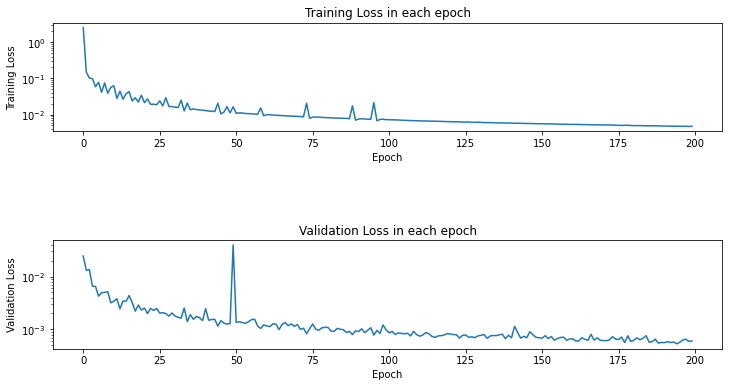
\includegraphics[scale=0.6]{figures/mantle_convection_images/larger_dataset_interpolated/FNN_trainingData.png}
    \label{figure:FNN_interpolated_losses}
\end{figure}

\begin{figure}[H]
    \caption{Overall testing result of FNN trained with Interpolated Dataset.}
    \includegraphics[scale=0.8]{figures/mantle_convection_images/larger_dataset_interpolated/FNN_OverallTesting.png}
    \label{figure:FNN_interpolated_testing}
\end{figure}

\begin{figure}[H]
    \caption{Ground truth, ground truth after ConvAE's compression-decompression, and most accurate prediction of FNN trained with Interpolated Dataset.}
    \includegraphics[scale=0.5]{figures/mantle_convection_images/larger_dataset_interpolated/FNN_Best.png}
    \label{figure:FNN_interpolated_best}
\end{figure}

\begin{figure}[H]
    \caption{Ground truth, ground truth after ConvAE's compression-decompression, and least accurate prediction of FNN trained with Interpolated Dataset.}
    \includegraphics[scale=0.5]{figures/mantle_convection_images/larger_dataset_interpolated/FNN_Worst.png}
    \label{figure:FNN_interpolated_worst}
\end{figure}

The above result of this FNN are better than the one trained with the original larger dataset since the loss values are 2 times lower than the one in the last section (0.0005 to 0.0011), which could be partially due to the better performance of the ConvAE.

Again, two animations representing the best case and the worst case when predicting the entire simulation using "One-for-All" method (use $T1$ from dataset $\rightarrow$ get predicted $T2$ $\rightarrow$ use predicted $T2$ $\rightarrow$ get predicted $T3$ $\rightarrow$ ...) are generated.

Figure \ref{figure:FNN_interpolated_best_gif} and Figure \ref{figure:FNN_interpolated_worst_gif} show 10\% of the sprite sheets converted from the original GIF animations (Every 10th frame):

\begin{figure}[H]
    \centering
    \caption{Best case animation sheet of FNN trained with Interpolated Dataset (Link to this GIF: \url{https://drive.google.com/file/d/10znEe7q_A0rndmuivlbWBH8sZEH6Gv3p/view?usp=sharing})}
    \includegraphics[scale=0.10]{figures/mantle_convection_images/larger_dataset_interpolated/FNN_Best_GIF_sheet.png}
    \label{figure:FNN_interpolated_best_gif}
\end{figure}

\begin{figure}[H]
    \centering
    \caption{Worst case animation sheet of FNN trained with Interpolated Dataset (Link to this GIF: 
    \url{https://drive.google.com/file/d/1vIXrWn6emumszEy3VDArqdenj3FQeVVa/view?usp=sharing})}
    \includegraphics[scale=0.10]{figures/mantle_convection_images/larger_dataset_interpolated/FNN_Worst_GIF_sheet.png}
    \label{figure:FNN_interpolated_worst_gif}
\end{figure}

Figure \ref{figure:FNN_interpolated_best_POD} and Figure \ref{figure:FNN_interpolated_worst_POD} show the POD result in the best case and the worst case:

\begin{figure}[H]
    \caption{Best case POD of FNN trained with Interpolated Dataset.}
    \includegraphics[scale=0.5]{figures/mantle_convection_images/larger_dataset_interpolated/FNN_Best_POD.png}
    \label{figure:FNN_interpolated_best_POD}
\end{figure}

\begin{figure}[H]
    \caption{Worst case POD of FNN trained with Interpolated Dataset.}
    \includegraphics[scale=0.5]{figures/mantle_convection_images/larger_dataset_interpolated/FNN_Worst_POD.png}
    \label{figure:FNN_interpolated_worst_POD}
\end{figure}

We can observe that the problem of predicted GIFs moving faster or slower than the actual simulations is now gone. Also, the POD result in the worst case is now closer than the one in the original simulations. This confirmed that the varying time steps are the cause of the inconsistent GIF speed and by fixing this issue using an interpolated dataset, the performance of the FNN is able to be improved.


\subsection{Long Short-Term Memory (LSTM) for Prediction}

The LSTM in this section also has the same structure and the same set of hyperparameters as the one trained with the original larger dataset.

The results are presented in the following figures, including the training loss and validation loss from Figure \ref{figure:LSTM_interpolated_losses}, overall testing result from Figure \ref{figure:LSTM_interpolated_testing}, and the most/least accurate prediction in Figure \ref{figure:LSTM_interpolated_best} and Figure \ref{figure:LSTM_interpolated_worst}:


\begin{figure}[H]
    \caption{Training loss and Validation loss of LSTM trained with Interpolated Dataset.}
    \includegraphics[scale=0.6]{figures/mantle_convection_images/larger_dataset_interpolated/LSTM_trainingData.png}
    \label{figure:LSTM_interpolated_losses}
\end{figure}

\begin{figure}[H]
    \caption{Overall testing result of LSTM trained with Interpolated Dataset.}
    \includegraphics[scale=0.8]{figures/mantle_convection_images/larger_dataset_interpolated/LSTM_OverallTesting.png}
    \label{figure:LSTM_interpolated_testing}
\end{figure}

\begin{figure}[H]
    \caption{Ground truth, ground truth after ConvAE's compression-decompression, and most accurate prediction of LSTM trained with Interpolated Dataset.}
    \includegraphics[scale=0.5]{figures/mantle_convection_images/larger_dataset_interpolated/LSTM_Best.png}
    \label{figure:LSTM_interpolated_best}
\end{figure}

\begin{figure}[H]
    \caption{Ground truth, ground truth after ConvAE's compression-decompression, and least accurate prediction of LSTM trained with Interpolated Dataset.}
    \includegraphics[scale=0.5]{figures/mantle_convection_images/larger_dataset_interpolated/LSTM_Worst.png}
    \label{figure:LSTM_interpolated_worst}
\end{figure}

From the above figures, we can see that the loss of the best case and the average loss of this LSTM is now less than the one trained with the original larger dataset, which means that the interpolation process improves the accuracy when using LSTM as well.

Again, two animations representing the best case and the worst case when predicting the rest of the simulation using the first 50 temperature fields are generated.

Figure \ref{figure:LSTM_interpolated_best_gif} and Figure \ref{figure:LSTM_interpolated_worst_gif} show 20\% of the two sprite sheets converted from the original GIF animations (Every 5th frame):

\begin{figure}[H]
    \centering
    \caption{Best case animation sheet of LSTM trained with Interpolated Dataset (Link to this GIF: \url{https://drive.google.com/file/d/1fNkJVHw3v8WzVz0IKcPfI9rwmwhYygWS/view?usp=sharing})}
    \includegraphics[scale=0.10]{figures/mantle_convection_images/larger_dataset_interpolated/LSTM_Best_GIF_sheet.png}
     \label{figure:LSTM_interpolated_best_gif}
\end{figure}

\begin{figure}[H]
    \centering
    \caption{Worst case animation sheet of LSTM trained with Interpolated Dataset (Link to this GIF: 
    \url{https://drive.google.com/file/d/1JbhX4Zznv9YXHZi8IG811495_-YTOq9l/view?usp=sharing})}
    \includegraphics[scale=0.10]{figures/mantle_convection_images/larger_dataset_interpolated/LSTM_Worst_GIF_sheet.png}
    \label{figure:LSTM_interpolated_worst_gif}
\end{figure}

Figure \ref{figure:LSTM_interpolated_best_POD} and Figure \ref{figure:LSTM_interpolated_worst_POD} show the POD result in best case and the worst case:

\begin{figure}[H]
    \caption{Best case POD of LSTM trained with Interpolated Dataset.}
    \includegraphics[scale=0.5]{figures/mantle_convection_images/larger_dataset_interpolated/LSTM_Best_POD.png}
    \label{figure:LSTM_interpolated_best_POD}
\end{figure}

\begin{figure}[H]
    \caption{Worst case POD of LSTM trained with Interpolated Dataset.}
    \includegraphics[scale=0.5]{figures/mantle_convection_images/larger_dataset_interpolated/LSTM_Worst_POD.png}
    \label{figure:LSTM_interpolated_worst_POD}
\end{figure}


We can observe that the problem of predicted GIFs moving faster or slower than the actual simulations is gone, which is consistent with our conclusion in the last subsection.




\section{Further testings on Fully Connected Neural Network}

To determine experimentally for how many time steps we can use the trained FNN during a set of S consecutive time steps (e.g., S=2, S=4, or S=8, and then "correct" the time series with the truth coming from the simulator) without loosing track of the transient dynamics (that is, how large can S be without significantly affecting accuracy), further testings extending the two methods in the FNN section are done over the entire interpolated dataset using the trained FNN.

To compare against different values of S, POD are applied for each of the generated temperature field sequence to compare the difference of the eigenvalues between the predicted simulations and actual simulations. The data loss for each simulation are computed as well. The result for S = 1, 2, 4, 8, 16, 99 are shown as below (where S=1 is essentially the first method in the FNN section and S=99 is the second method), including the data loss shown by Figure \ref{figure:further_loss}, POD difference shown by Figure \ref{figure:further_POD} and Relative POD difference shown by Figure \ref{figure:further_relative_POD}:

\begin{figure}[H]
    \caption{Data Loss for S consecutive time steps.}
    \includegraphics[scale=0.7]{figures/mantle_convection_images/further_testings/Data_Loss_table.png}
    \label{figure:further_loss}
\end{figure}

\begin{figure}[H]
    \caption{POD difference for S consecutive time steps.}
    \includegraphics[scale=0.7]{figures/mantle_convection_images/further_testings/POD_table.png}
    \label{figure:further_POD}
\end{figure}

\begin{figure}[H]
    \caption{Relative POD difference for S consecutive time steps.}
    \includegraphics[scale=0.7]{figures/mantle_convection_images/further_testings/Relative_POD_table.png}
    \label{figure:further_relative_POD}
\end{figure}

To further evaluate the performance, a series of box plots are drawn, including Figure \ref{figure:further_loss_Box} for the data loss, Figure \ref{figure:further_POD_Box} for the POD difference and Figure \ref{figure:further_relative_POD_Box} for the relative POD difference.

\begin{figure}[H]
    \caption{Box Plot for data loss when FNN is used in S consecutive time steps before correction.}
    \includegraphics[scale=0.4]{figures/mantle_convection_images/further_testings/Data_Loss_boxplot.png}
    \label{figure:further_loss_Box}
\end{figure}

\begin{figure}[H]
    \caption{Box Plot for POD difference when FNN is used in S consecutive time steps before correction.}
    \includegraphics[scale=0.4]{figures/mantle_convection_images/further_testings/POD_boxplot.png}
    \label{figure:further_POD_Box}
\end{figure}

\begin{figure}[H]
    \caption{Box Plot for relative POD difference when FNN is used in S consecutive time steps before correction.}
    \includegraphics[scale=0.4]{figures/mantle_convection_images/further_testings/Relative_POD_boxplot.png}
    \label{figure:further_relative_POD_Box}
\end{figure}

For better visualisation, the animation representing the ground truth and the predicted simulation using different values of S are shown below in Figure \ref{figure:further_GIF}:

\begin{figure}[H]
    \centering
    \caption{Animation sheet when FNN is used in S consecutive time steps before correction, where S = 1, 2, 4, 8, 16, and 99. The time steps, from left to right, are 1, 25, 50, 75, and 100. (Link to this GIF: \url{https://drive.google.com/file/d/1XOqXxLkuxnnvaTR0jw-7Sm68IqQFnTFf/view?usp=sharing})}
    \includegraphics[scale=0.30]{figures/mantle_convection_images/further_testings/FNN_further_testing_sheet.png}
    \label{figure:further_GIF}
\end{figure}

One thing that is particularly worth pointing out is that the growth of the average data loss with respect to S shown in the box plot is more moderate than expected. Therefore, a plot showing the error growth in loglog which enables us to estimate this growth as a function of S is shown as below in Figure \ref{figure:further_loglog}:

\begin{figure}[H]
    \centering
    \includegraphics[scale=0.4]{figures/mantle_convection_images/further_testings/FNN_LogLog.png}
    \caption{Growth of average data loss with respect to the value of S shown by LogLog, which is approximately $O(0.77S)$.}
    \label{figure:further_loglog}
\end{figure}

We can now confirmed that when FNN is used in S consecutive time steps, the growth of the data loss with S (ranging from 1, 2, 4, 8, 16 to 99) is remarkably moderate (less than $O(S)$), with only a few outliers deviating moderately from the median. This could provide some avenues for the future research.




